% Created 2020-02-18 Tue 10:32
% Intended LaTeX compiler: pdflatex
\documentclass[10pt, compress, aspectratio=169, xcolor={table,usenames,dvipsnames}]{beamer}

\usepackage{booktabs}
\mode<beamer>{\usetheme[numbering=fraction, progressbar=none, titleformat=smallcaps, sectionpage=none]{metropolis}}
\usepackage{sourcecodepro}
\usepackage{booktabs}
\usepackage{array}
\usepackage{listings}
\usepackage{caption}
\usepackage{xeCJK}
\usepackage{graphicx}
\usepackage[english, brazilian]{babel}
\usepackage[scale=2]{ccicons}
\usepackage{hyperref}
\usepackage{relsize}
\usepackage{amsmath}
\usepackage{bm}
\usepackage{wasysym}
\usepackage{ragged2e}
\usepackage{textcomp}
\usepackage{pgfplots}
\usepgfplotslibrary{dateplot}
\definecolor{Base}{HTML}{191F26}
\definecolor{Accent}{HTML}{bb0300}
\setbeamercolor{alerted text}{fg=Accent}
\setbeamercolor{frametitle}{bg=Base}
\setbeamercolor{normal text}{bg=black!2,fg=Base}
\setsansfont[BoldFont={Source Sans Pro Semibold},Numbers={OldStyle}]{Source Sans Pro}
\lstdefinelanguage{Julia}%
{morekeywords={abstract,struct,break,case,catch,const,continue,do,else,elseif,%
end,export,false,for,function,immutable,mutable,using,import,importall,if,in,%
macro,module,quote,return,switch,true,try,catch,type,typealias,%
while,<:,+,-,::,/},%
sensitive=true,%
alsoother={$},%
morecomment=[l]\#,%
morecomment=[n]{\#=}{=\#},%
morestring=[s]{"}{"},%
morestring=[m]{'}{'},%
}[keywords,comments,strings]%
\lstset{ %
backgroundcolor={},
basicstyle=\ttfamily\scriptsize,
breakatwhitespace=true,
breaklines=true,
captionpos=n,
commentstyle=\color{Accent},
extendedchars=true,
frame=n,
keywordstyle=\color{Accent},
language=R,
rulecolor=\color{black},
showspaces=false,
showstringspaces=false,
showtabs=false,
stepnumber=2,
stringstyle=\color{gray},
tabsize=2,
}
\renewcommand*{\UrlFont}{\ttfamily\smaller\relax}
\graphicspath{{../../img/}}
\addtobeamertemplate{block begin}{}{\justifying}
\captionsetup[figure]{labelformat=empty}
\titlegraphic{\hspace*{\fill}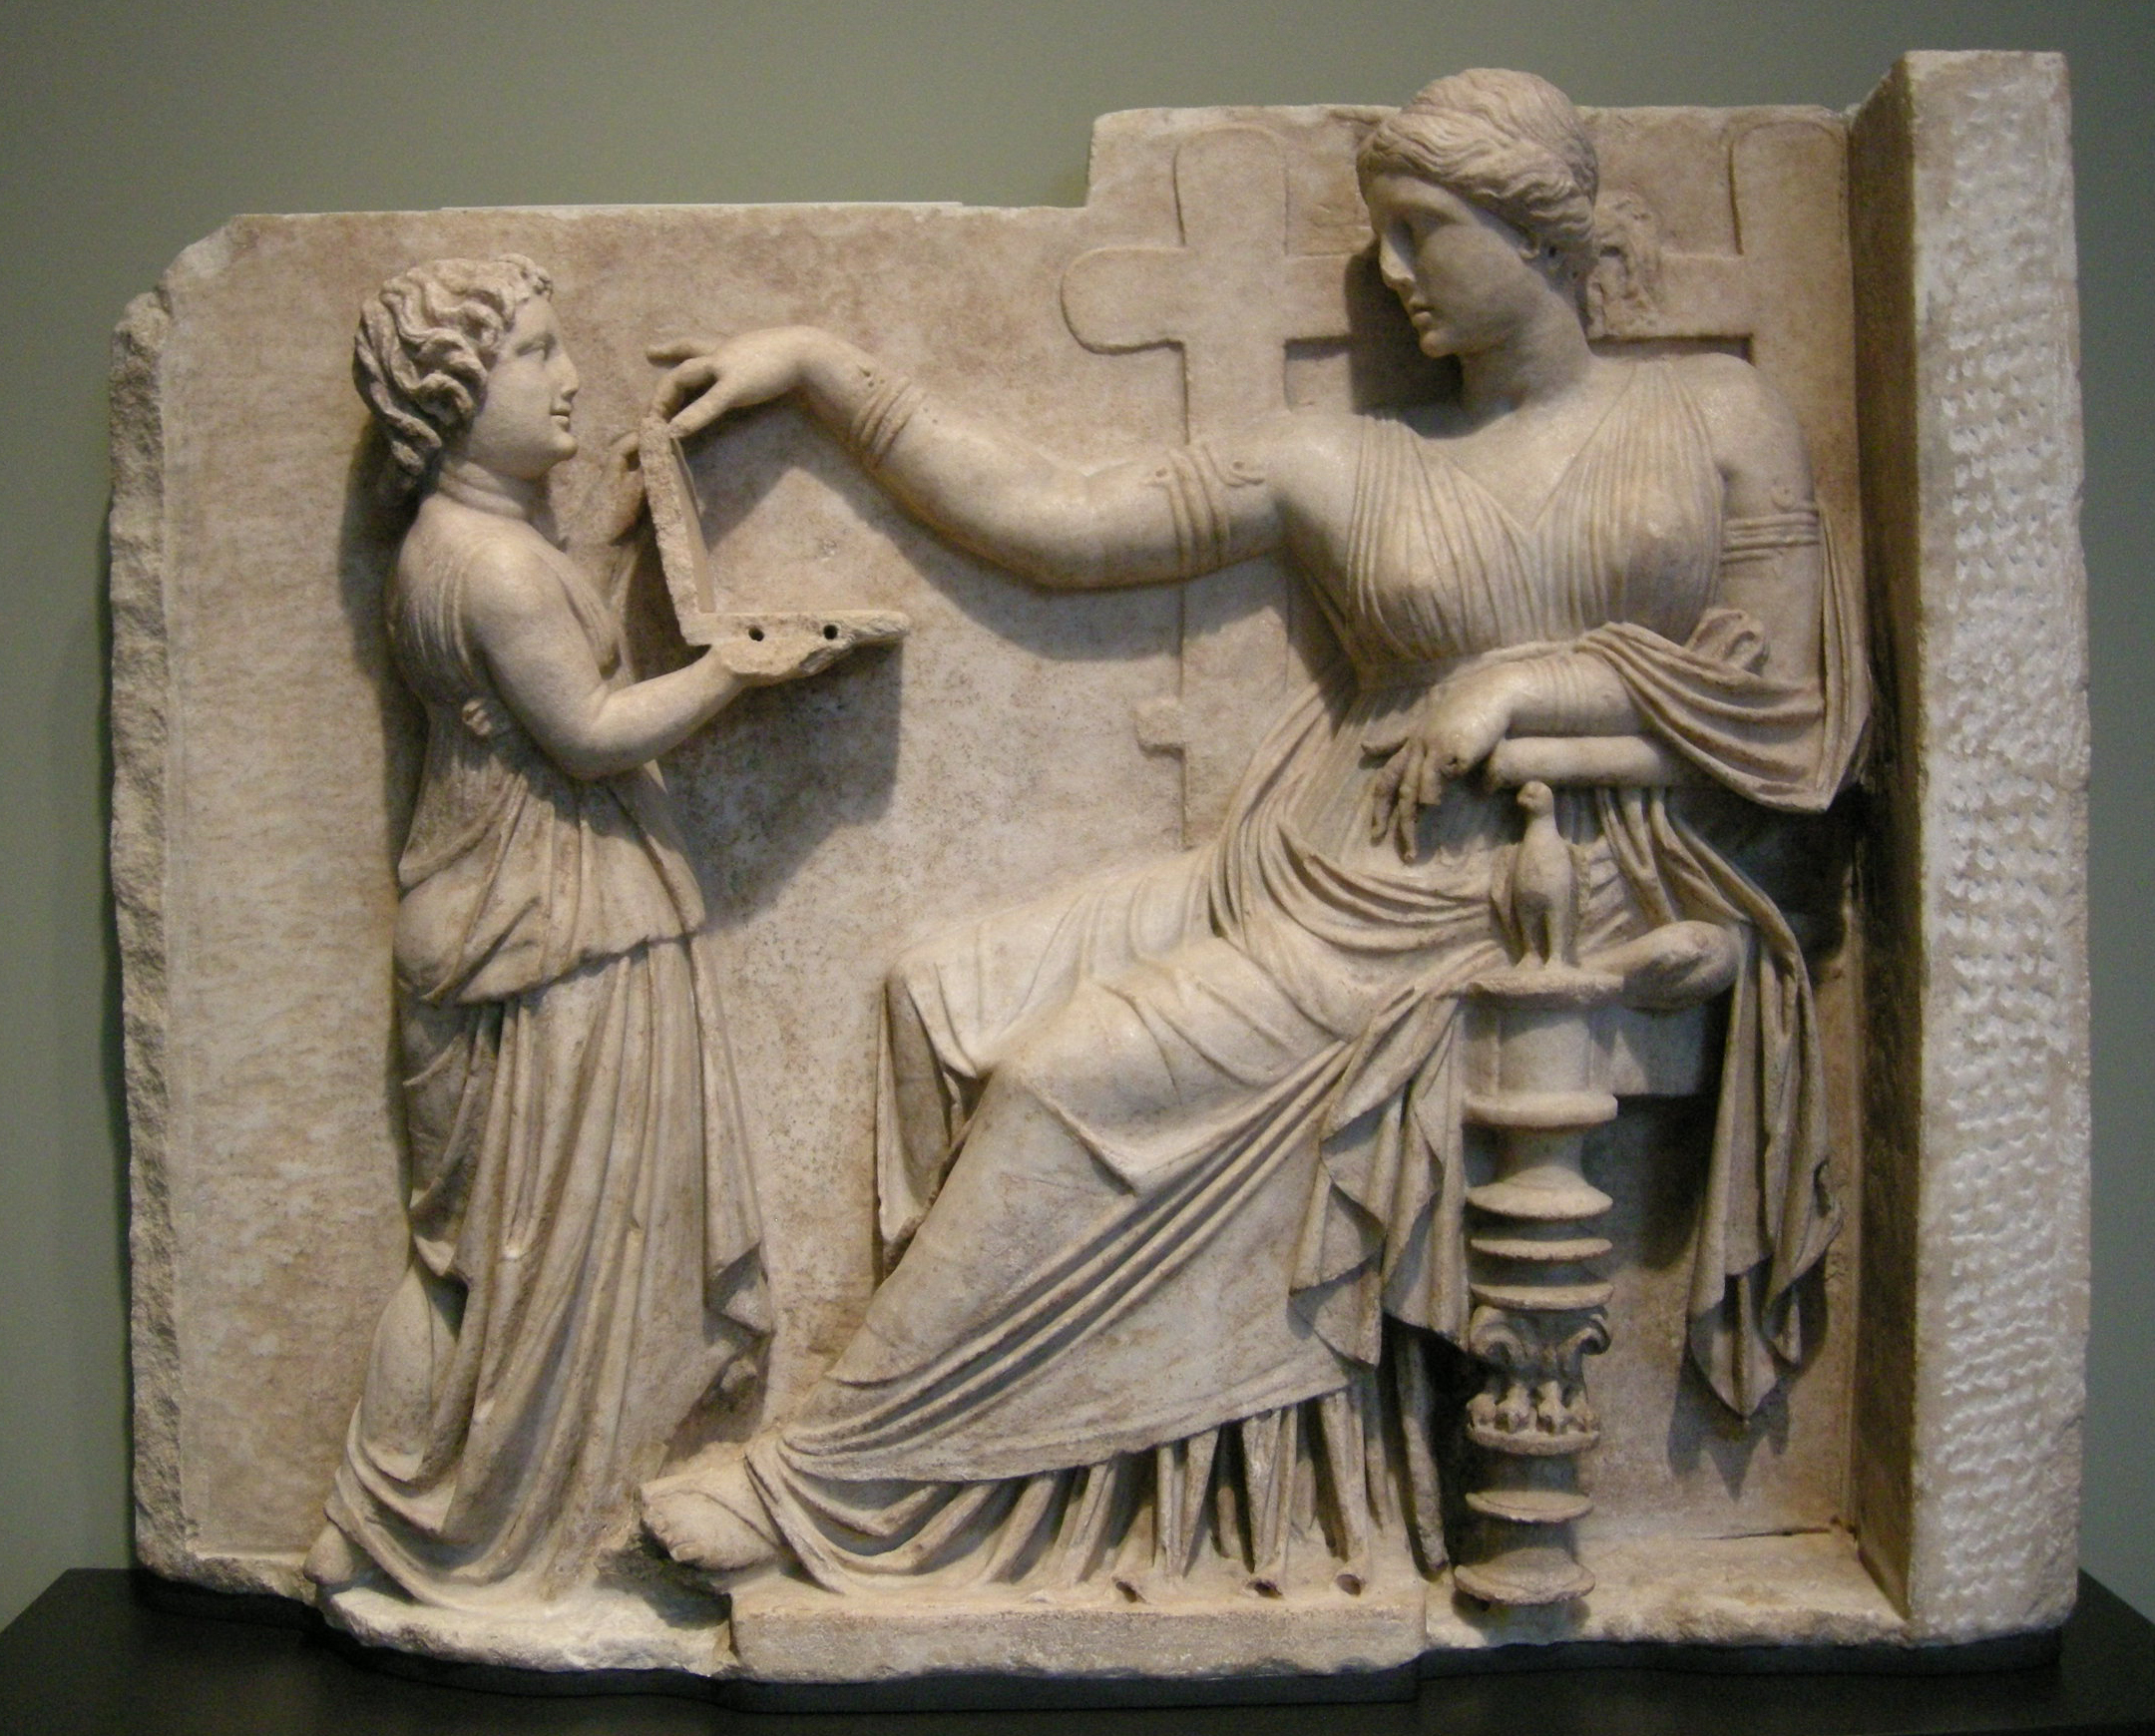
\includegraphics[height=.85\textheight]{../../../img/computador_grego.jpg}}
\usetheme{default}
\author{ \vspace{-2em} \footnotesize Pedro Bruel \newline \scriptsize \emph{phrb@ime.usp.br}}
\date{\scriptsize 6 de Agosto de 2019}
\title{ \vspace{11em} Uma Breve História  \\ da Computação}
\hypersetup{
 pdfauthor={ \vspace{-2em} \footnotesize Pedro Bruel \newline \scriptsize \emph{phrb@ime.usp.br}},
 pdftitle={ \vspace{11em} Uma Breve História  \\ da Computação},
 pdfkeywords={},
 pdfsubject={},
 pdfcreator={Emacs 26.3 (Org mode 9.2.5)},
 pdflang={Brazilian}}
\begin{document}

\maketitle

\section{Introdução}
\label{sec:orgd9eb99e}
\begin{frame}[label={sec:org13b6ea7}]{Informações Importantes}
\alert{Site} do curso:
\begin{itemize}
\item \href{https://phrb.github.io/MAC0115}{phrb.github.io/MAC0115}
\item Documento com \alert{informações importantes}: \href{https://phrb.github.io/MAC0115/pdf/MAC0115.pdf}{phrb.github.io/MAC0115/pdf/MAC0115.pdf}
\item Contém \emph{slides} e \alert{todo o material} de apoio às aulas
\end{itemize}
\emph{Moodle} do curso no \alert{\emph{PACA}}:
\begin{itemize}
\item \href{https://paca.ime.usp.br/course/view.php?id=1448}{paca.ime.usp.br/course/view.php?id=1448}
\item O PACA é o site dos cursos do IME/USP. \alert{Faça sua conta} para acessar!
\end{itemize}
\alert{Livro} usado no curso:
\begin{itemize}
\item \href{https://phrb.github.io/PenseJulia}{phrb.github.io/PenseJulia}
\item Usa \alert{\emph{Notebooks Jupyter}}
\end{itemize}
\end{frame}

\begin{frame}[label={sec:org962b105}]{Licença}
Esta aula é disponibilizada sob \alert{licença Creative Commons}:
\begin{figure}[htbp]
\centering

\includegraphics[width=0.3\textwidth]{../../../img/by-nc.png}
\caption{\href{https://creativecommons.org/licenses/by-nc/3.0/deed.pt}{Atribuição-NãoComercial 3.0 Não Adaptada (CC BY-NC 3.0)}}
\end{figure}

A maioria das imagens vem do \alert{Wikimedia Commons}:
\begin{figure}[htbp]
\centering

\includegraphics[width=0.1\textwidth]{../../../img/wikimedia_commons.jpg}
\caption{\href{https://commons.wikimedia.org/wiki/Main_Page}{Wikimedia Commons}}
\end{figure}
\end{frame}
\begin{frame}[label={sec:org85def95}]{Uma Breve História da Computação}
\begin{figure}[htbp]
\centering
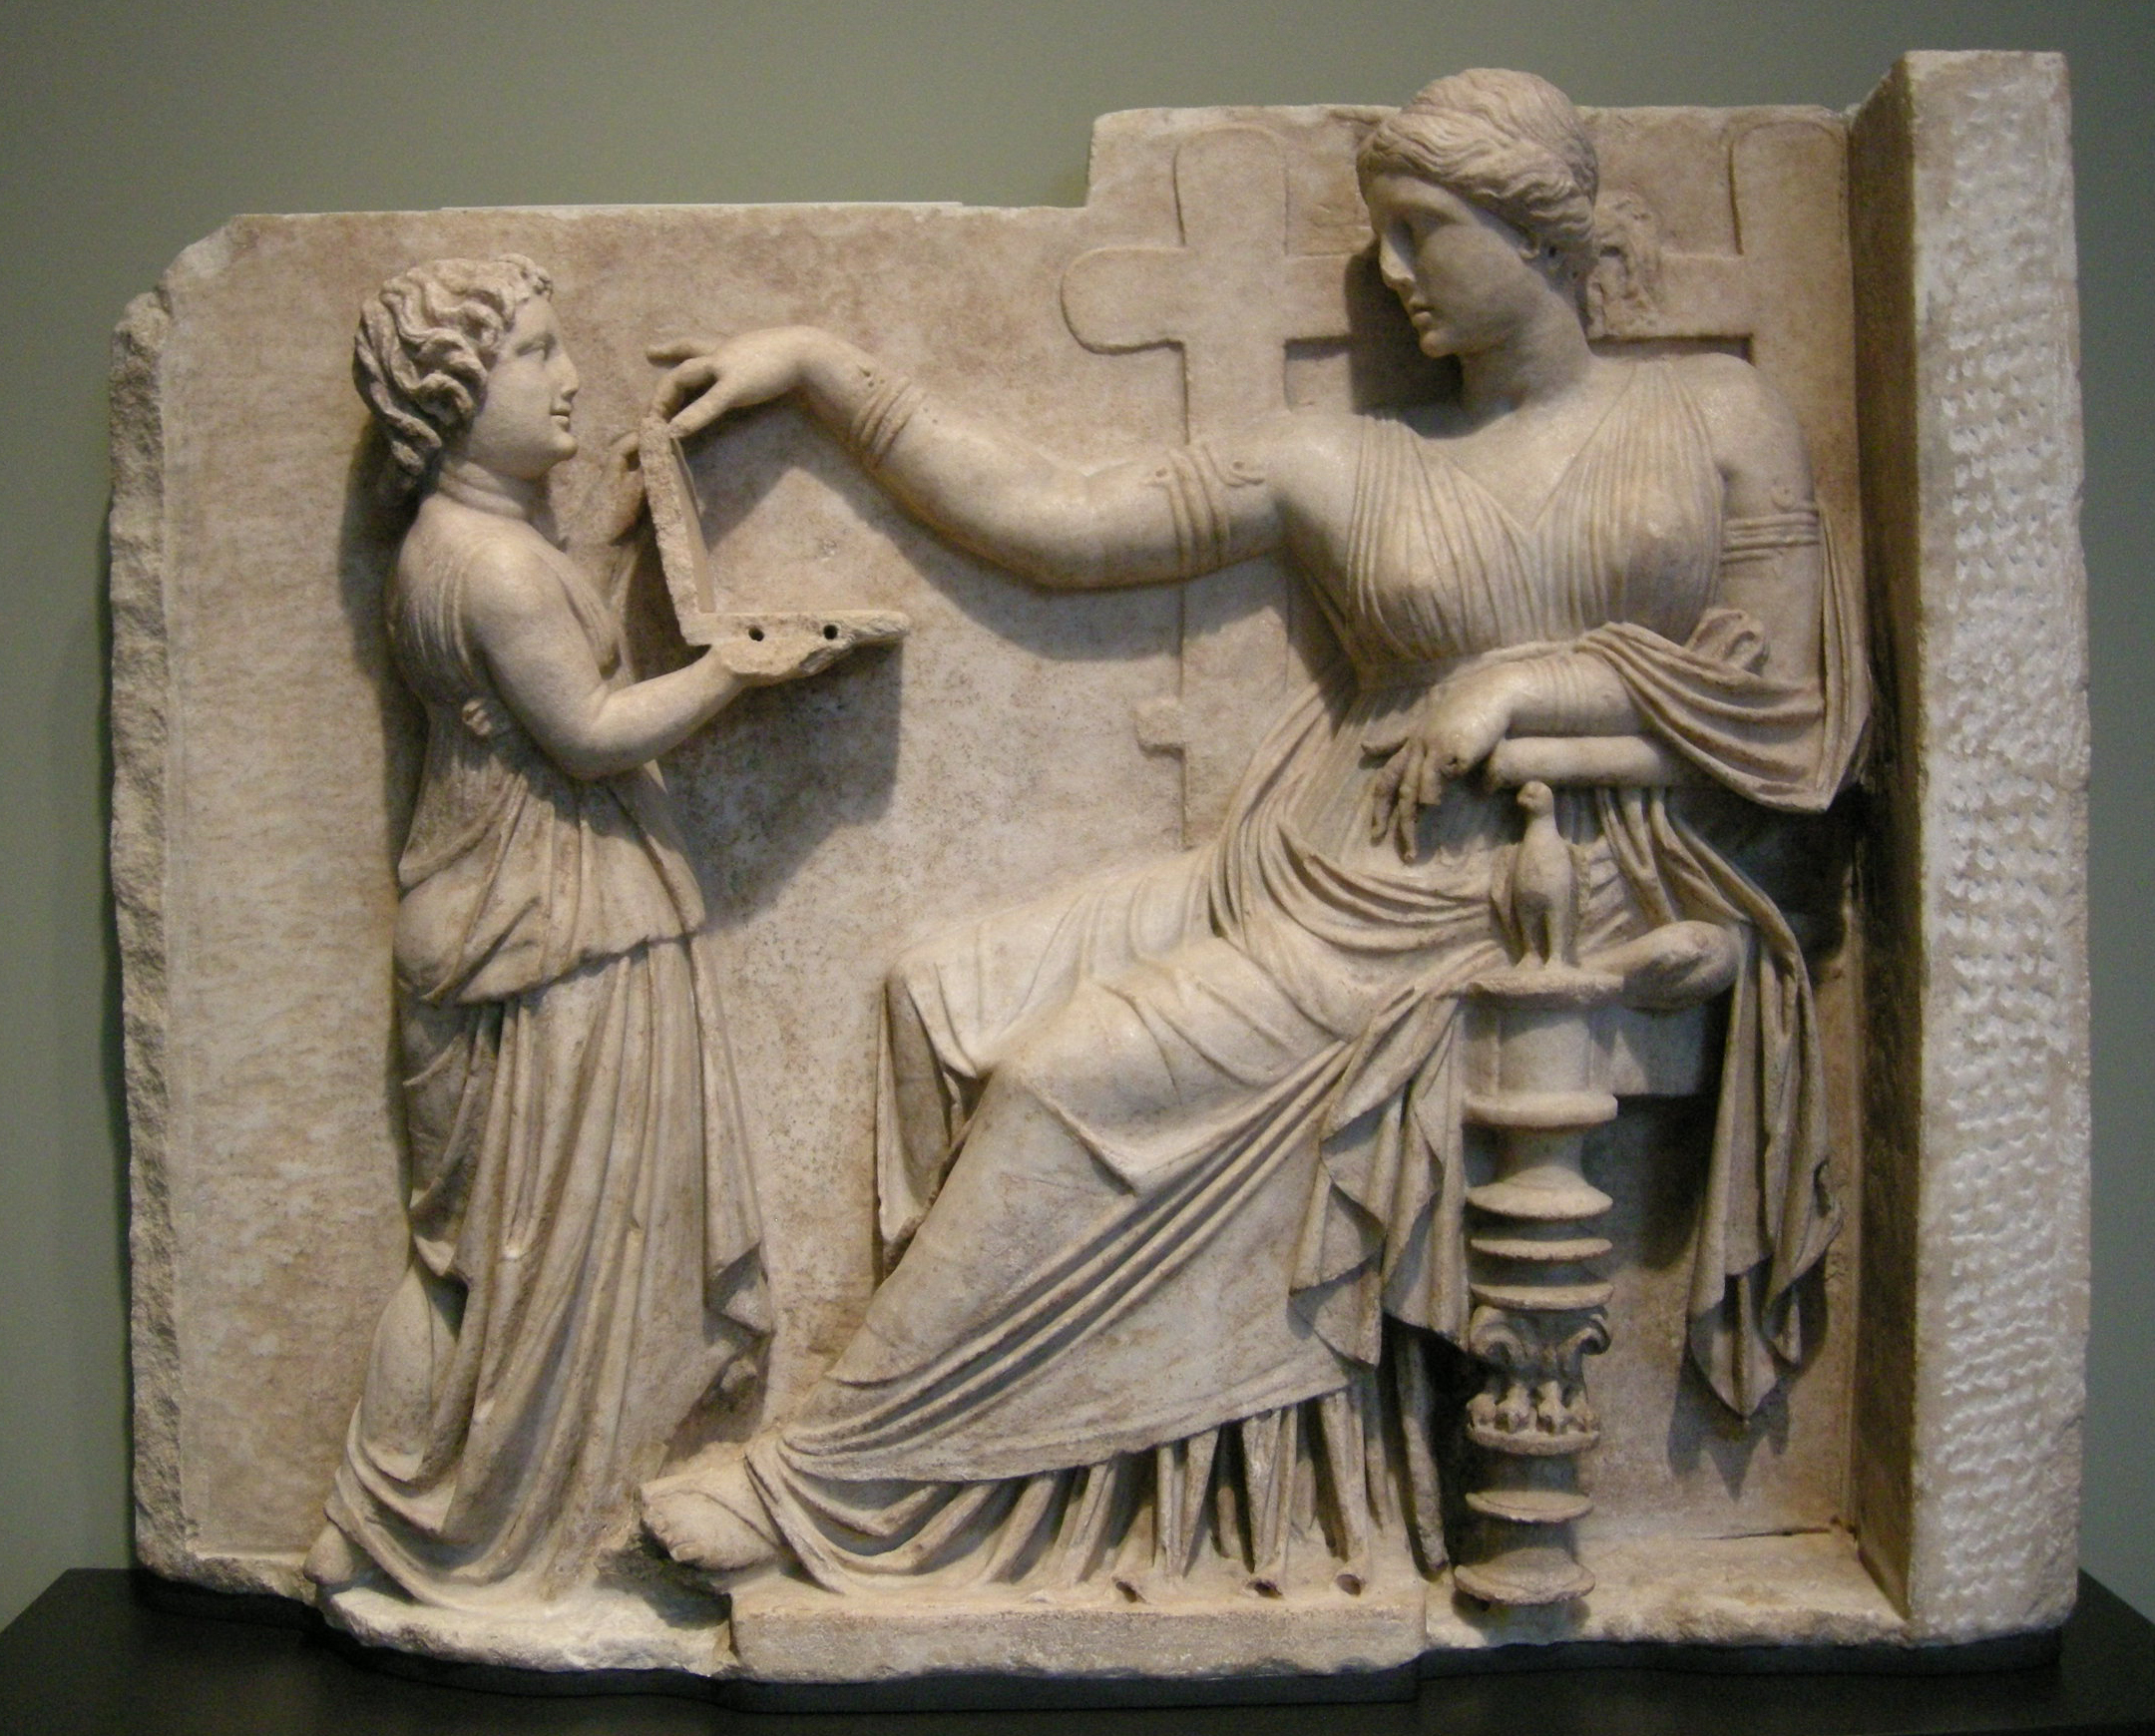
\includegraphics[height=.8\textheight]{../../../img/computador_grego.jpg}
\caption{Pedra tumular, Grécia, \textasciitilde{100 AC} (Getty Villa, \alert{não é um notebook})}
\end{figure}
\end{frame}
\begin{frame}[label={sec:orgadf1db2}]{Uma Breve História da Computação: Sobre Esta Aula}
\begin{columns}
\begin{column}{0.5\columnwidth}
\begin{block}{Computação}
\begin{itemize}
\item \alert{O que é}?
\item \alert{Desde quando} existe?
\item Qual é sua \alert{utilidade}?
\end{itemize}

\begin{block}{Roteiro desta Aula}
\begin{enumerate}
\item Computação até o \alert{Século 19}
\item Computação \alert{Moderna}
\item Computação e \alert{Ciência}
\end{enumerate}
\end{block}
\end{block}
\end{column}

\begin{column}{0.5\columnwidth}
\begin{block}{O que pode ser Computação?}
\only<1>{
\begin{figure}[htbp]
\centering
\includegraphics[width=\columnwidth]{../../../img/summit_supercomputer.jpg}
\caption{\alert{Supercomputador} Summit}
\end{figure}
}

\only<2>{
\begin{figure}[htbp]
\centering
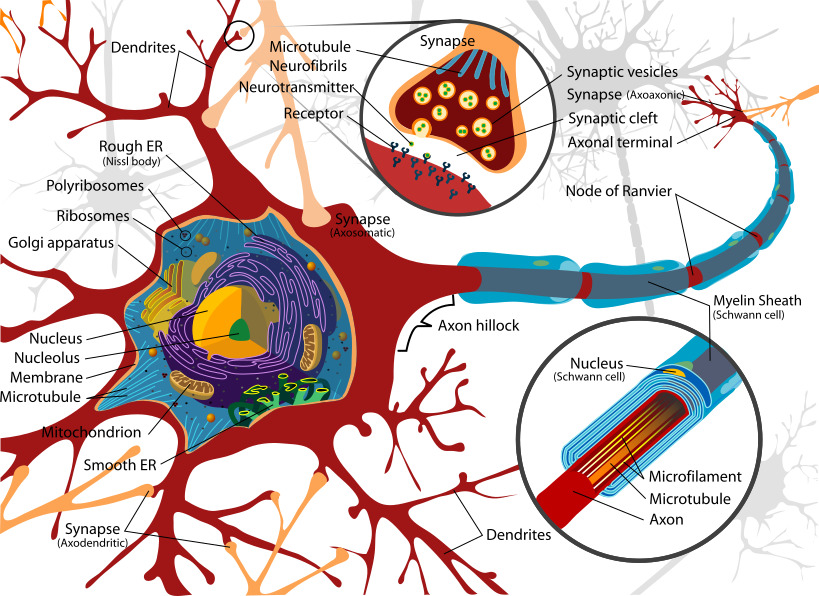
\includegraphics[width=.8\columnwidth]{../../../img/neuron.jpg}
\caption{\alert{Neurônio}}
\end{figure}
}

\only<3>{
\begin{figure}[htbp]
\centering
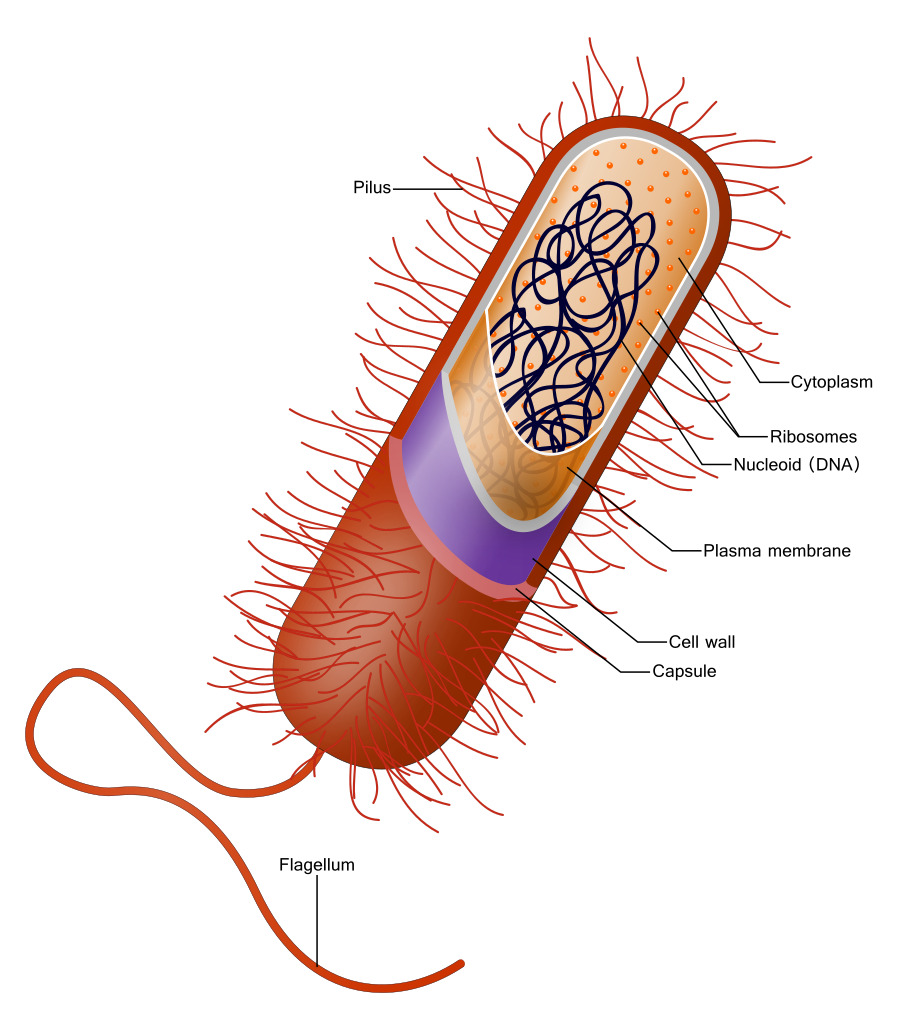
\includegraphics[width=.55\columnwidth]{../../../img/procaryote.jpg}
\caption{Célula \alert{procarionte}}
\end{figure}
}

\only<4>{
\begin{figure}[htbp]
\centering
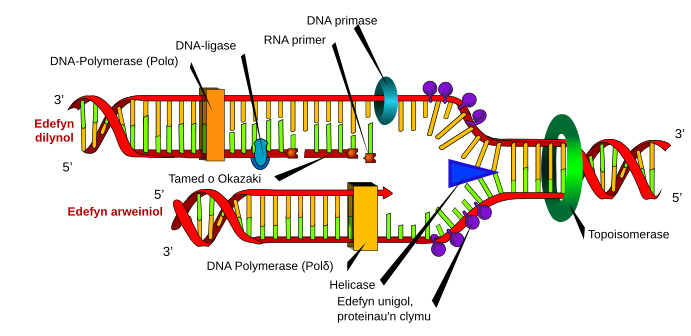
\includegraphics[width=.8\columnwidth]{../../../img/dna.jpg}
\caption{Processo (\alert{algoritmo}?) de \alert{duplicação do DNA}}
\end{figure}
}

\only<5>{
\begin{figure}[htbp]
\centering
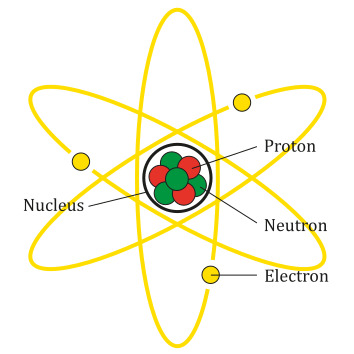
\includegraphics[width=.65\columnwidth]{../../../img/atom.jpg}
\caption{Representação de um \alert{átomo}}
\end{figure}
}
\end{block}
\end{column}
\end{columns}
\end{frame}

\begin{frame}[label={sec:orga0d3e1d}]{Tecnologia Computacional na Antiguidade: Melhores Usos\dots{}}
\begin{figure}[htbp]
\centering
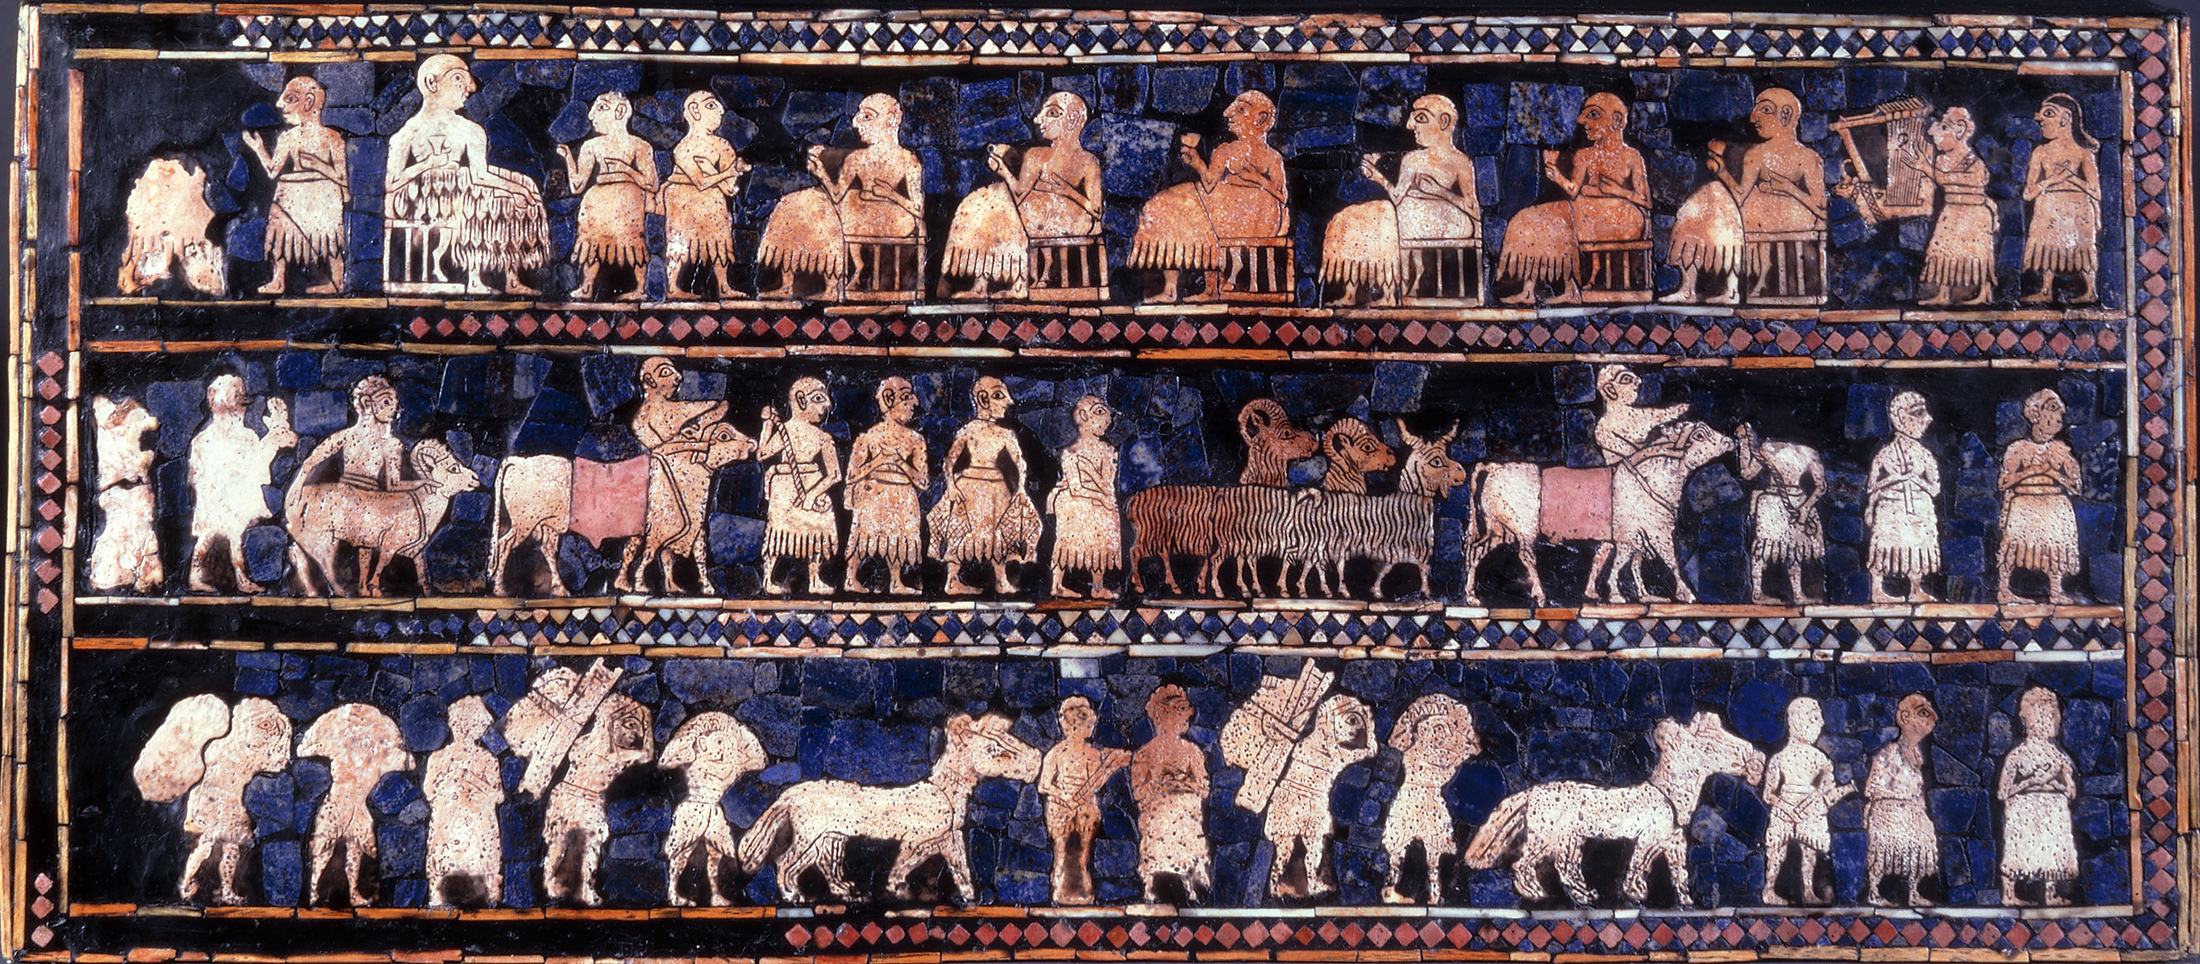
\includegraphics[width=\textwidth]{../../../img/ur_estandarte_paz.jpg}
\caption{Estandarte de Ur, \alert{lado paz}, 2600 AC}
\end{figure}
\end{frame}
\begin{frame}[label={sec:org972c679}]{Tecnologia Computacional na Antiguidade: \dots{}Piores Usos}
\begin{figure}[htbp]
\centering
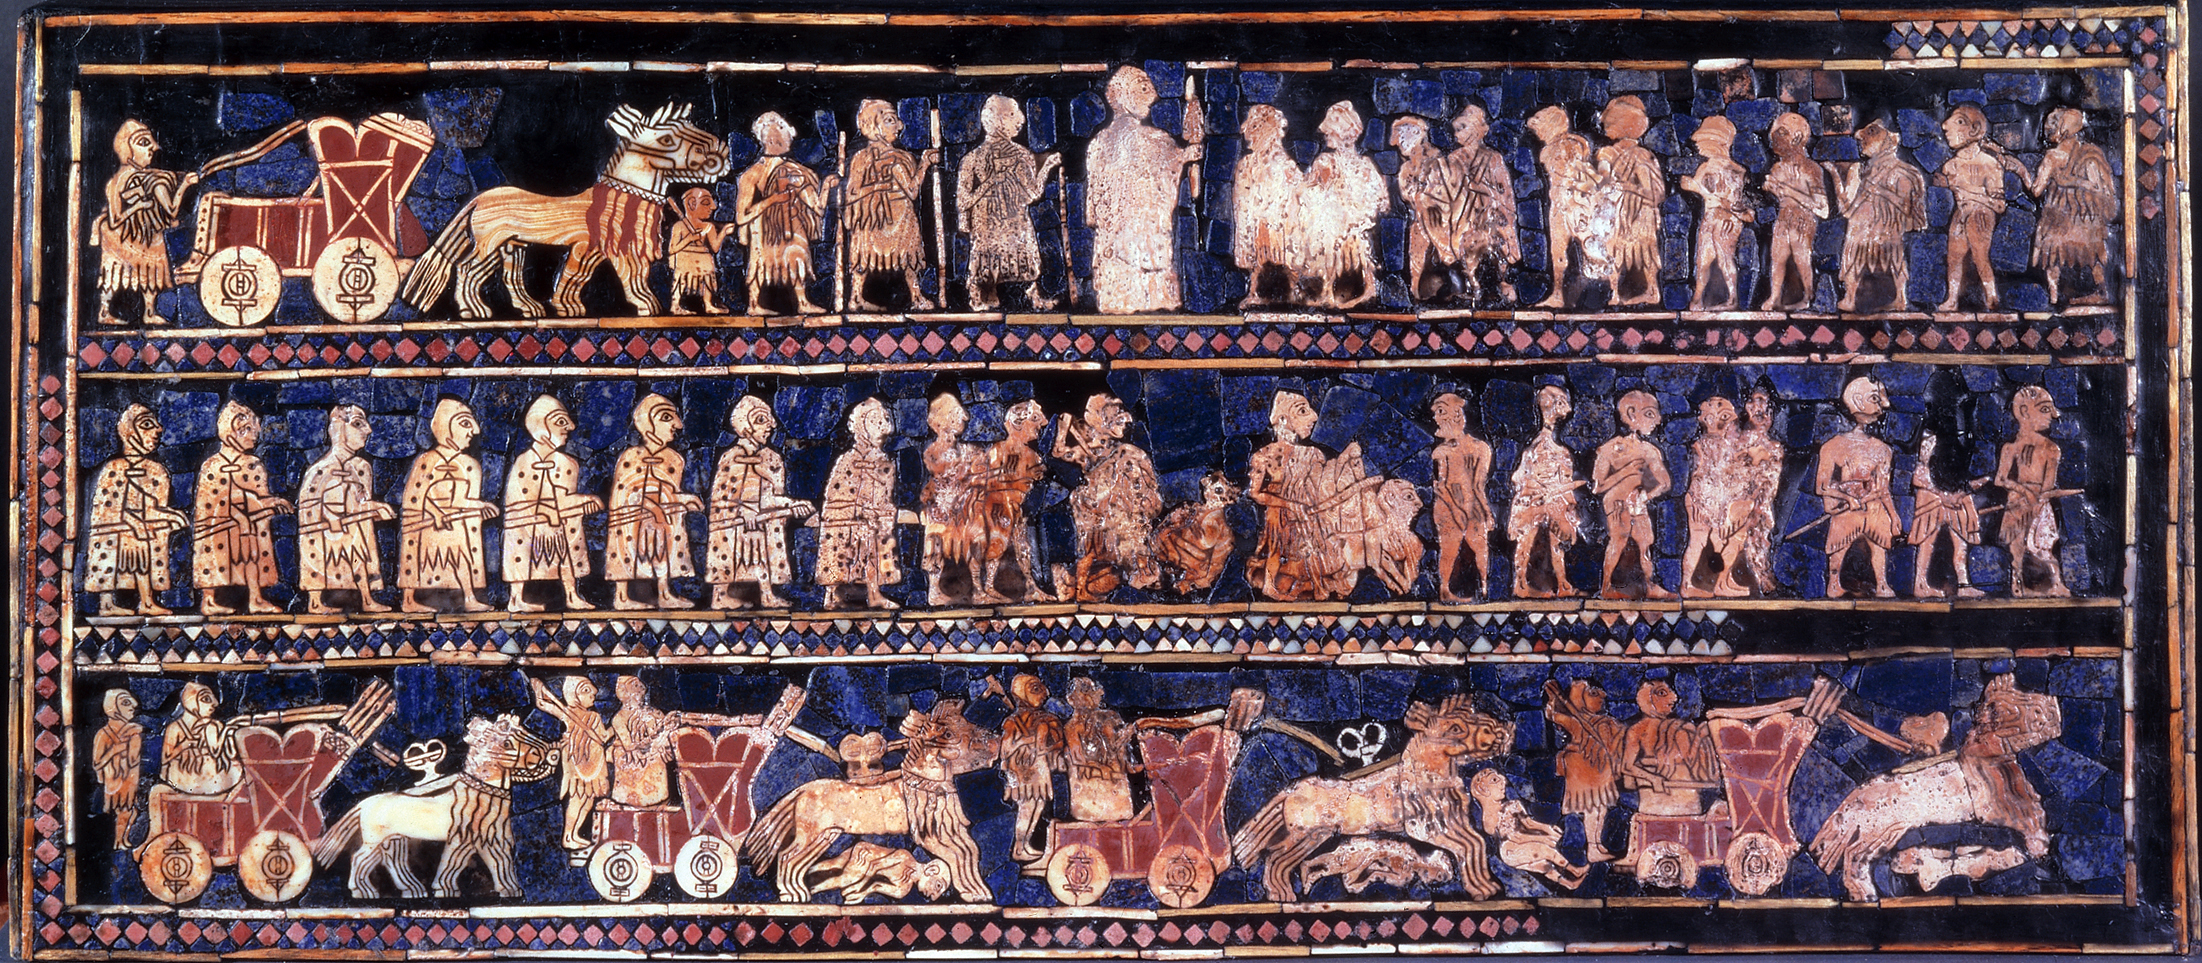
\includegraphics[width=\textwidth]{../../../img/ur_estandarte_guerra.jpg}
\caption{Estandarte de Ur, \alert{lado guerra}, 2600 AC}
\end{figure}
\end{frame}
\section{Primórdios da Computação}
\label{sec:org315fd75}
\begin{frame}[label={sec:org9174d7f}]{Primórdios da Computação: O Ábaco}
\begin{columns}
\begin{column}{0.5\columnwidth}
\begin{block}{História do \alert{Ábaco}}
\begin{itemize}
\item Egípcios, \alert{Sumérios}: \textasciitilde{}3000 AC
\item Persas: \textasciitilde{}600 AC
\item \visible<2->{Gregos: \textasciitilde{}384 AC}
\item \visible<3->{Chineses: \textasciitilde{}200 AC}
\item \visible<7->{Romanos: \textasciitilde{}100 AC}
\item \visible<8->{\alert{Indianos e Árabes}: \textasciitilde{}100}
\item \visible<9->{Américas: \textasciitilde{}1300}
\end{itemize}
\end{block}
\end{column}

\begin{column}{0.5\columnwidth}
\only<1>{
\begin{figure}[htbp]
\centering
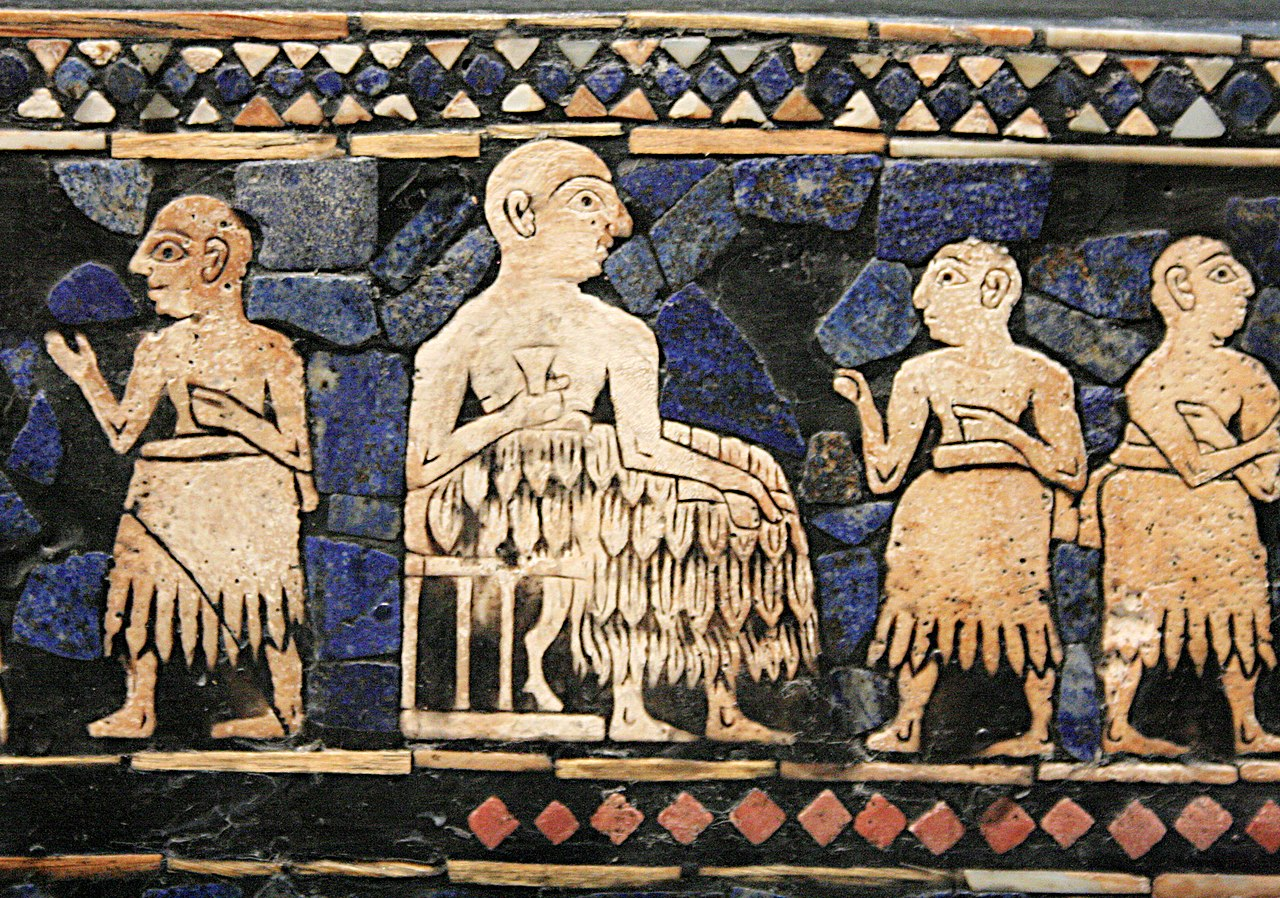
\includegraphics[width=\columnwidth]{../../../img/rei_de_ur_2600BC.jpg}
\caption{Rei de Ur, Mesopotâmia, 2600 AC}
\end{figure}
}

\only<2>{
\begin{figure}[htbp]
\centering
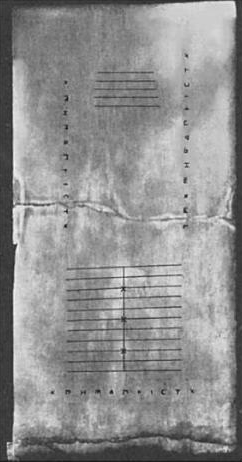
\includegraphics[width=.4\columnwidth]{../../../img/tablete_salamis_gregos.jpg}
\caption{\alert{Tábua de Contagem} Salamina, 300 AC}
\end{figure}
}

\only<3>{
\begin{figure}[htbp]
\centering
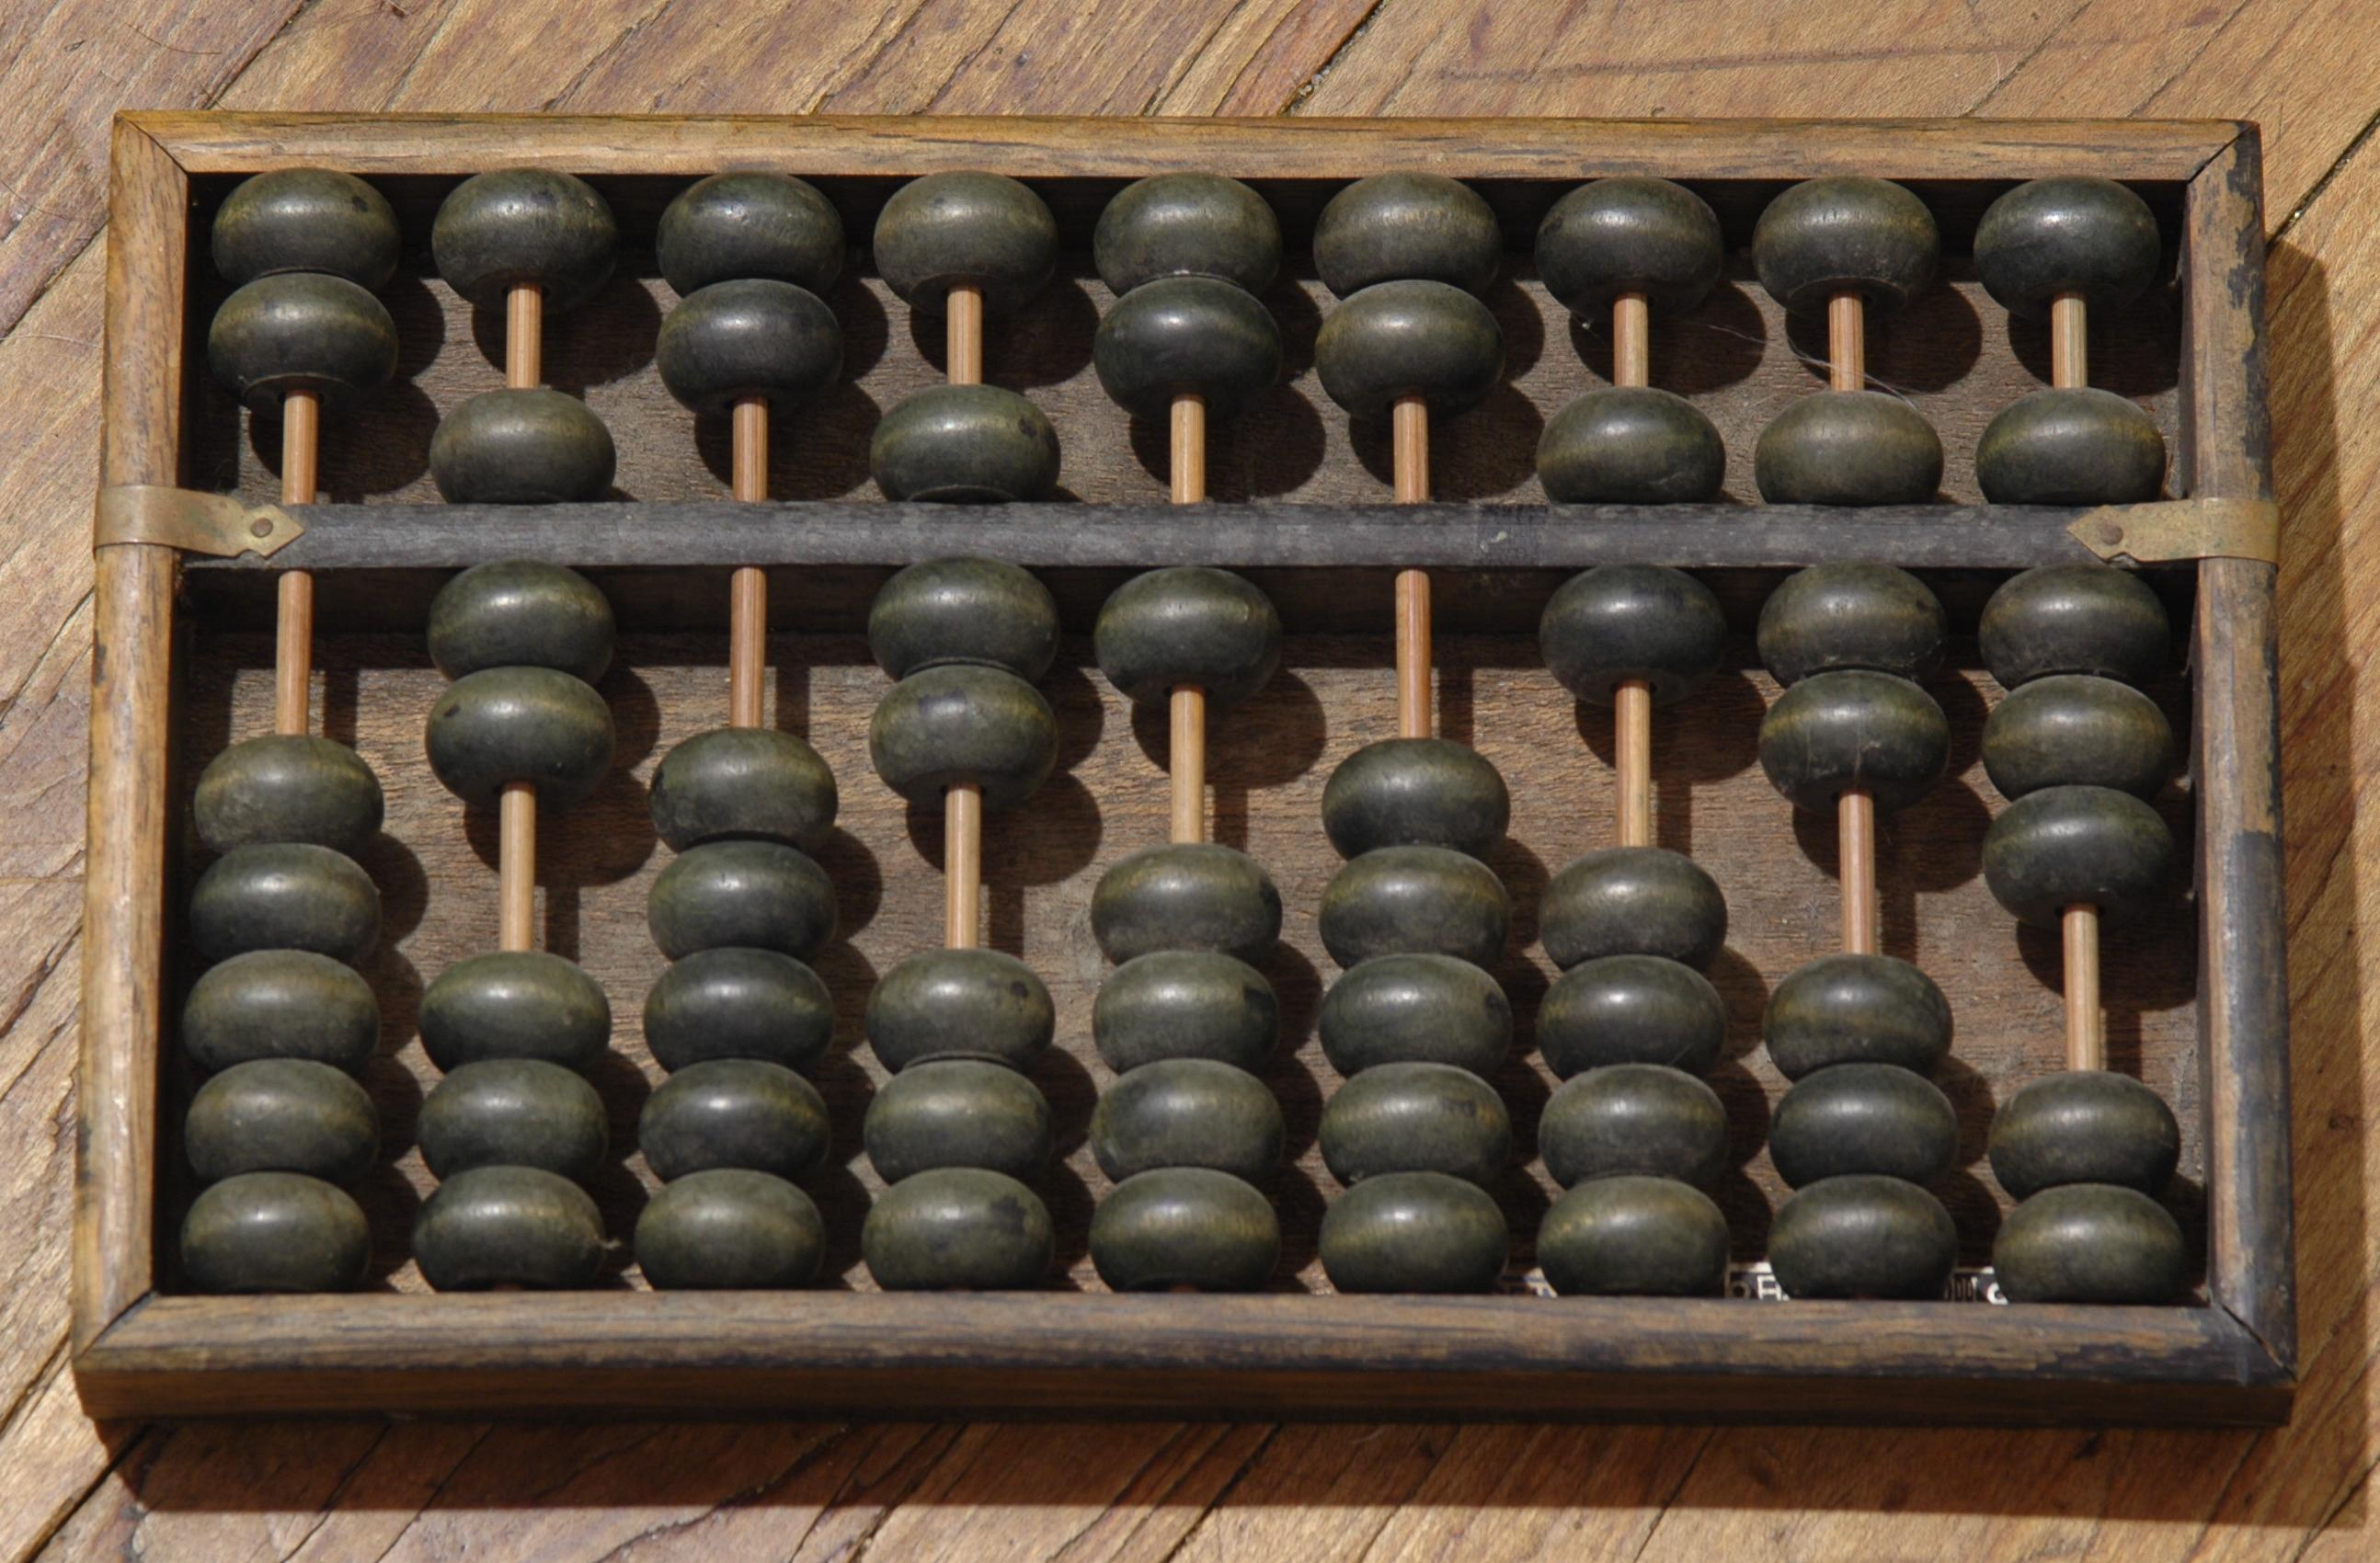
\includegraphics[width=\columnwidth]{../../../img/abaco_chines.jpg}
\caption{\alert{算盤} (\alert{Suanpan}), Ábaco Chinês}
\end{figure}
}

\only<4>{
\begin{figure}[htbp]
\centering
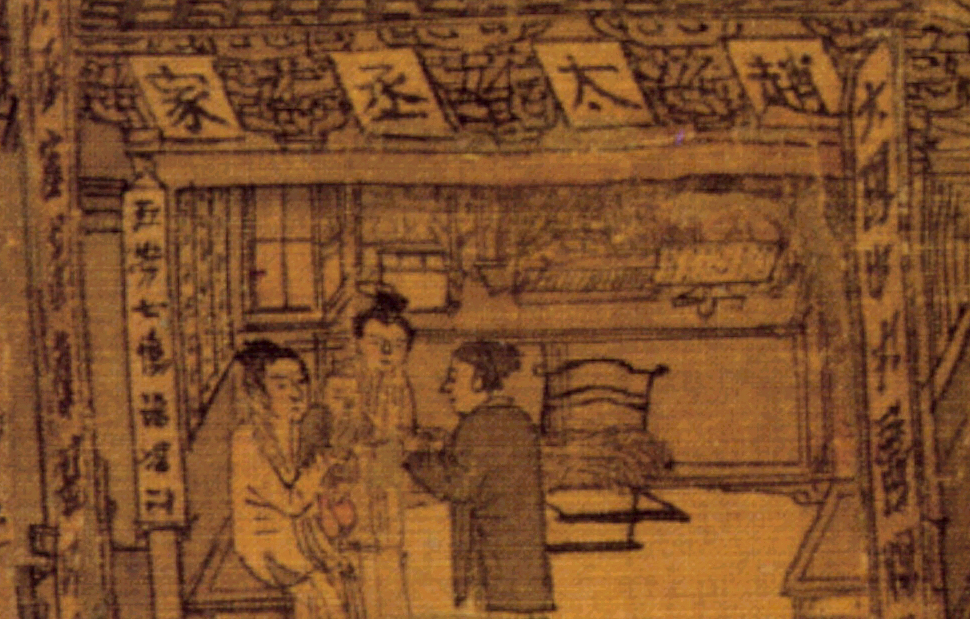
\includegraphics[width=\columnwidth]{../../../img/abaco_chines_2.jpg}
\caption{Apotecário, \textasciitilde{} 1085. Você consegue \alert{achar o ábaco}?}
\end{figure}
}

\only<5>{
\begin{figure}[htbp]
\centering
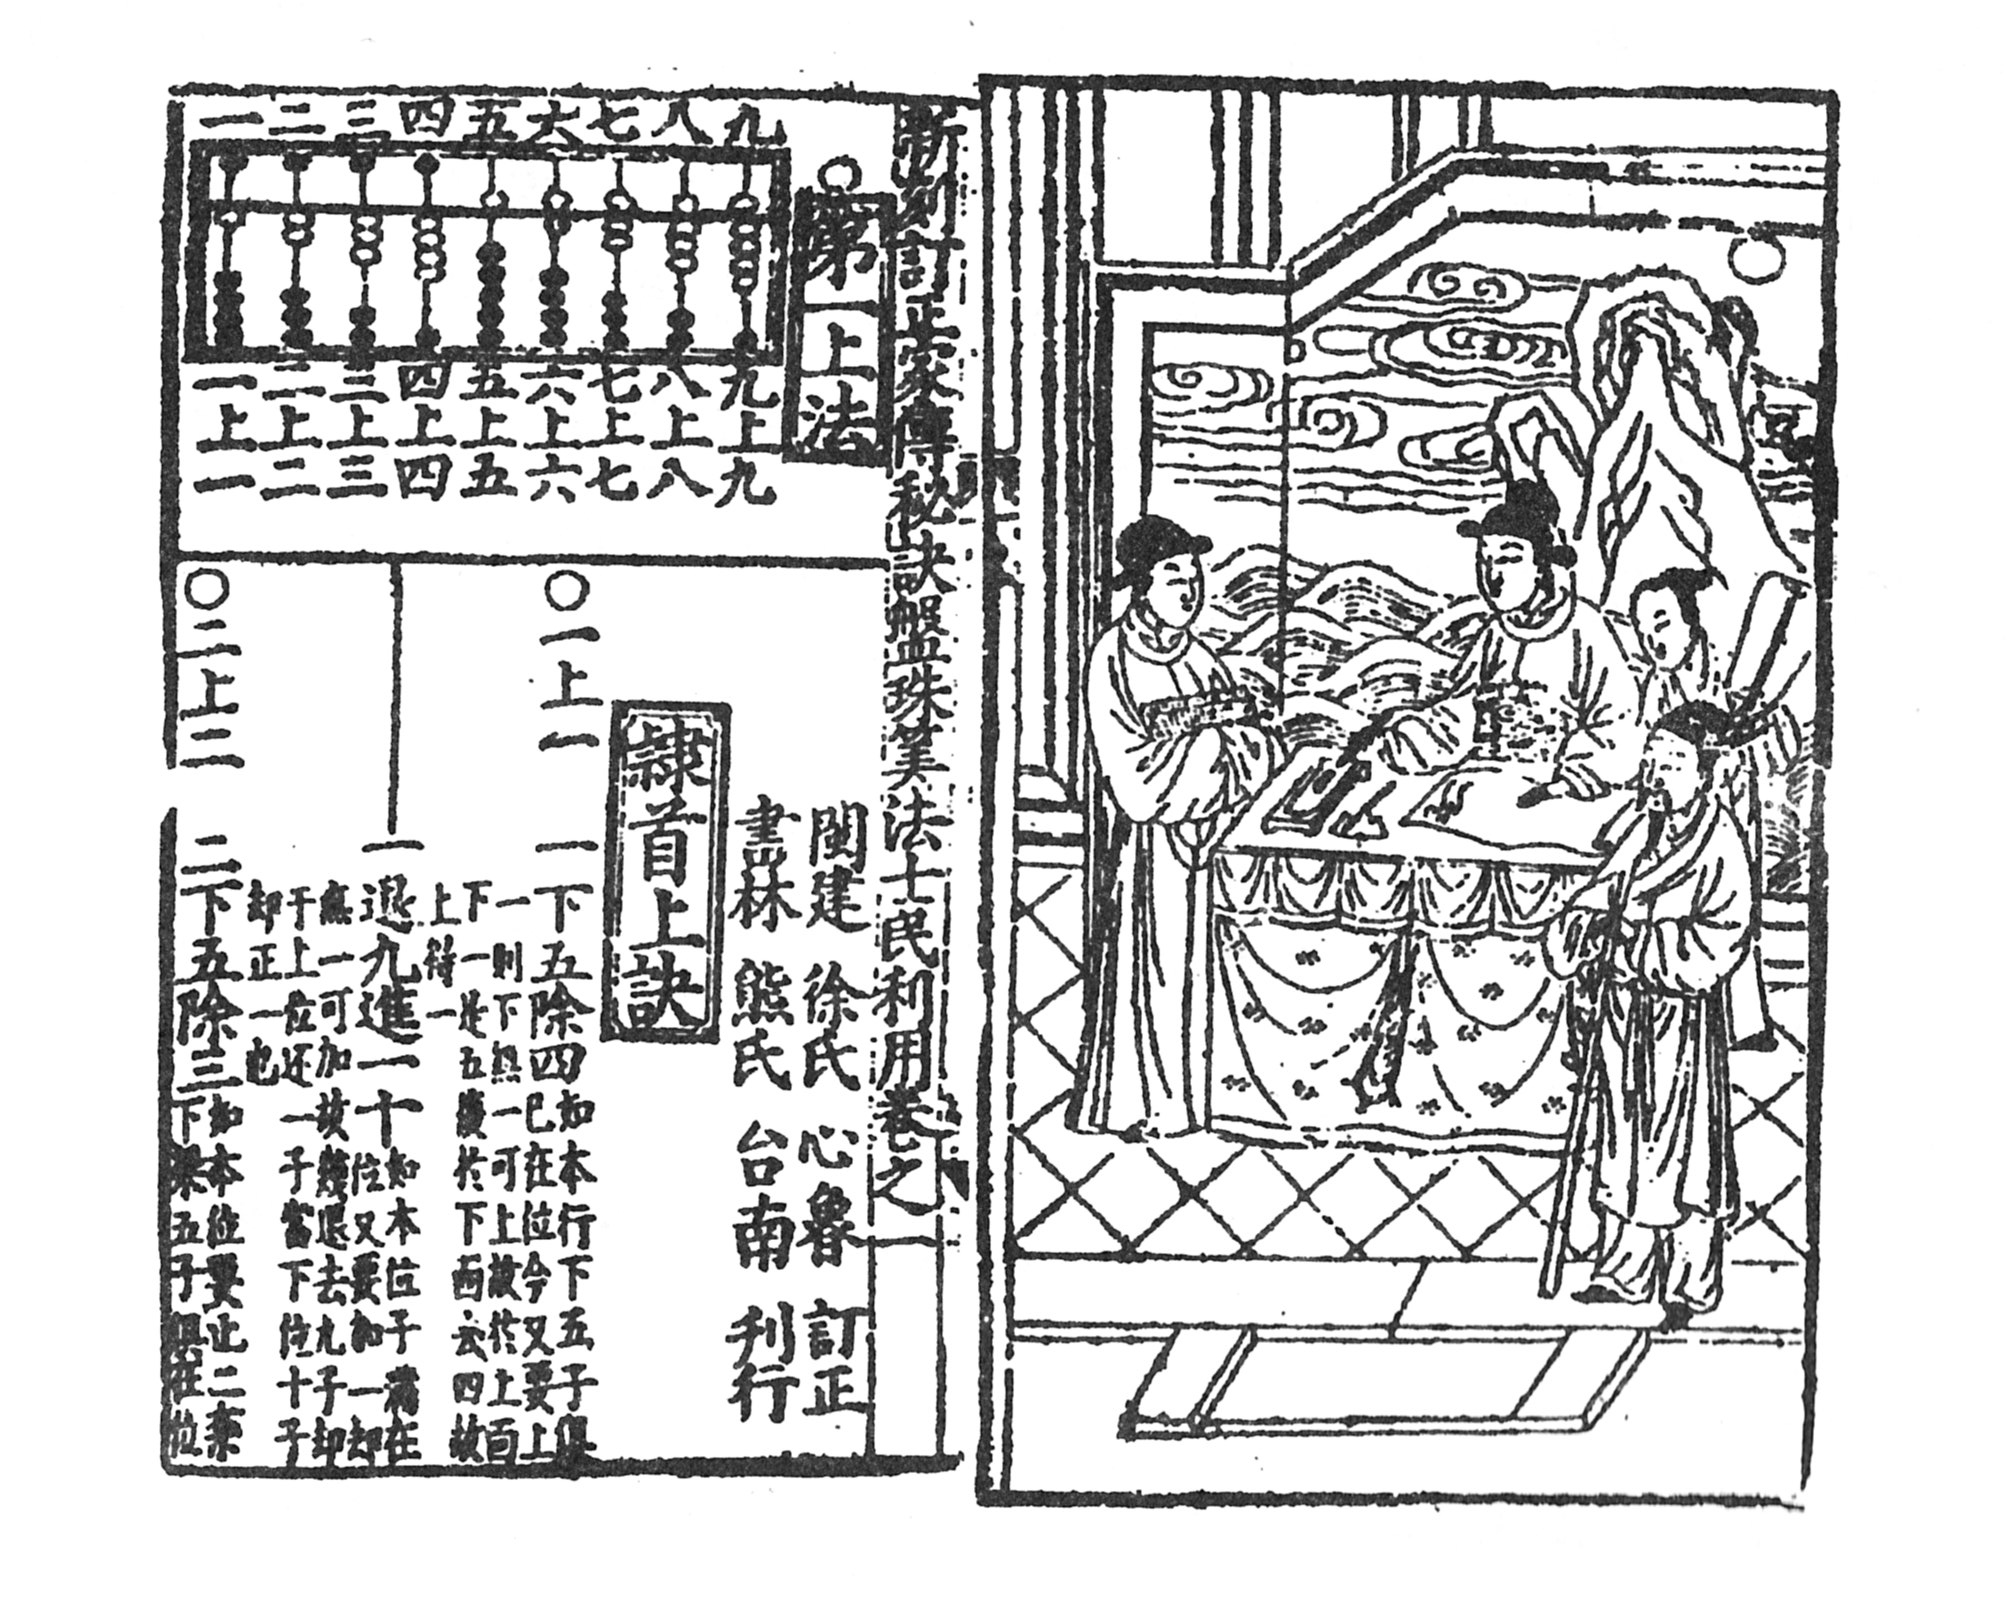
\includegraphics[width=\columnwidth]{../../../img/abaco_chines_3.jpg}
\caption{\alert{盘珠算法} (Introdução ao Ábaco), 1573}
\end{figure}
}

\only<6>{
\begin{figure}[htbp]
\centering
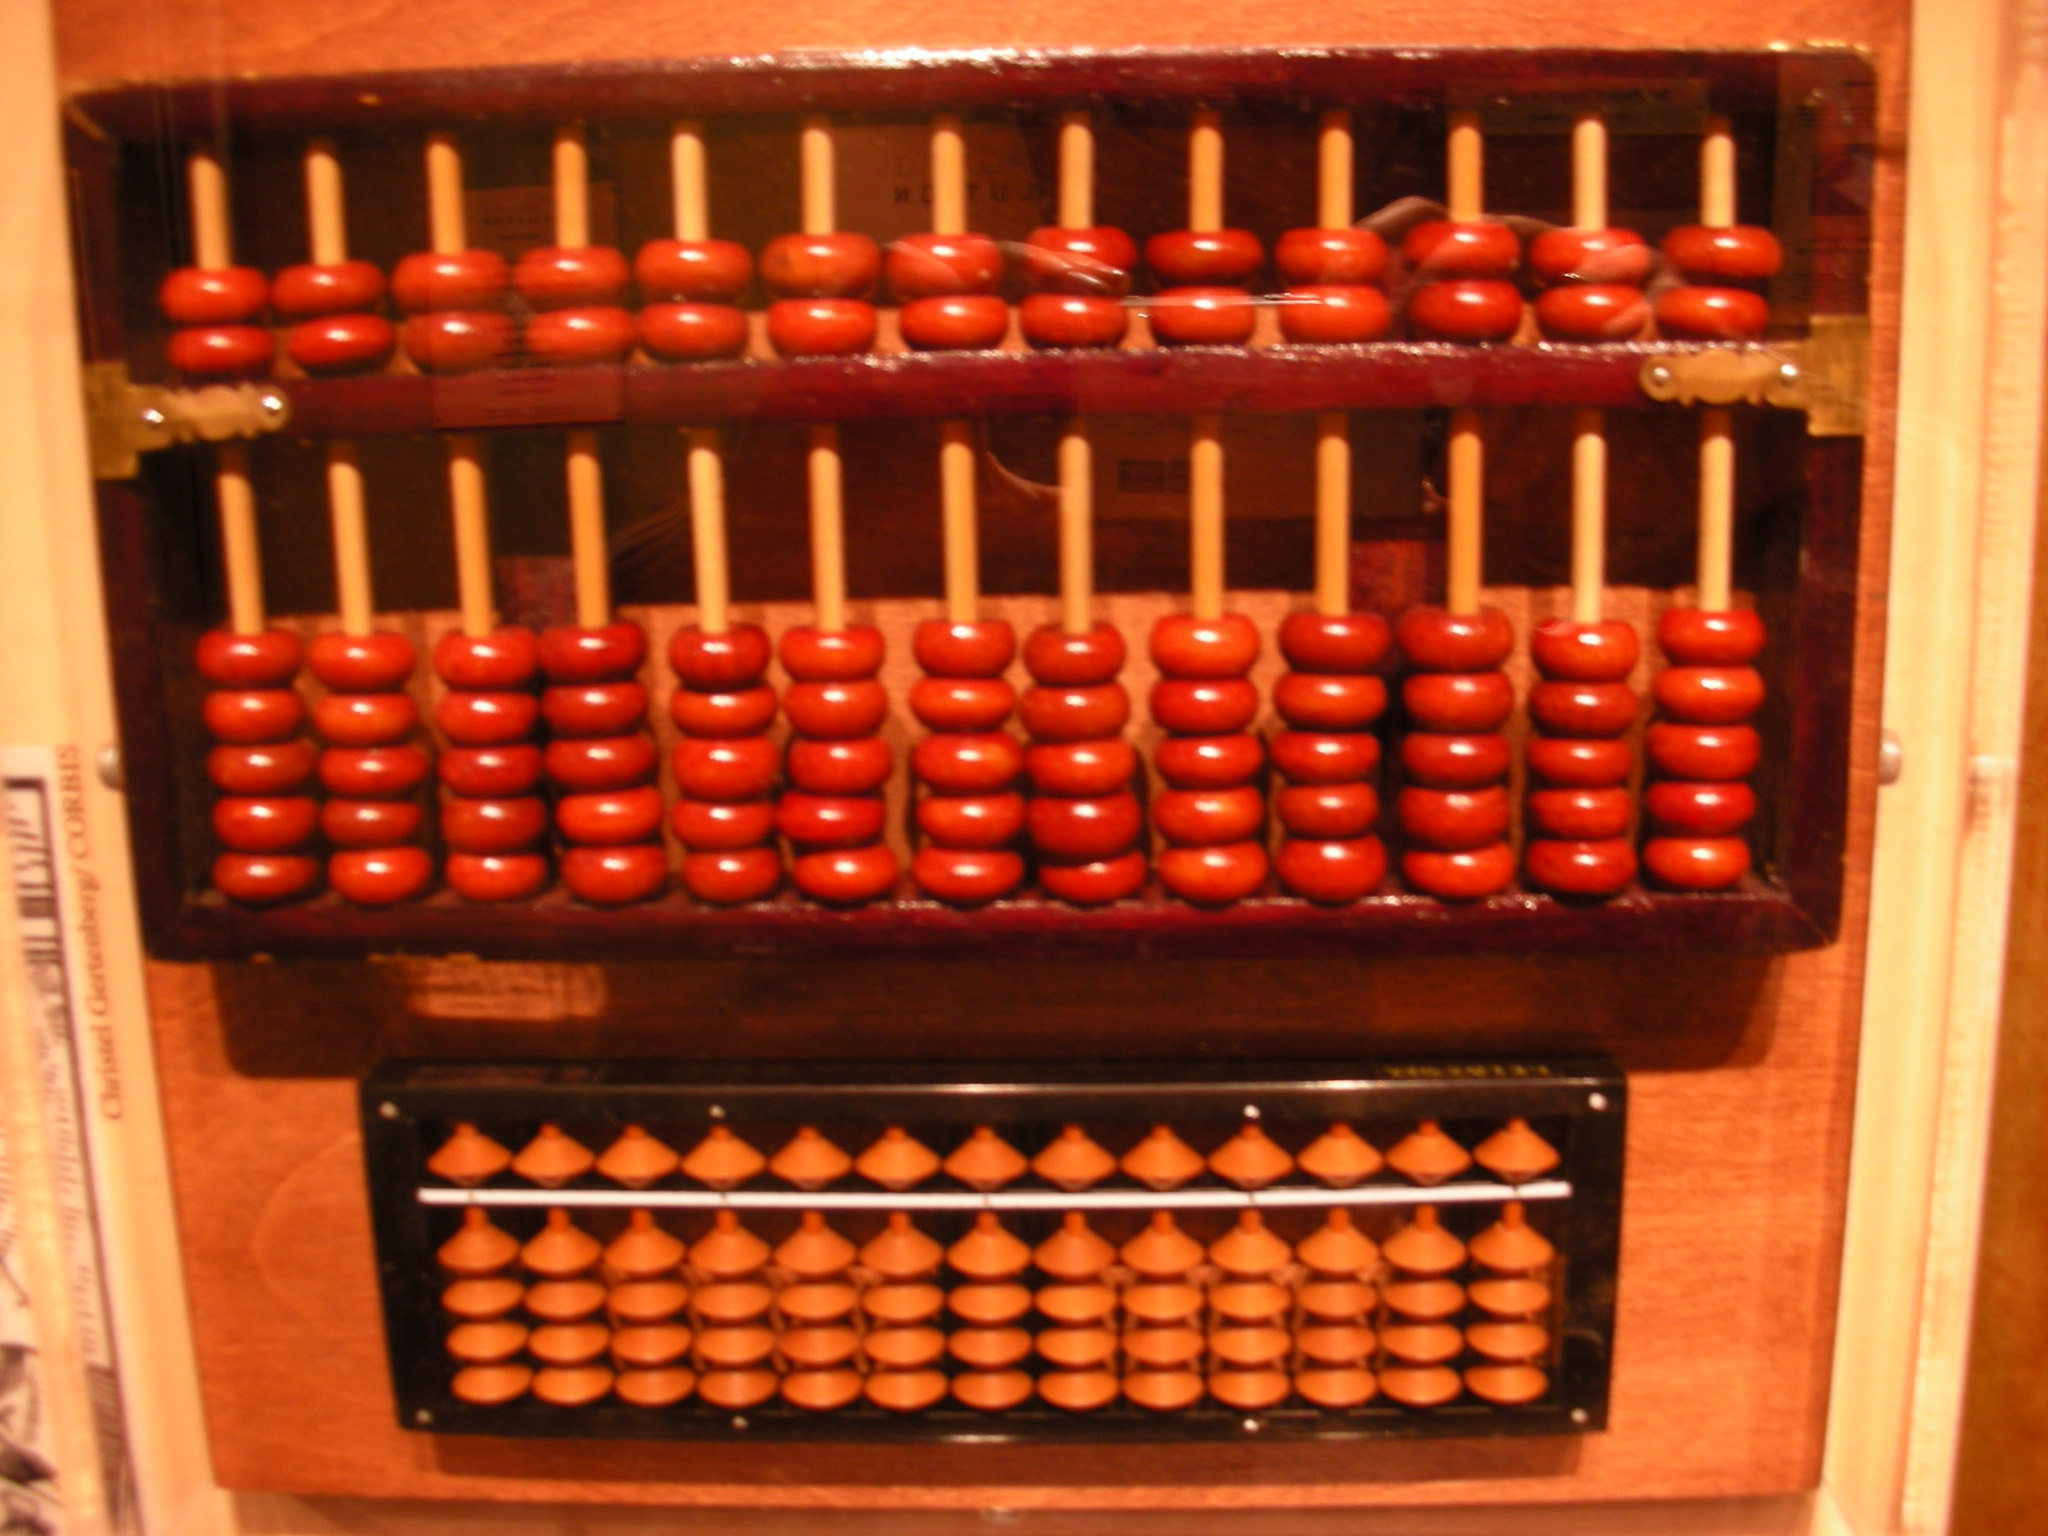
\includegraphics[width=\columnwidth]{../../../img/suanpan_soroban.jpg}
\caption{\alert{算盤}, \alert{そろばん} (\alert{Suanpan} e \alert{Soroban})}
\end{figure}
}

\only<7>{
\begin{figure}[htbp]
\centering
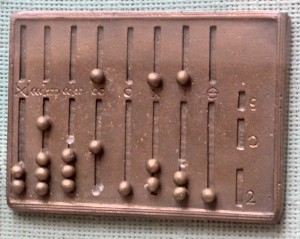
\includegraphics[width=\columnwidth]{../../../img/abaco_romano.jpg}
\caption{Reprodução de um \alert{ábaco Romano}}
\end{figure}
}

\only<8>{
\begin{figure}[htbp]
\centering
\includegraphics[width=.93\columnwidth]{../../../img/algarismos.png}
\caption{Evolução do \alert{Sistema Numérico Hindu-Arábico}}
\end{figure}
}

\only<9>{
\begin{figure}[htbp]
\centering
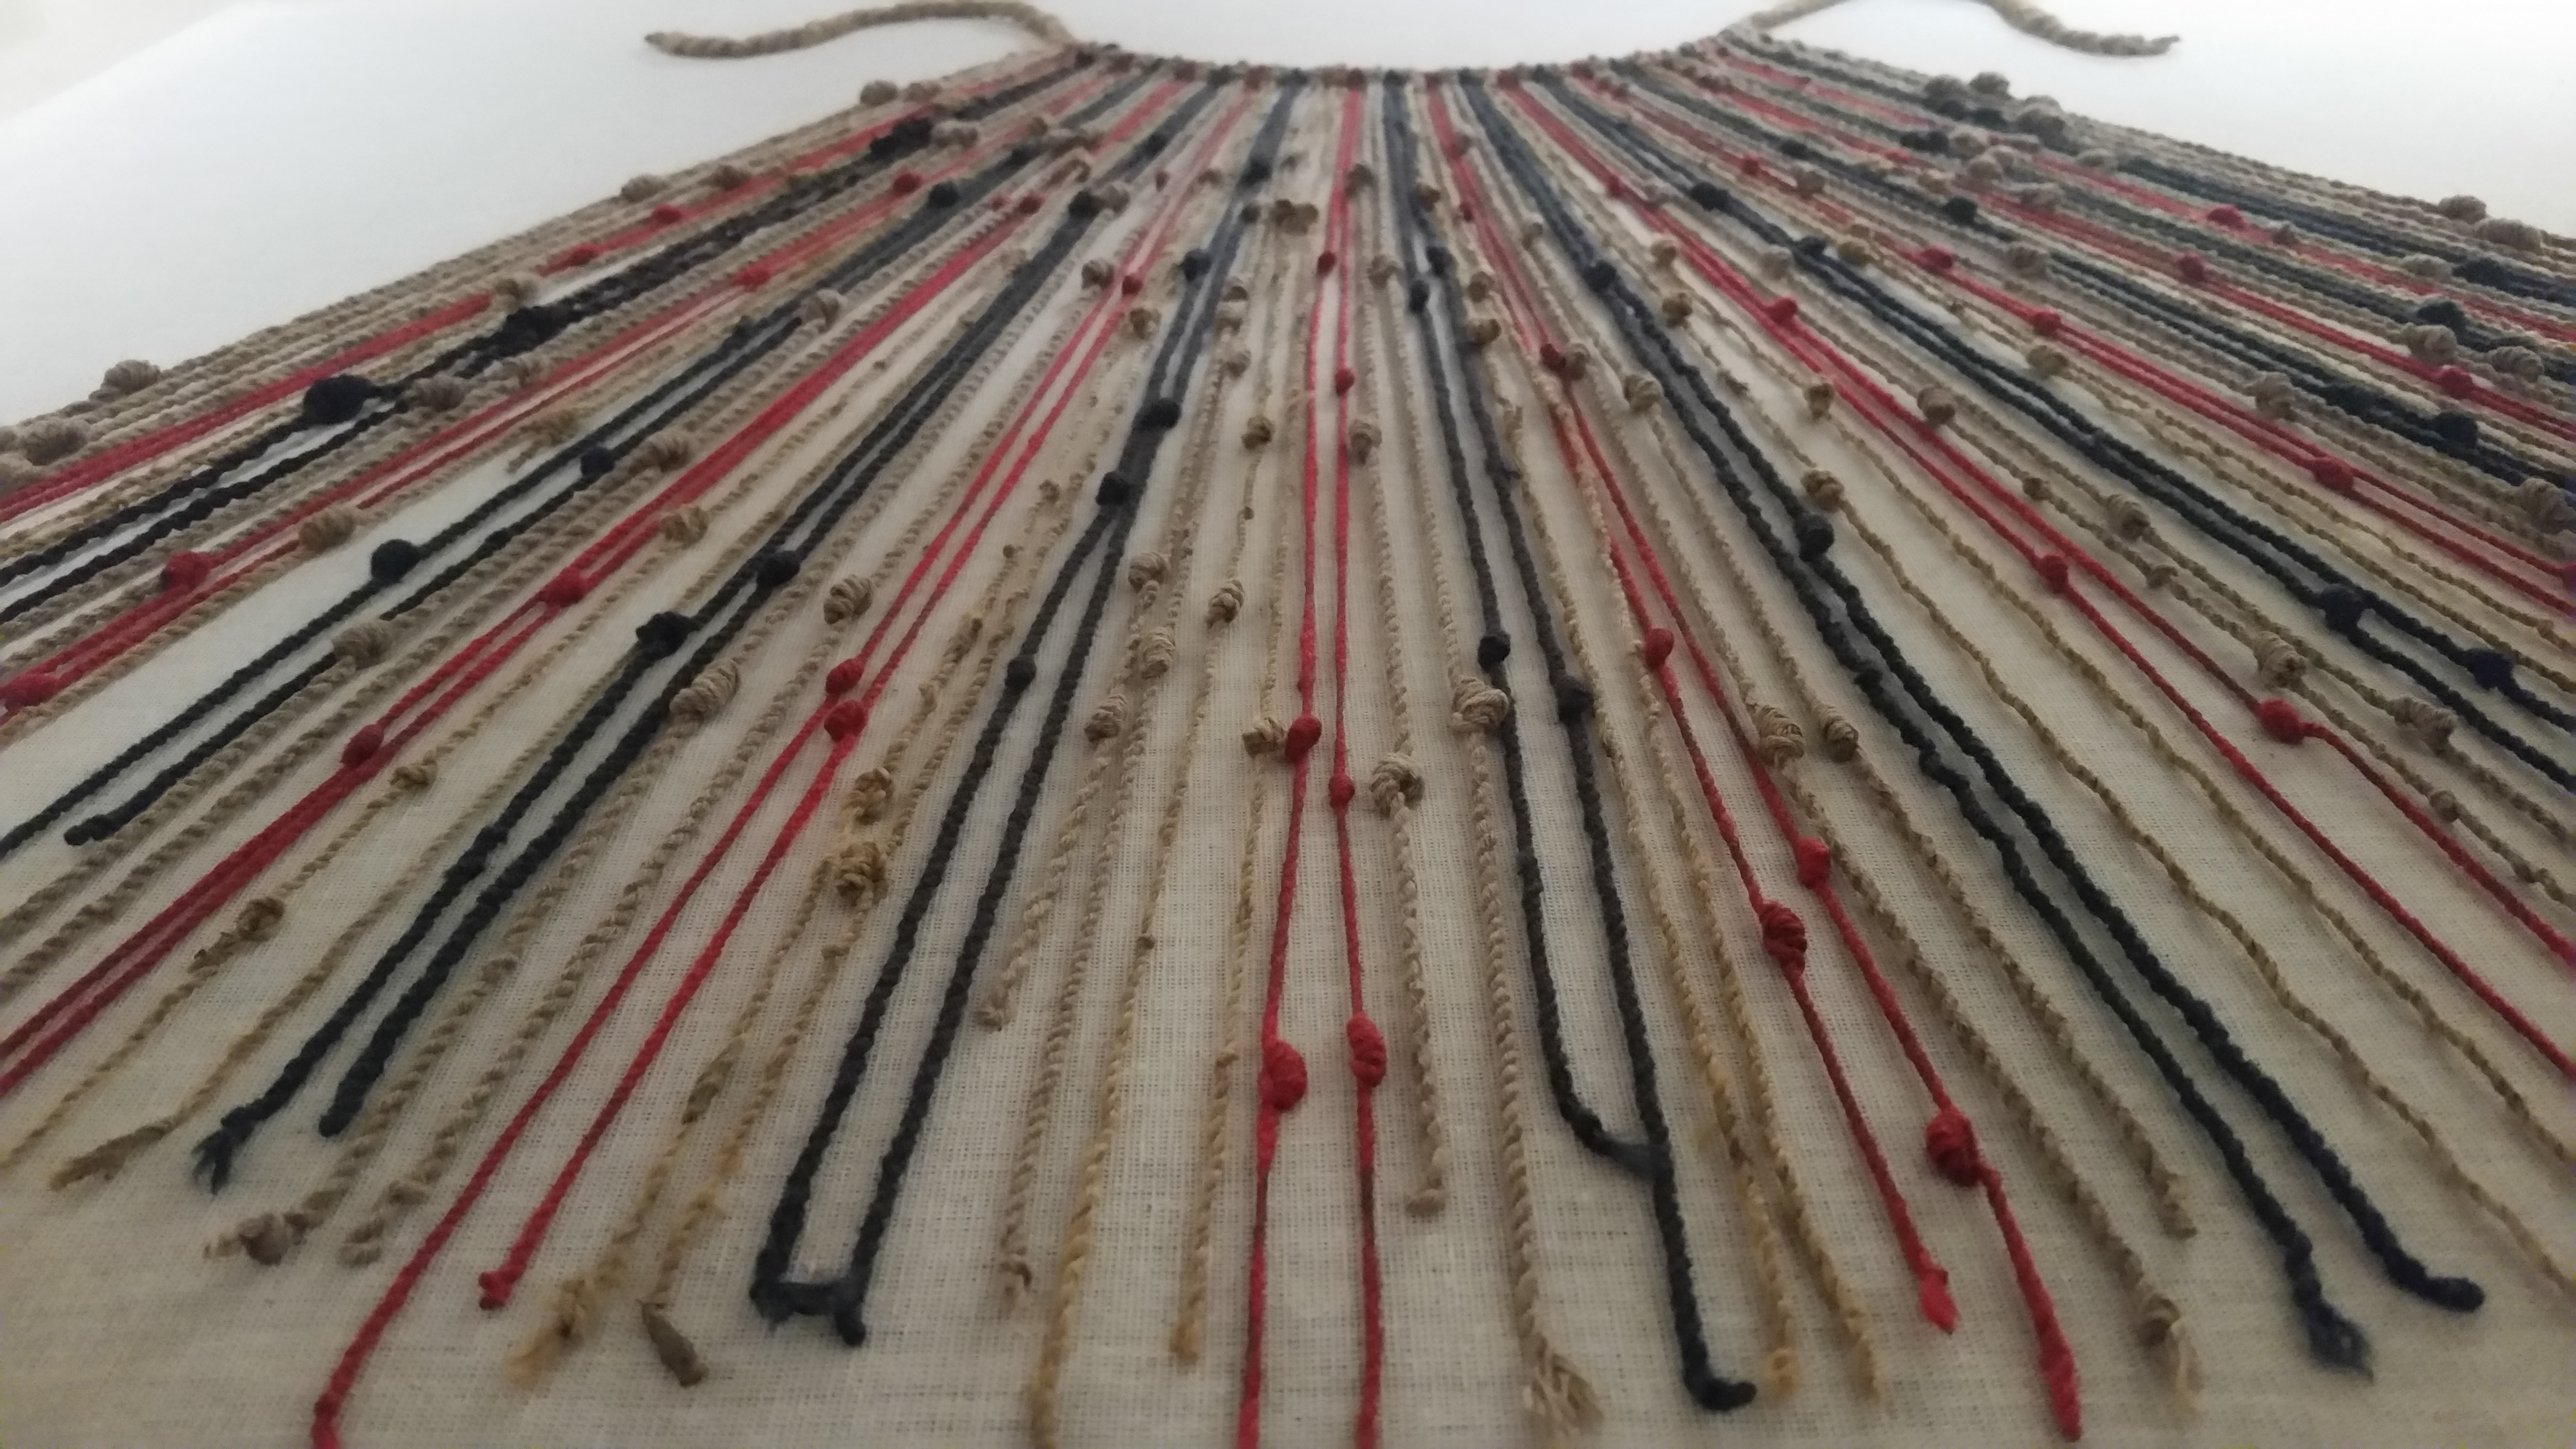
\includegraphics[width=\columnwidth]{../../../img/quipo.jpg}
\caption{\alert{Quipo}, Peru, 1300}
\end{figure}
}
\end{column}
\end{columns}
\end{frame}

\begin{frame}[label={sec:orga764b25}]{Primórdios da Computação: A Máquina de Anticítera}
\begin{columns}
\begin{column}{0.5\columnwidth}
\begin{figure}[htbp]
\centering
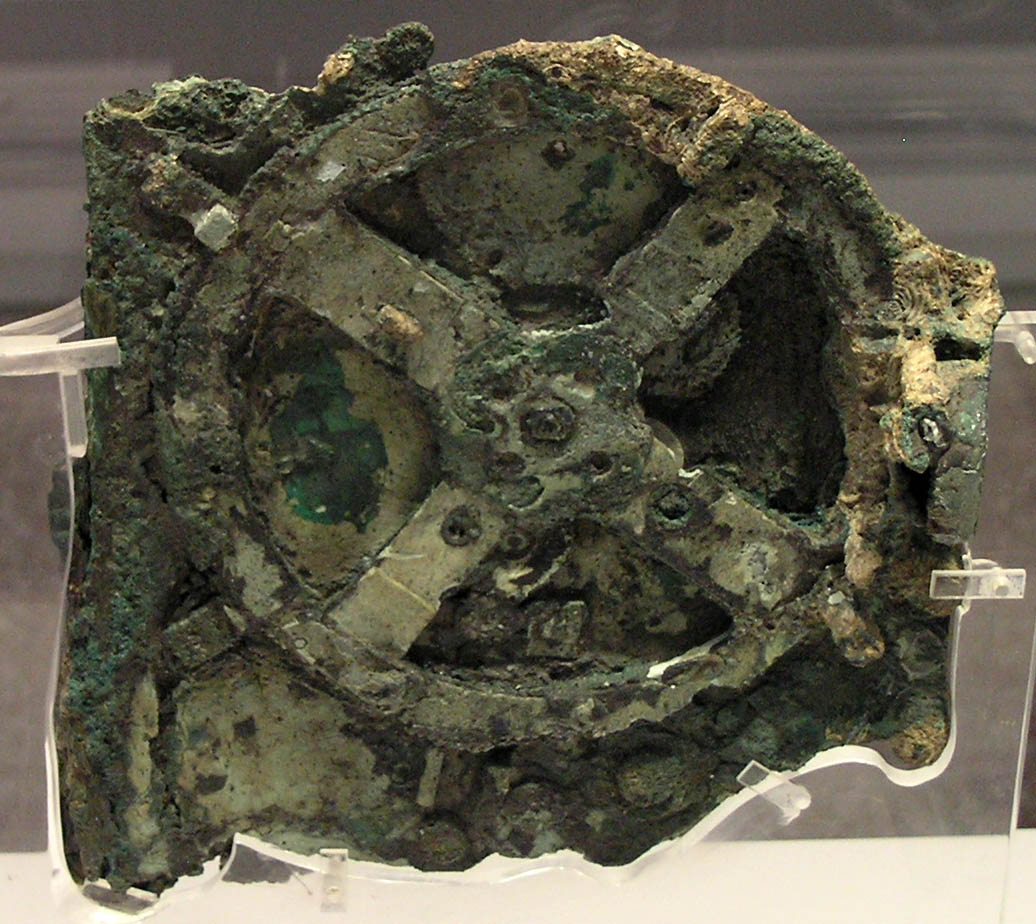
\includegraphics[width=.9\columnwidth]{../../../img/anticitera_frente.jpg}
\caption{Frente da \alert{Máquina de Anticítera}, \textasciitilde{}100 AC}
\end{figure}
\end{column}
\begin{column}{0.5\columnwidth}
\only<1>{
\begin{figure}[htbp]
\centering
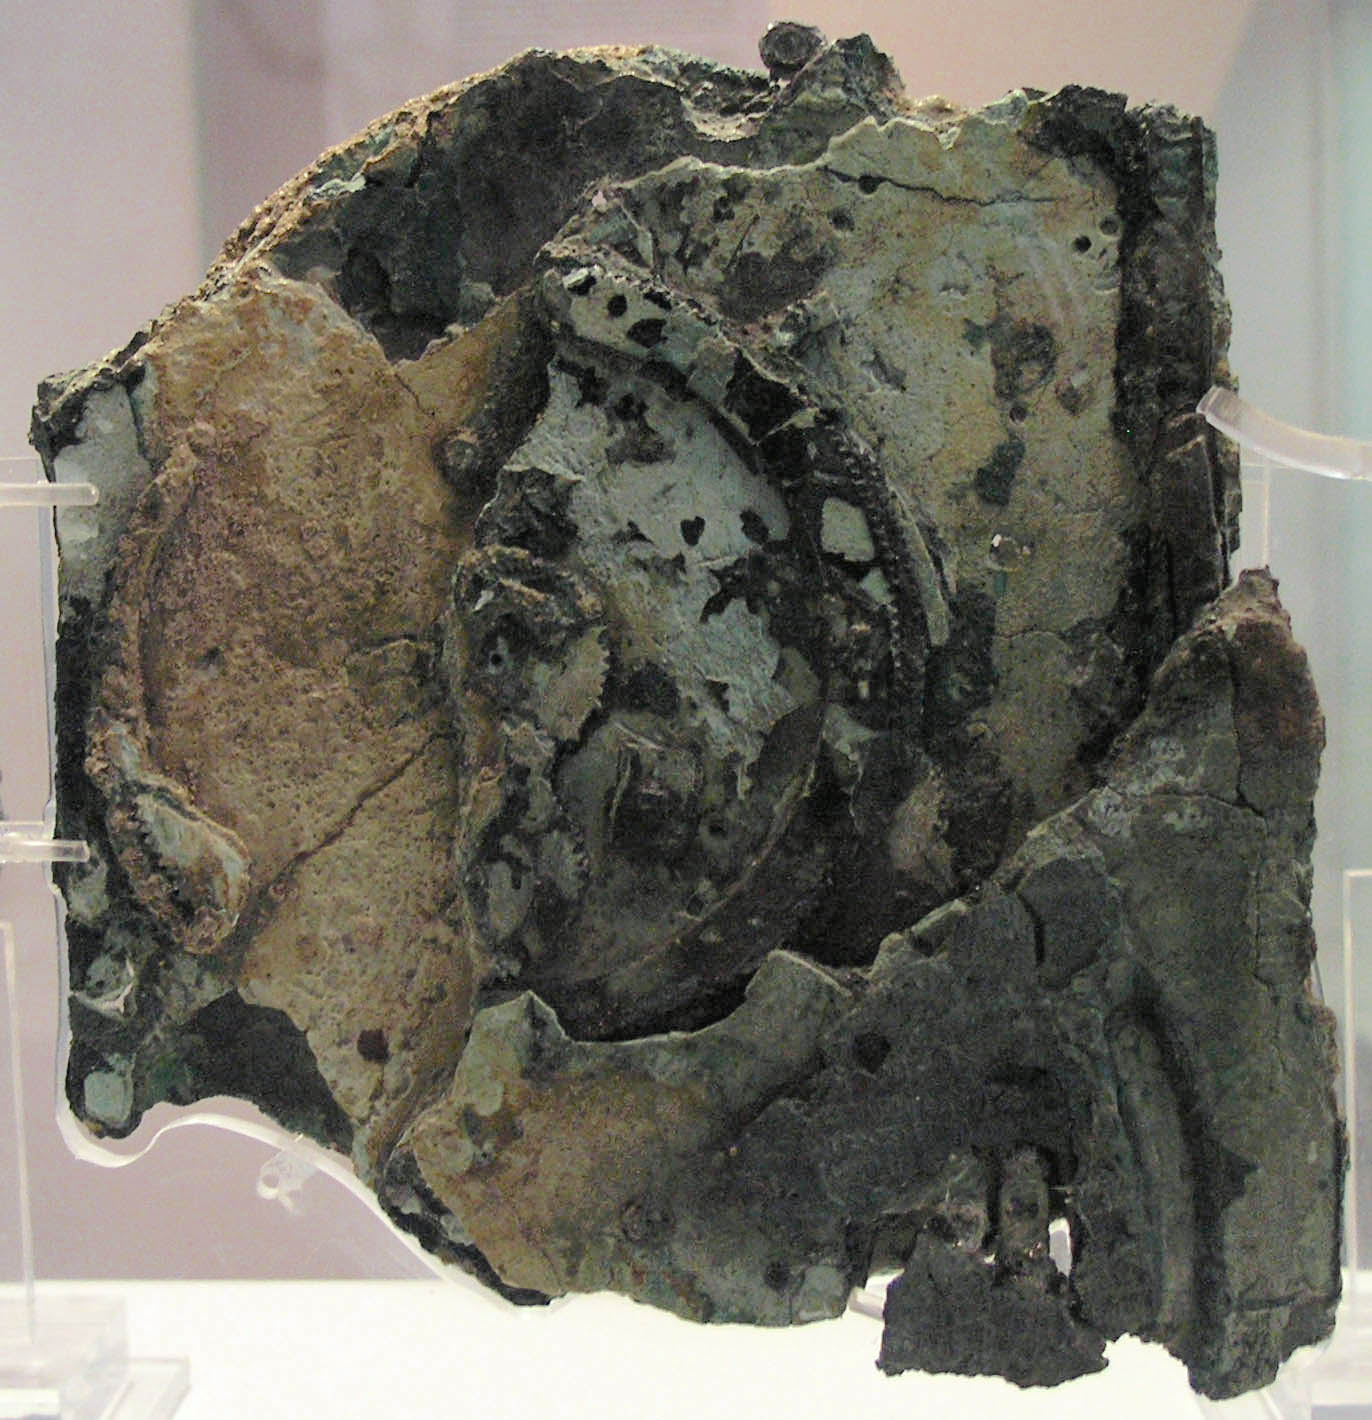
\includegraphics[width=.9\columnwidth]{../../../img/anticitera_tras.jpg}
\caption{Fundo da \alert{Máquina de Anticítera}, \textasciitilde{}100 AC}
\end{figure}
}

\only<2>{
\begin{figure}[htbp]
\centering
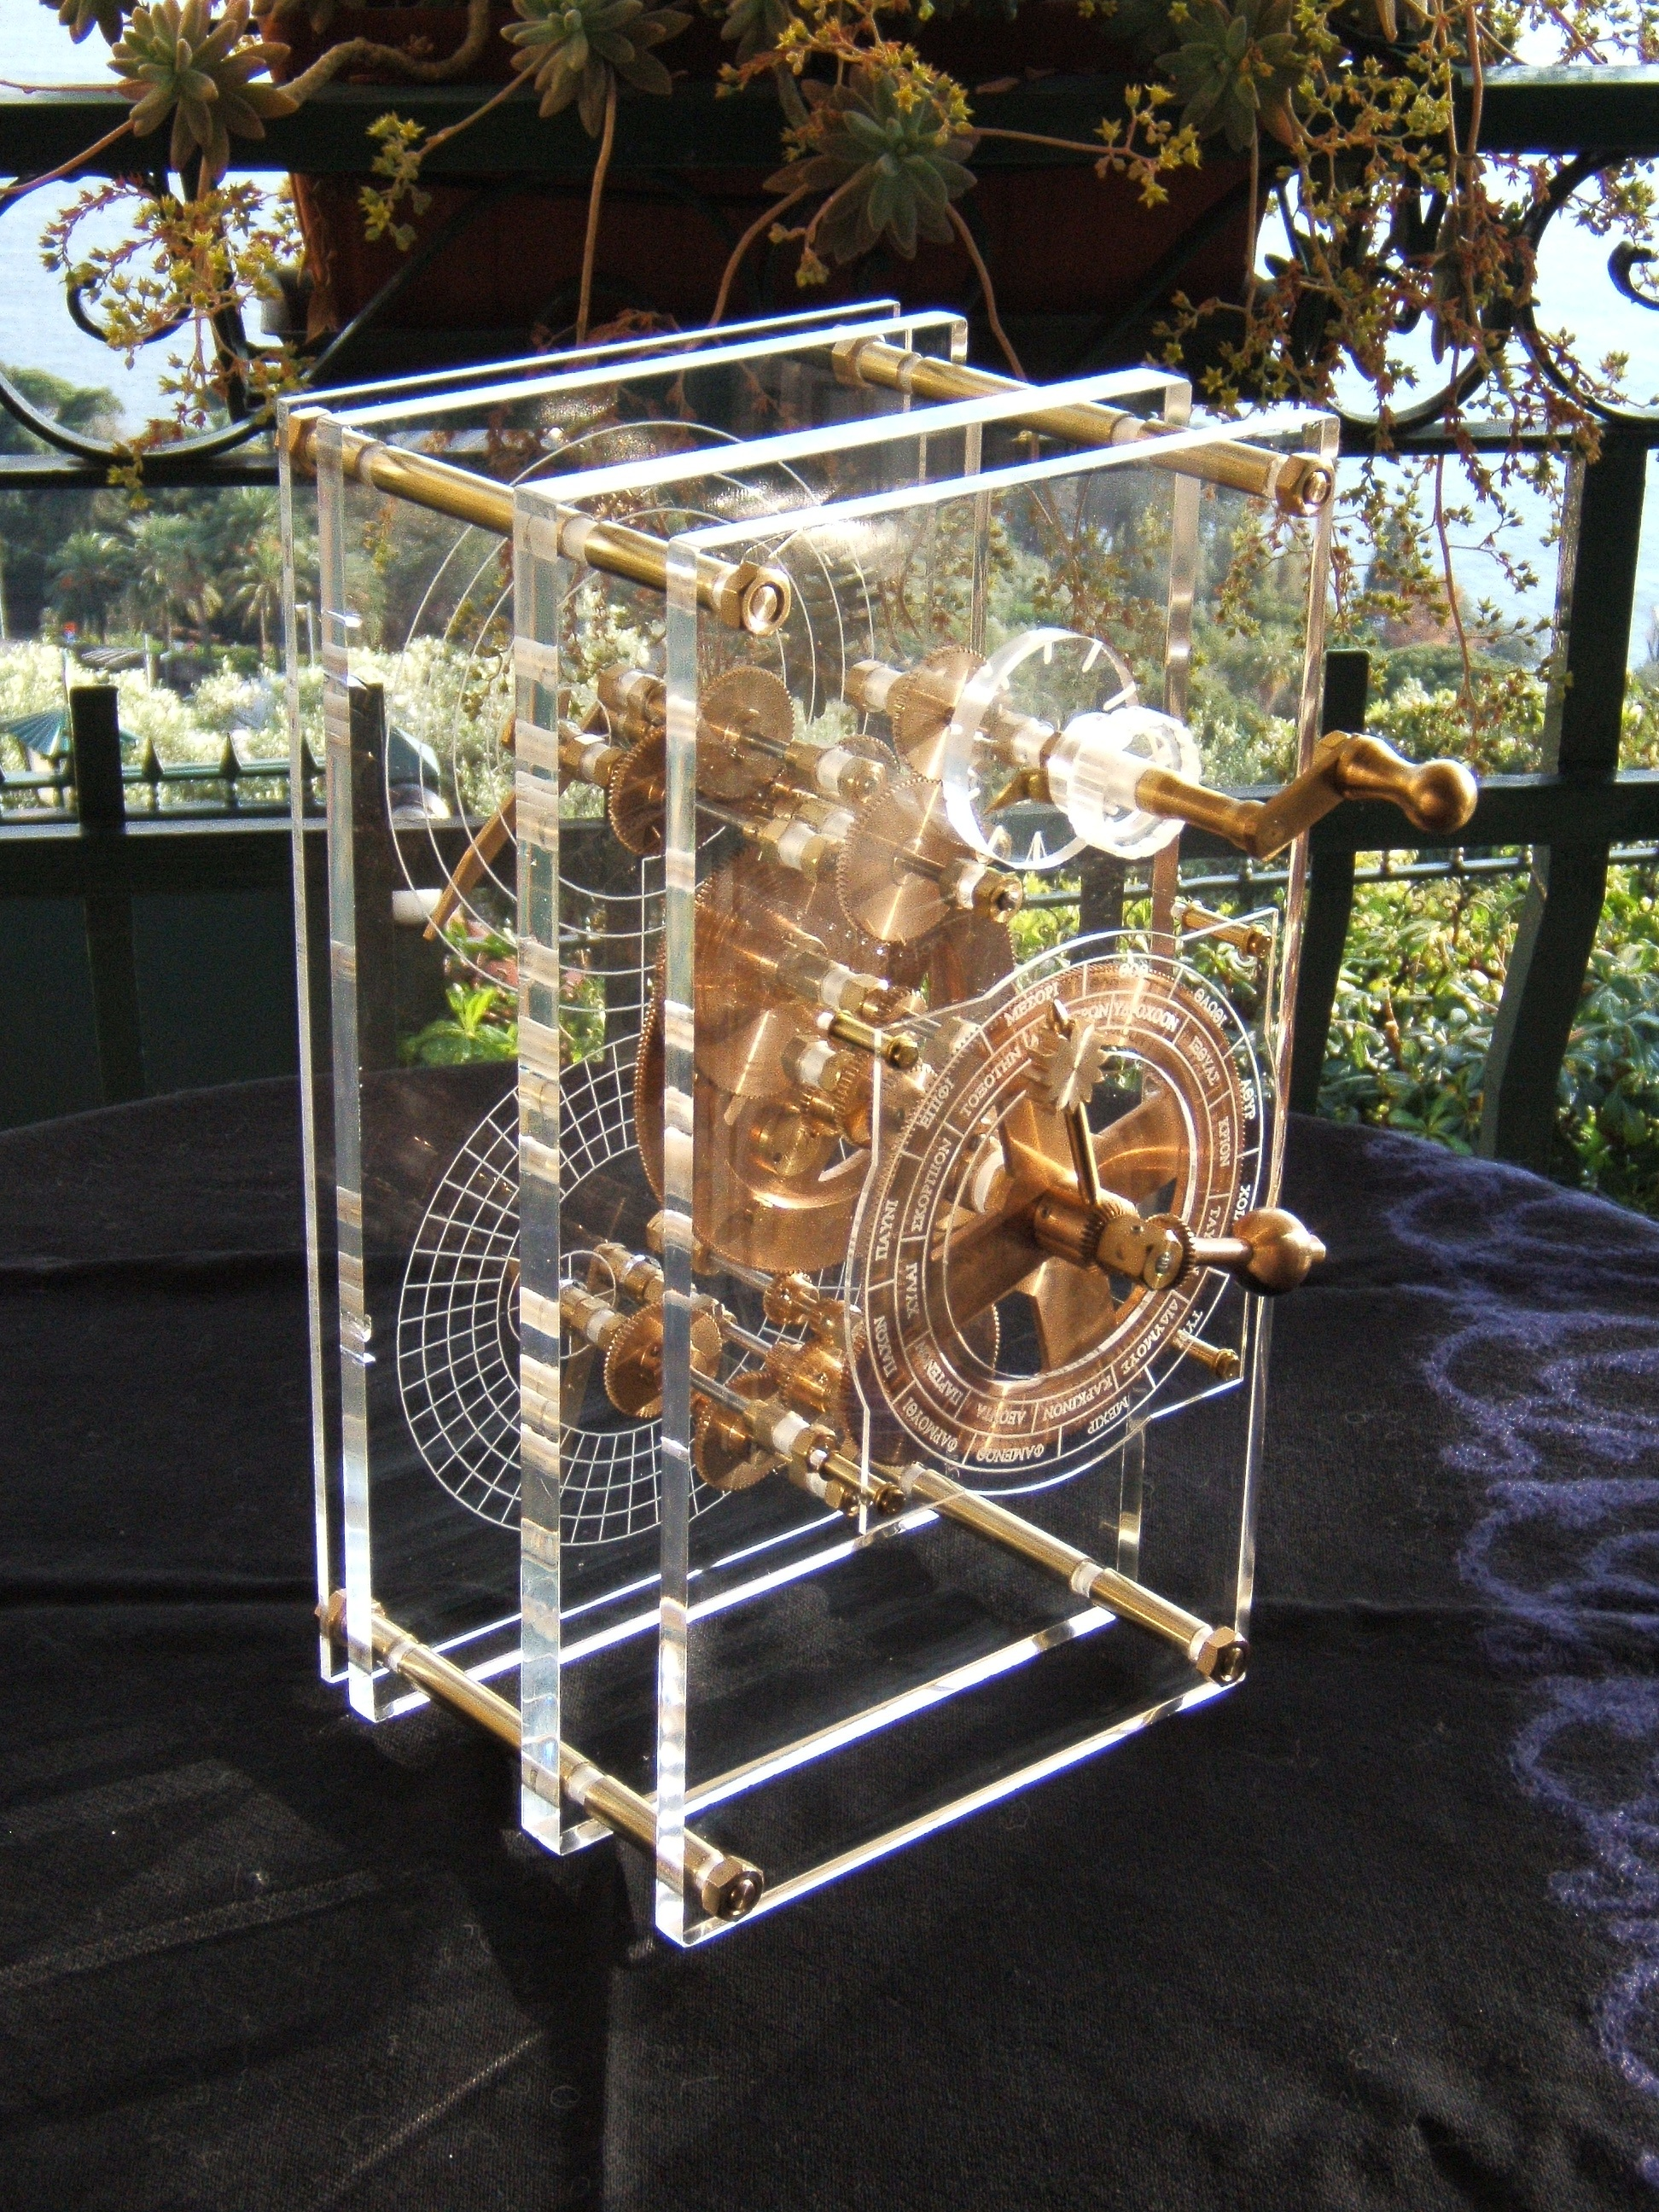
\includegraphics[width=.70\columnwidth]{../../../img/anticitera_2007.jpg}
\caption{Reprodução da \alert{Máquina de Anticítera}, 2007}
\end{figure}
}
\end{column}
\end{columns}
\end{frame}
\section{Computação Moderna}
\label{sec:org4d5d09f}
\begin{frame}[label={sec:orgbc8694a}]{Computação no Século 19}
\begin{columns}
\begin{column}{0.5\columnwidth}
\begin{block}{Linha do Tempo}
\begin{itemize}
\item Bonecos \alert{autômatos}: 1770
\item \visible<2->{Tear de Jacquard: 1804}
\item \visible<4->{Máquina \alert{Diferencial}: 1822}
\item \visible<7->{Máquina \alert{Analítica}: 1837}
\item \visible<9->{\alert{Programação}: \textasciitilde{}1837}
\item \visible<10->{Analisador Diferencial: 1878}
\end{itemize}
\end{block}
\end{column}

\begin{column}{0.5\columnwidth}
\only<1>{
\begin{figure}[htbp]
\centering
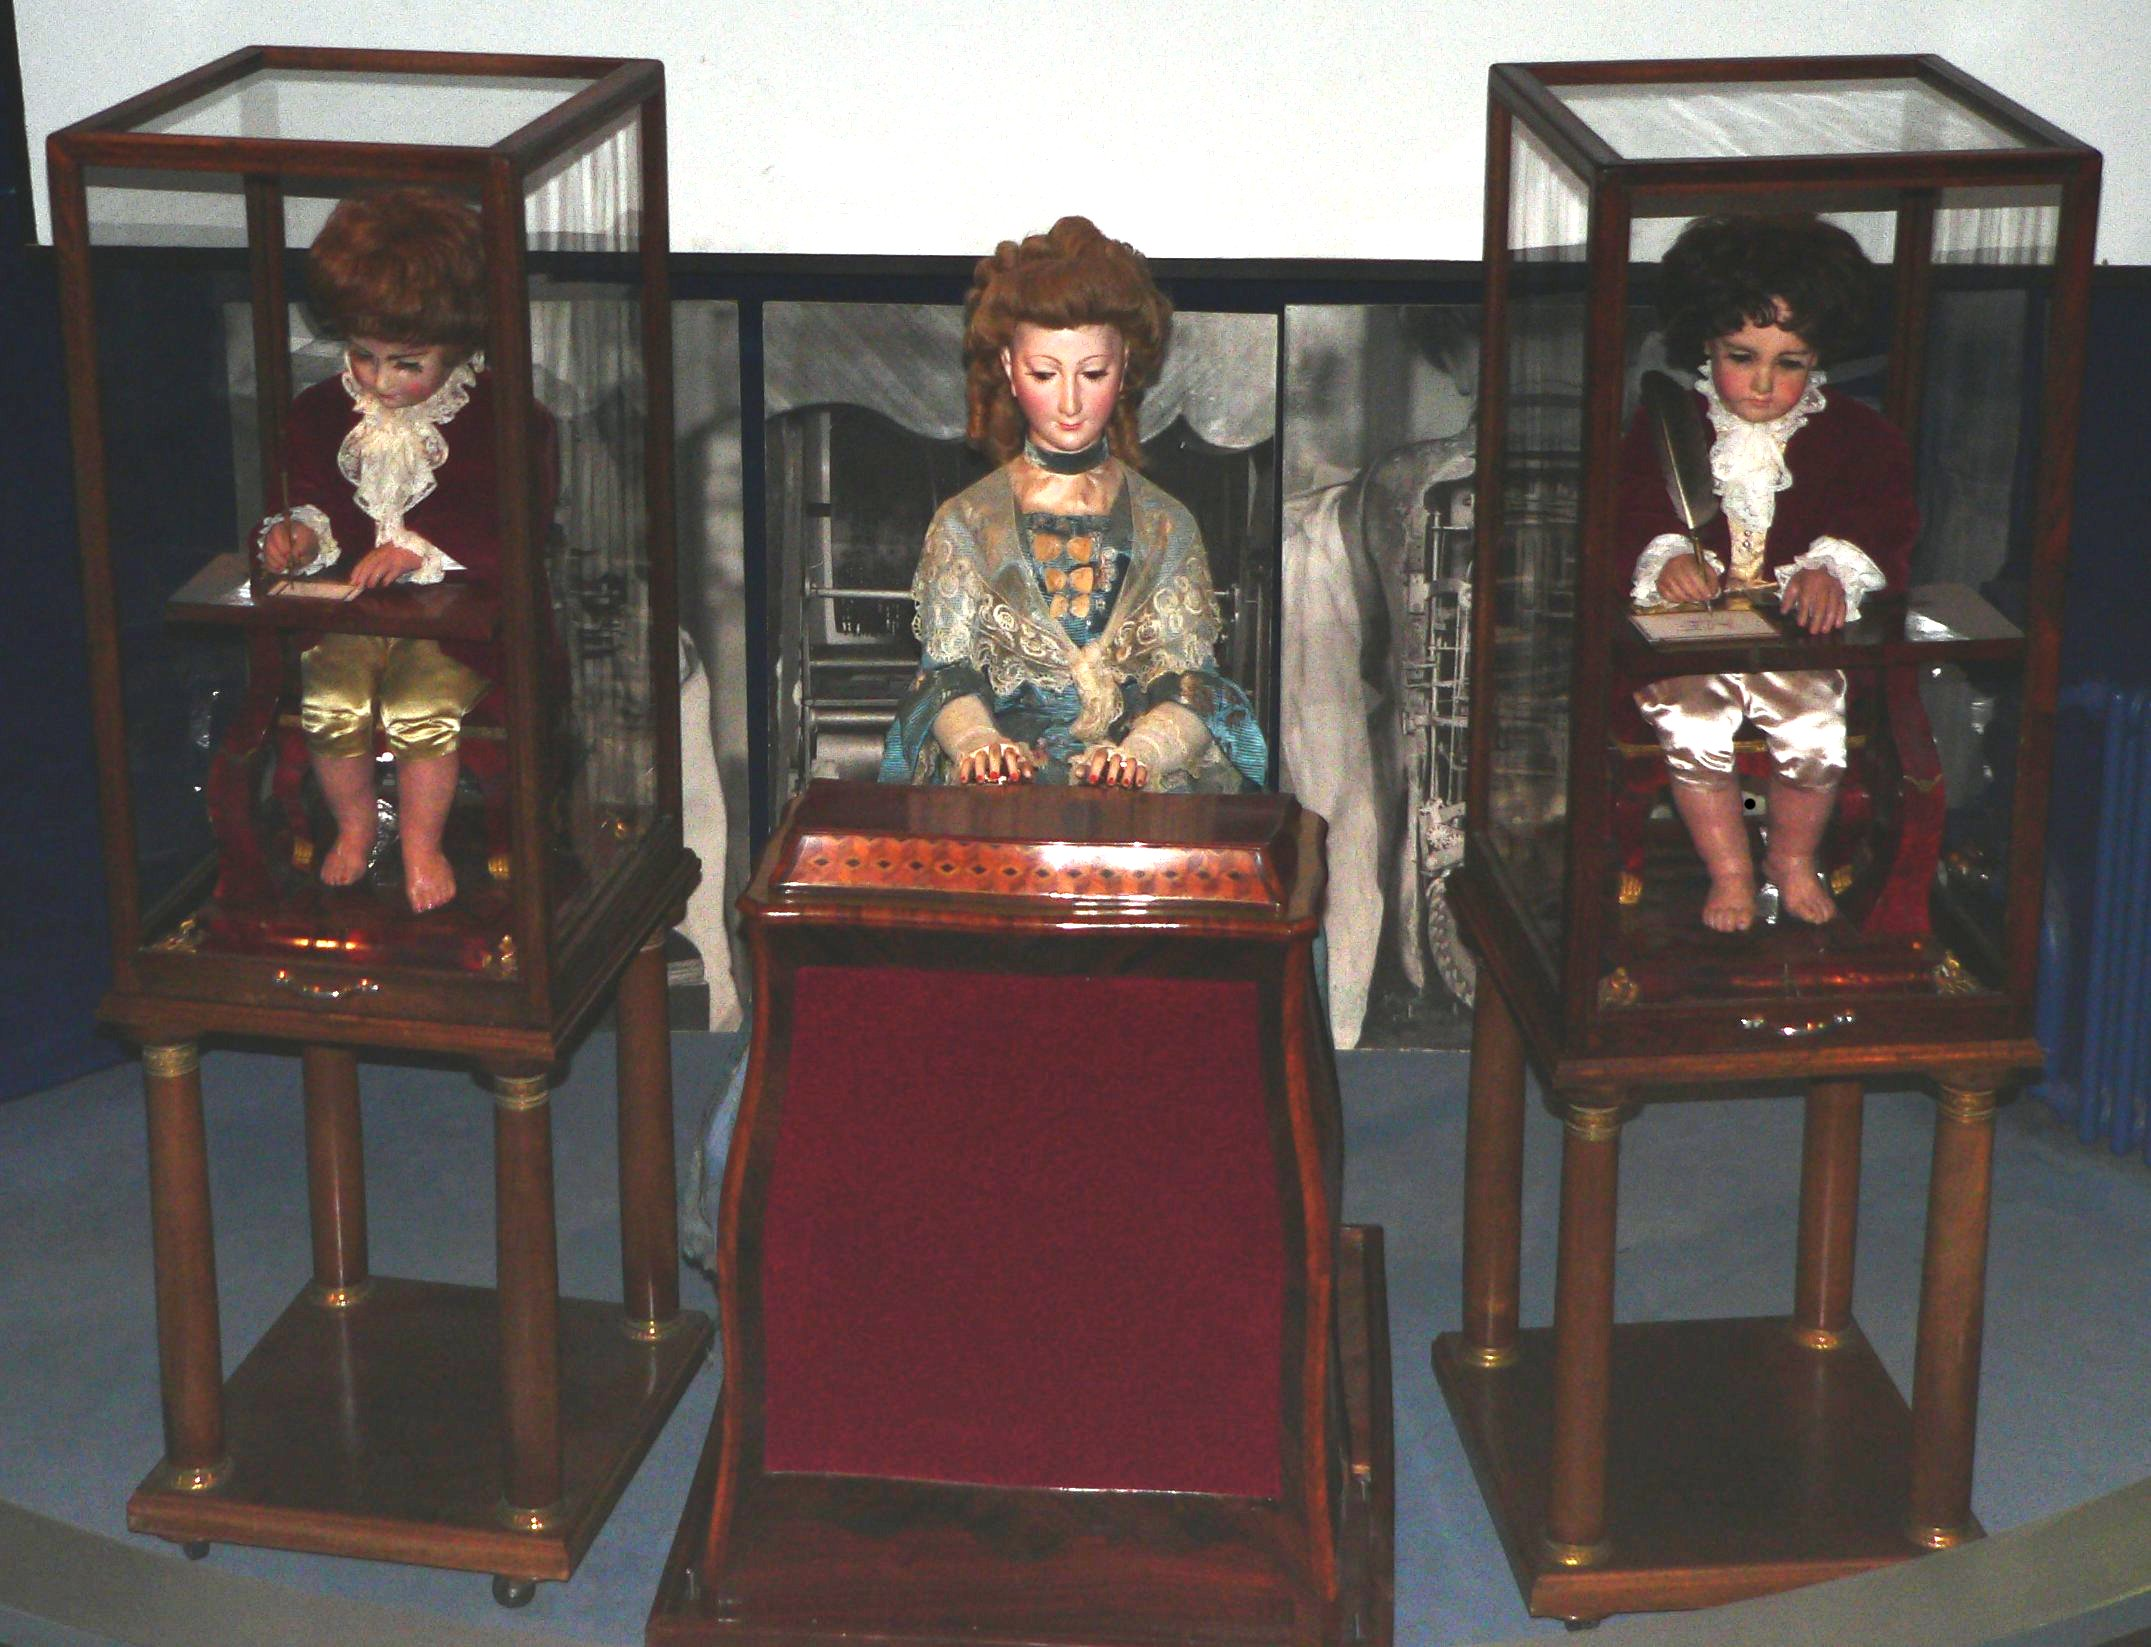
\includegraphics[width=\columnwidth]{../../../img/bonecos_automatos.jpg}
\caption{Bonecos escritores \alert{autômatos}}
\end{figure}
}

\only<2>{
\begin{figure}[htbp]
\centering
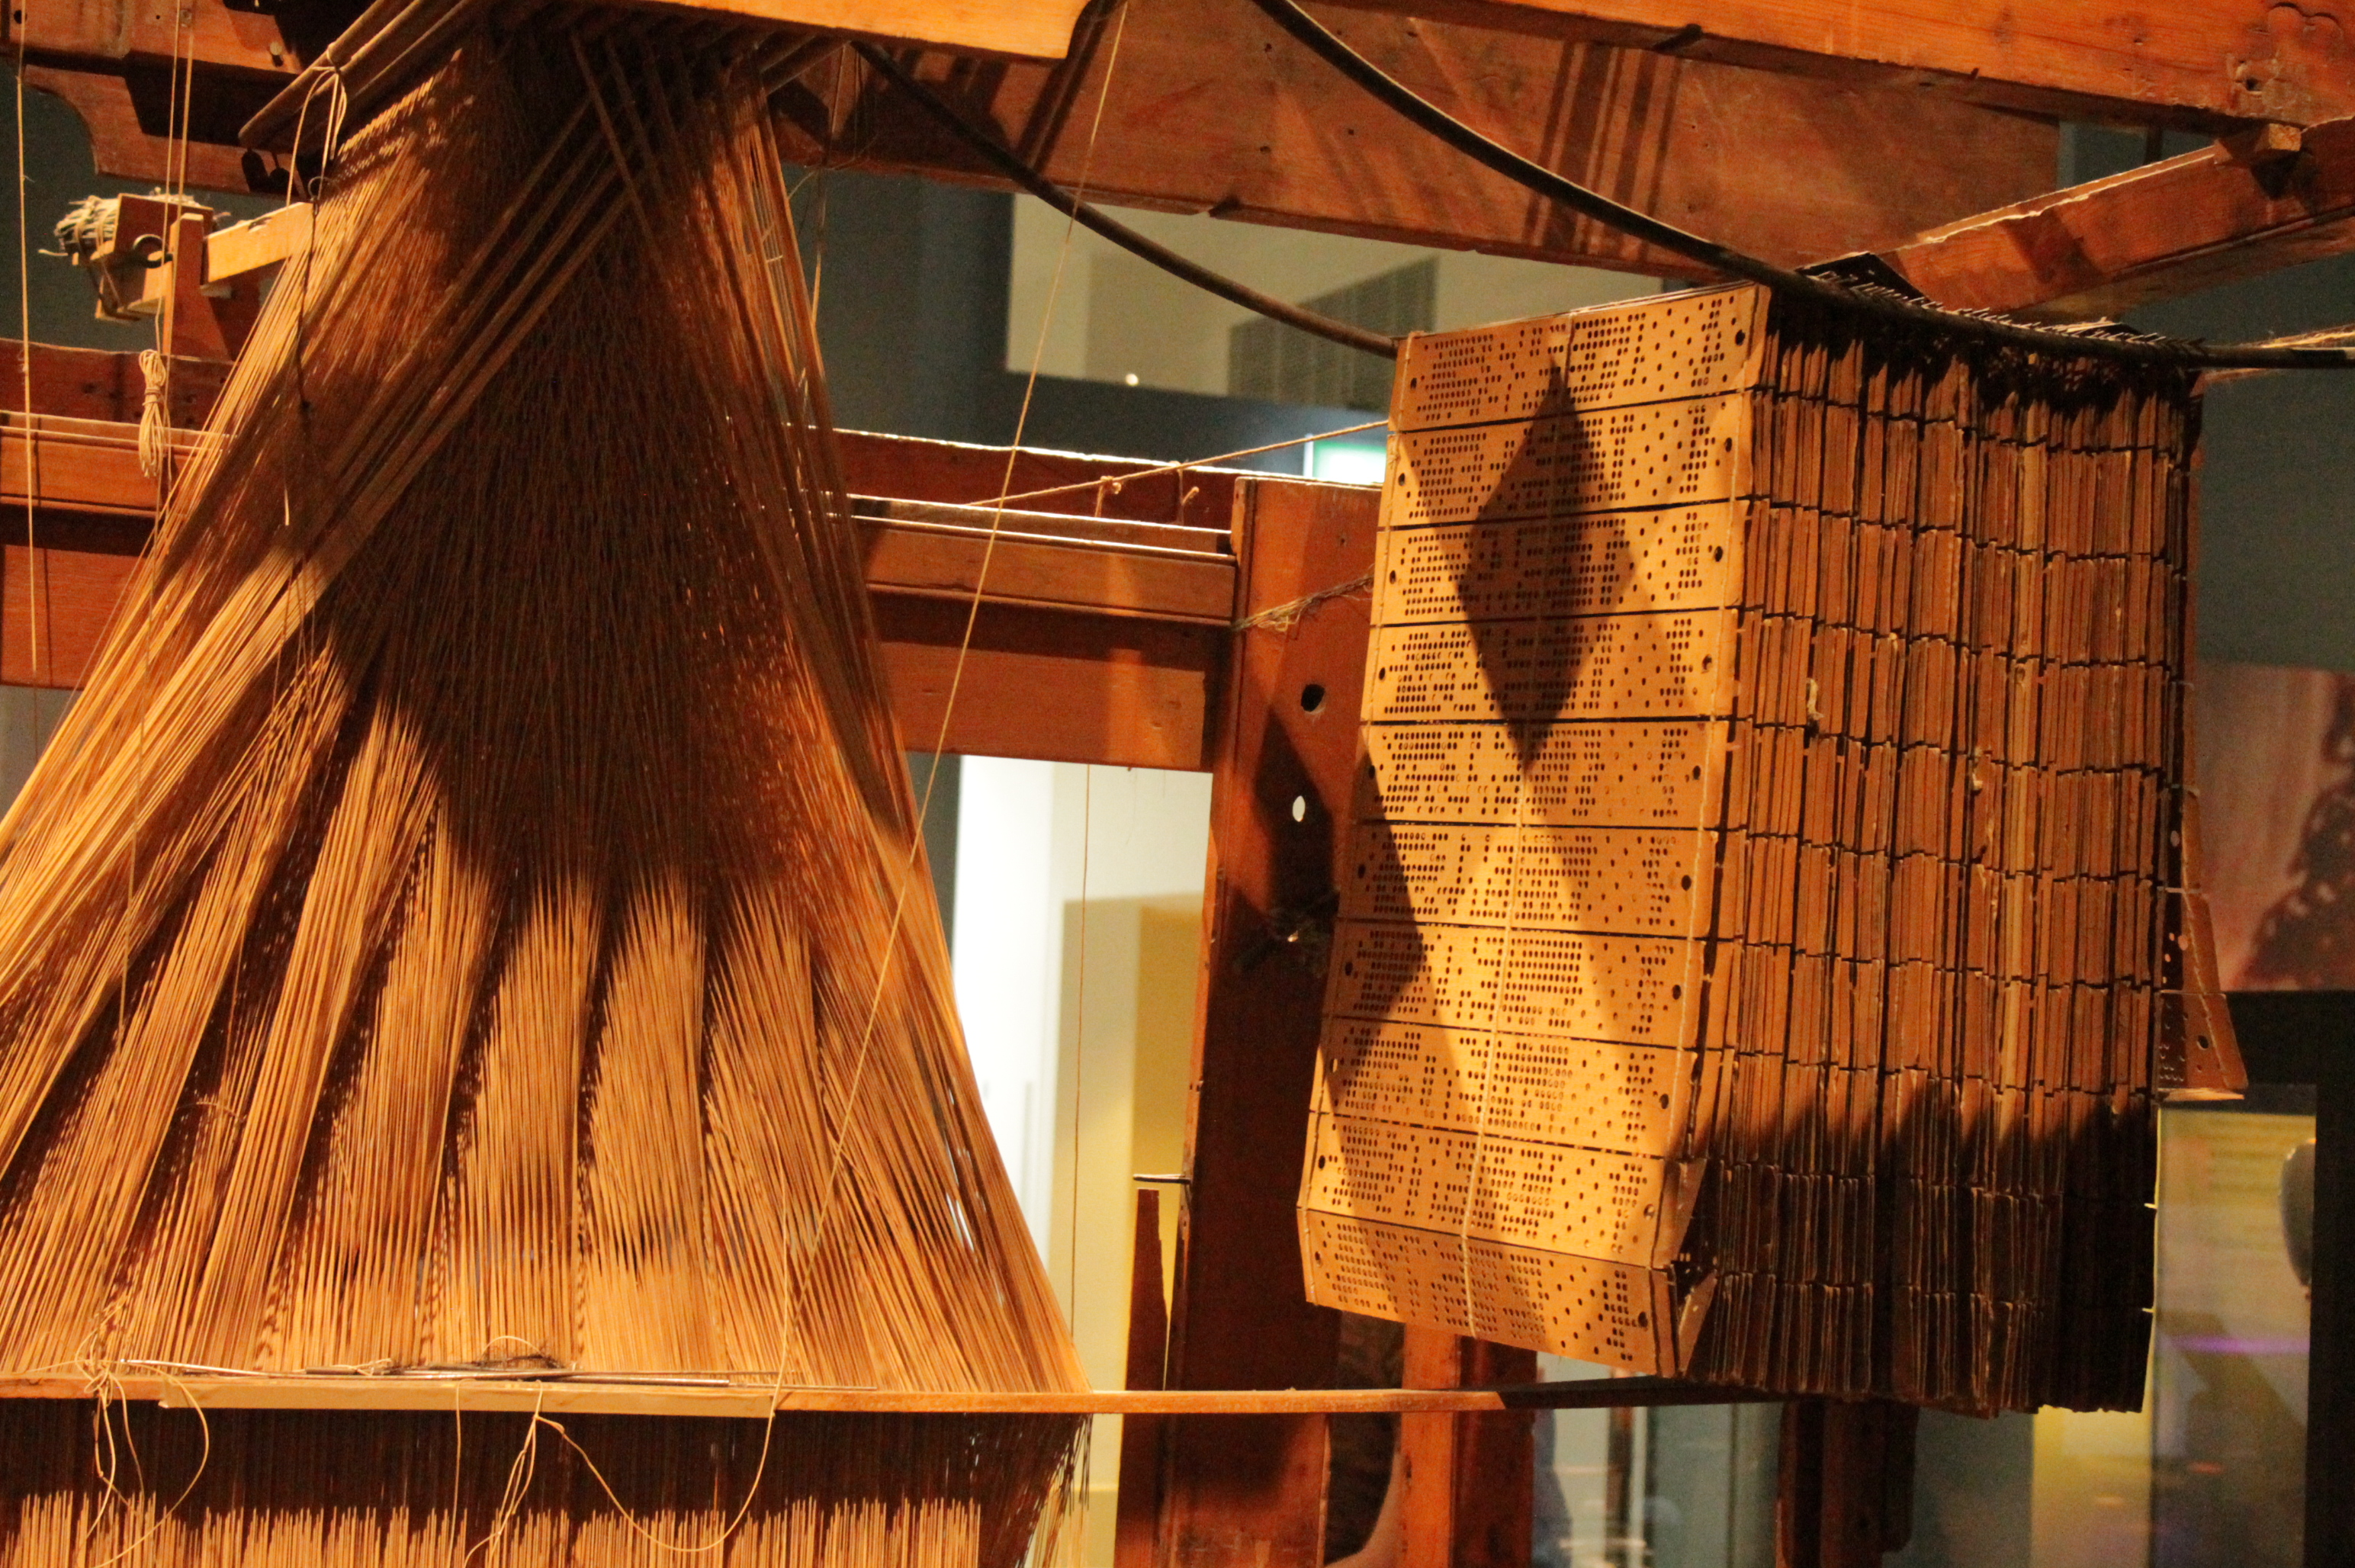
\includegraphics[width=1.0\columnwidth]{../../../img/tear_jacquard.jpg}
\caption{\alert{Tear de Jacquard}, Museu Nacional da Escócia}
\end{figure}
}

\only<3>{
\begin{figure}[htbp]
\centering
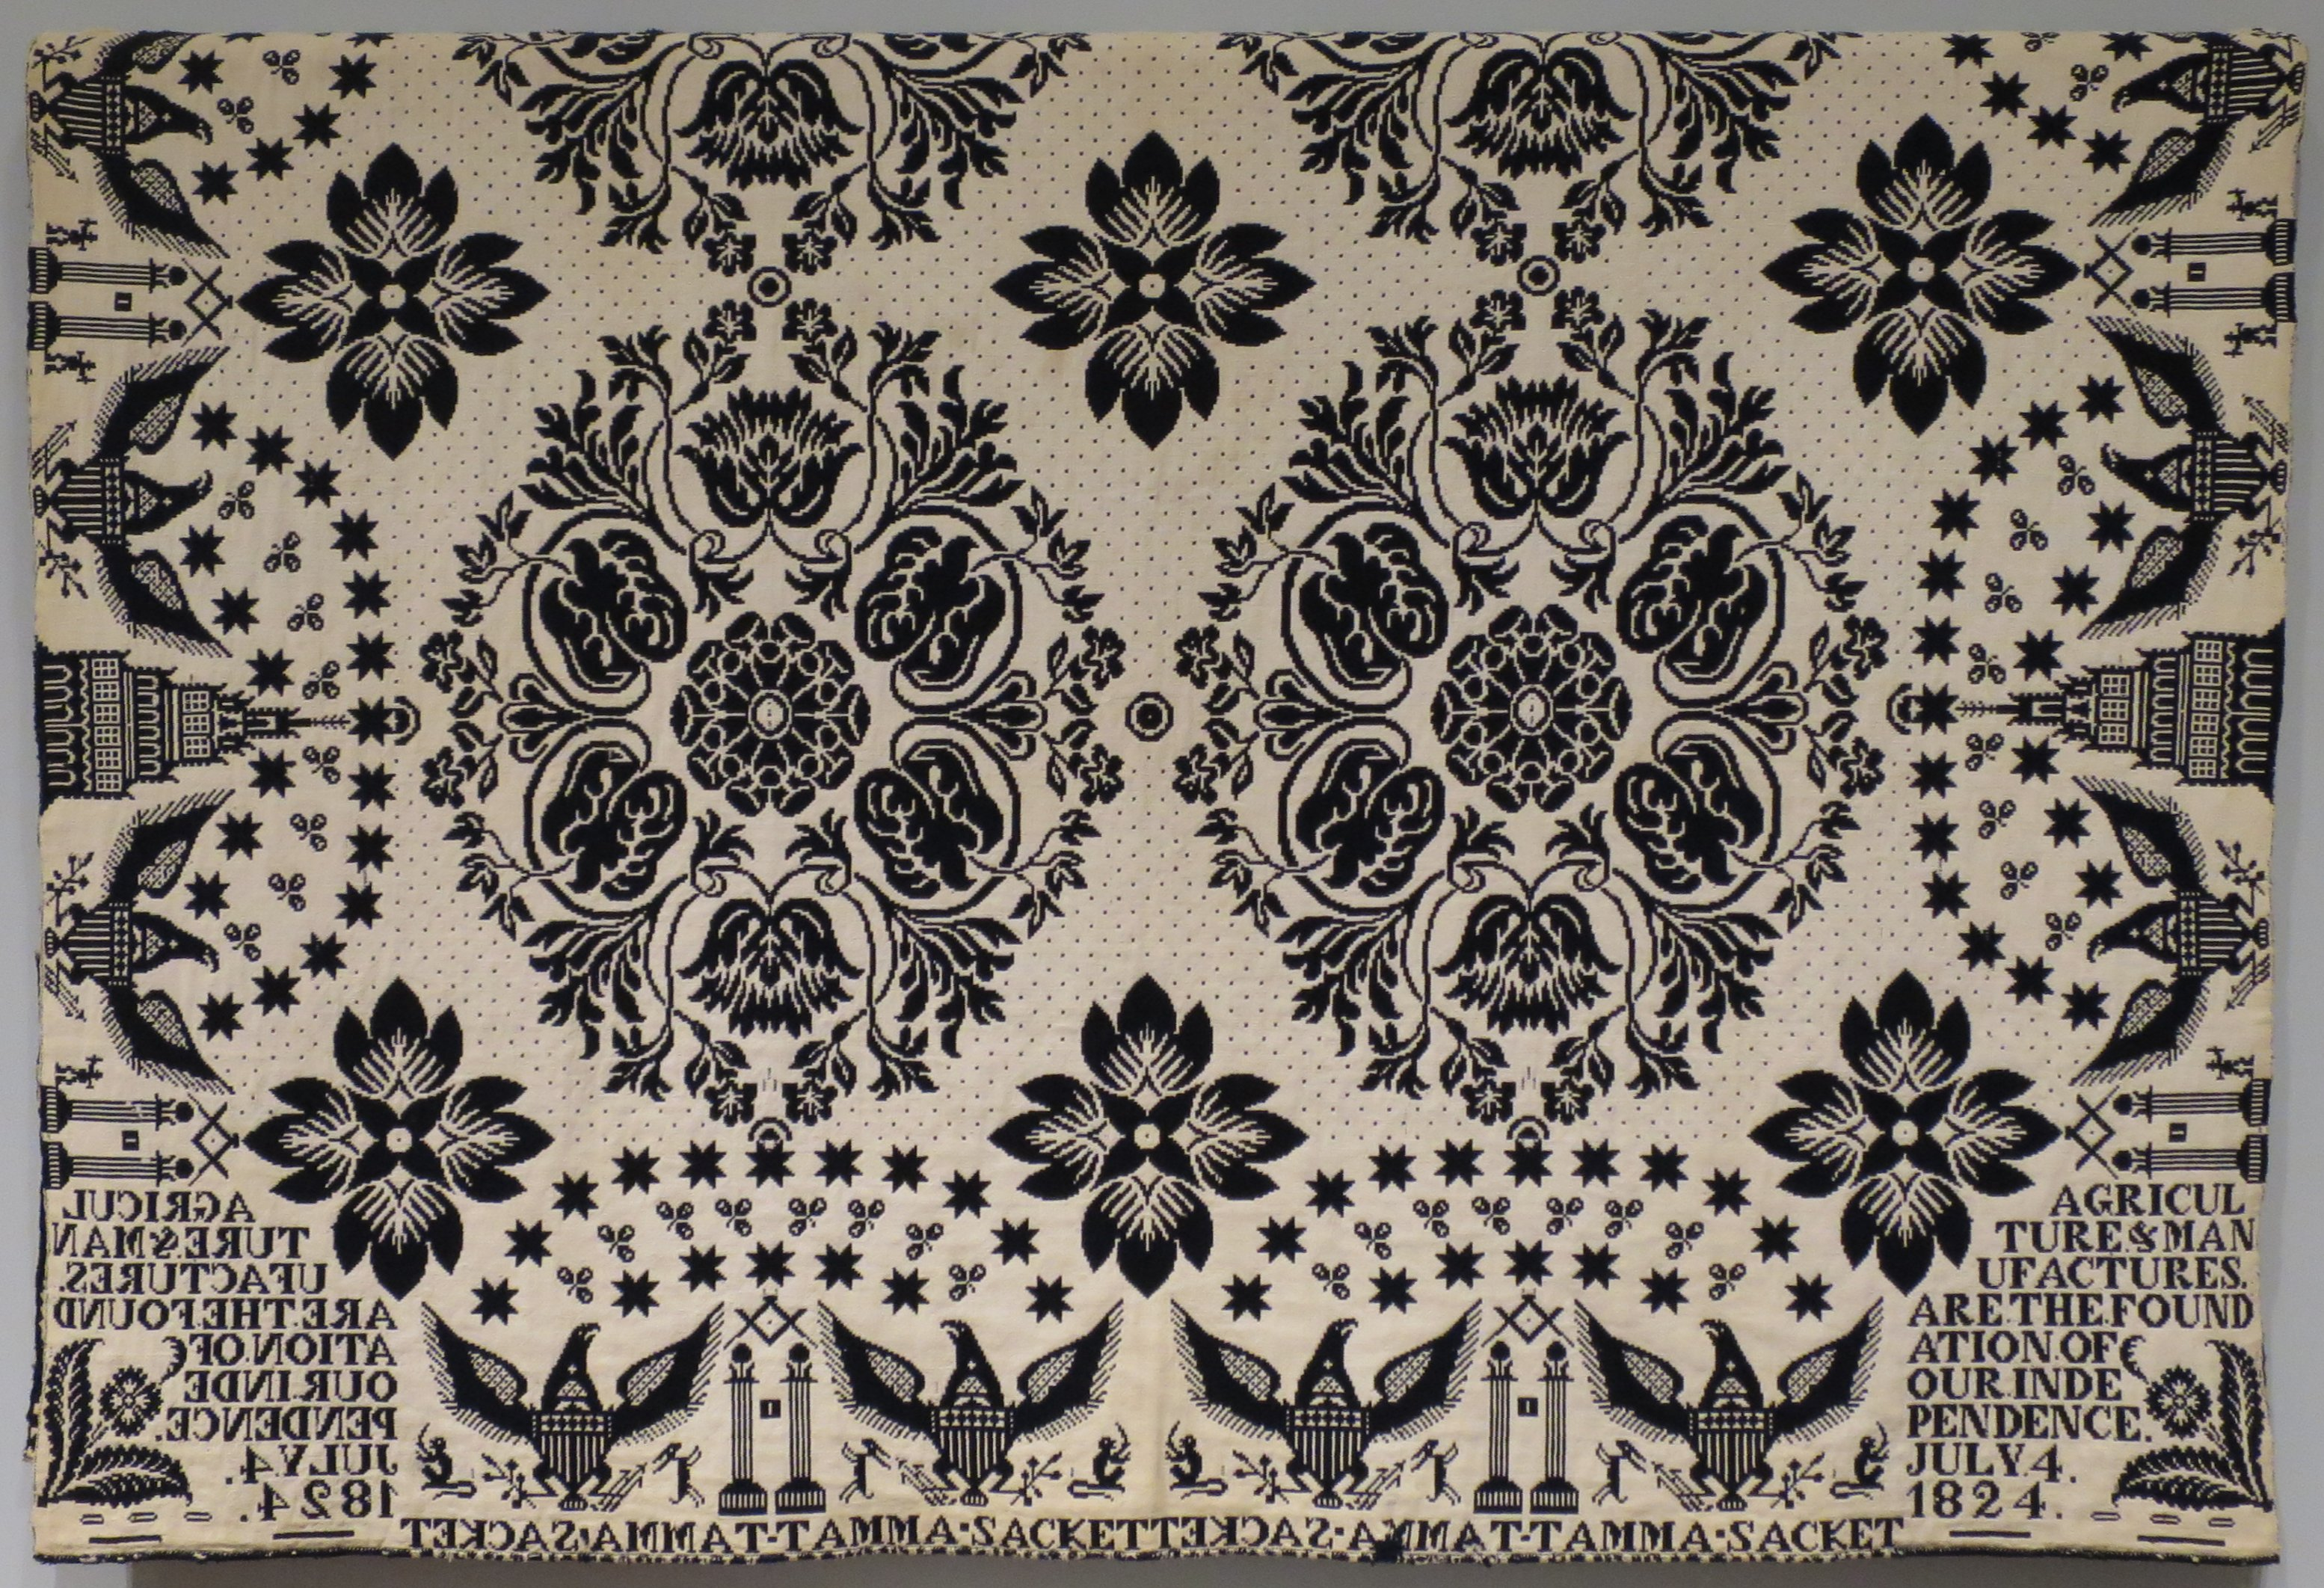
\includegraphics[width=1.0\columnwidth]{../../../img/tecido_tear_jacquard.jpg}
\caption{Tecido feito no \alert{Tear de Jacquard}}
\end{figure}
}

\only<4>{
\begin{figure}[htbp]
\centering
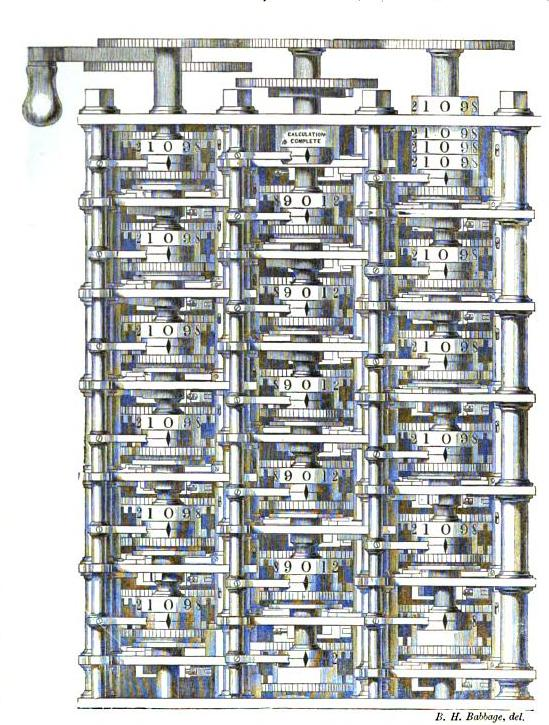
\includegraphics[width=0.62\columnwidth]{../../../img/diferencial_0.jpg}
\caption{\alert{Máquina Diferencial} de Charles Babbage}
\end{figure}
}

\only<5>{
\begin{figure}[htbp]
\centering
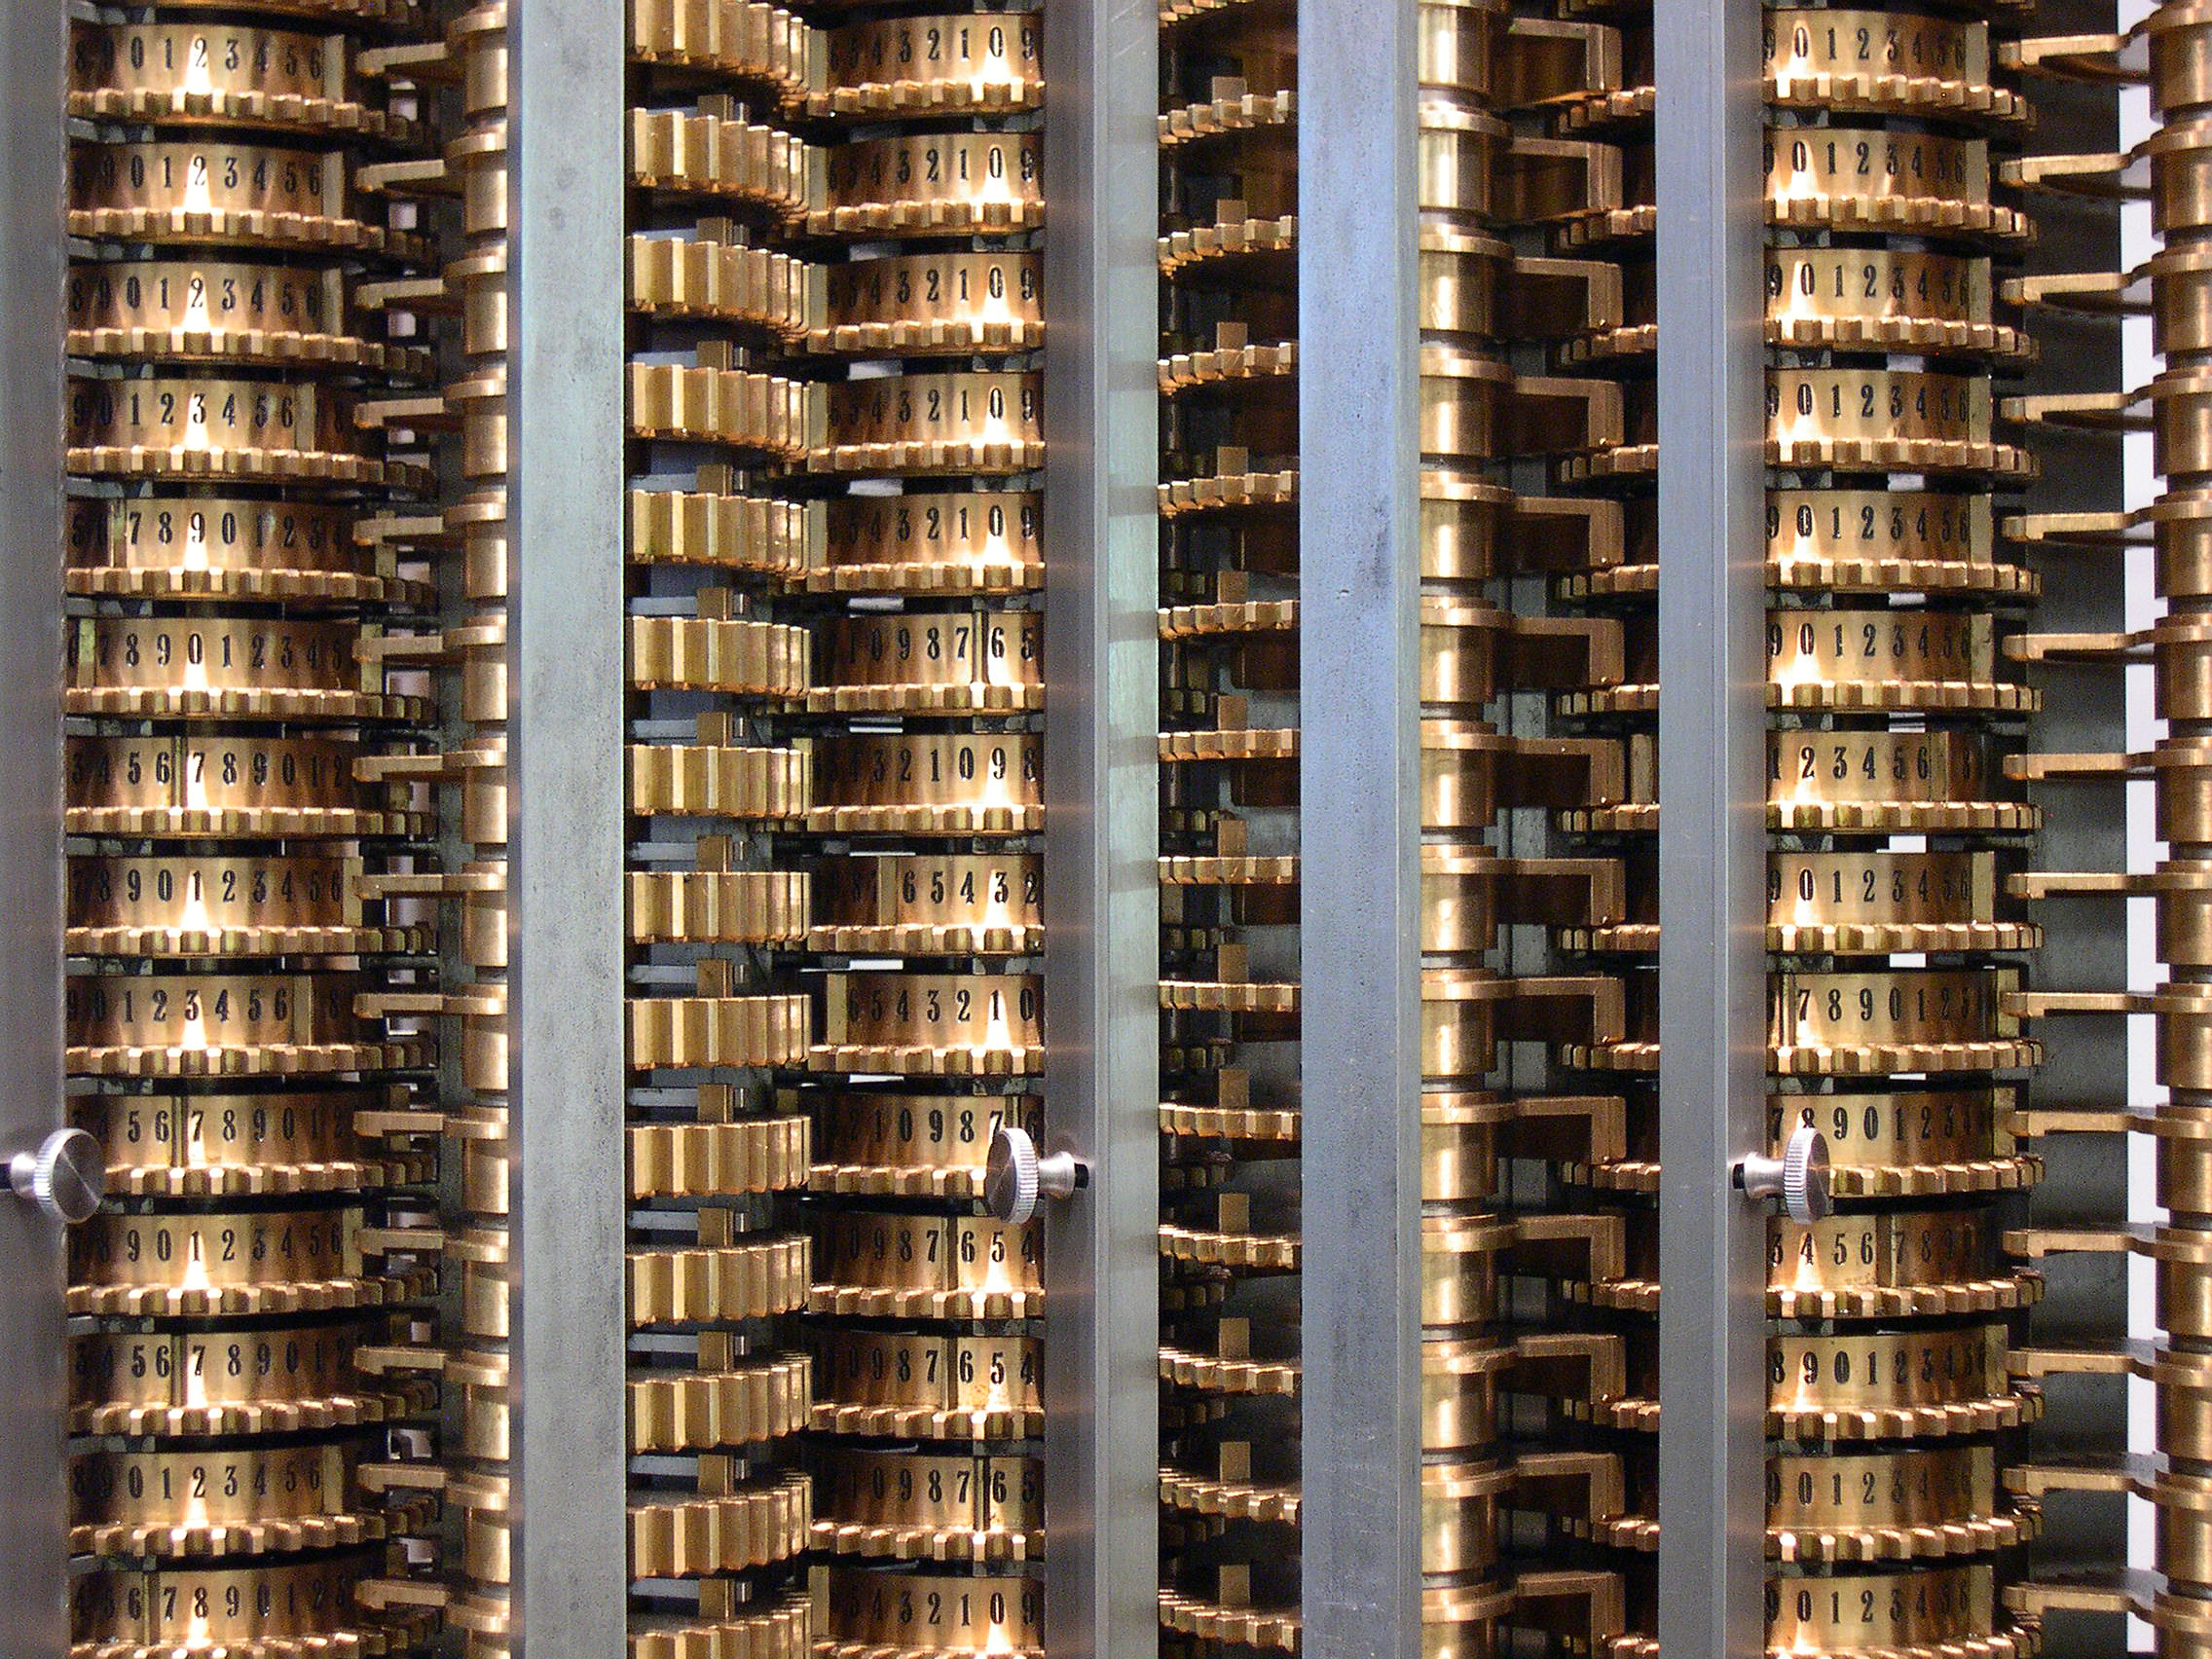
\includegraphics[width=\columnwidth]{../../../img/diferencial_1.jpg}
\caption{\alert{Máquina Diferencial} de Charles Babbage}
\end{figure}
}

\only<6>{
\begin{figure}[htbp]
\centering
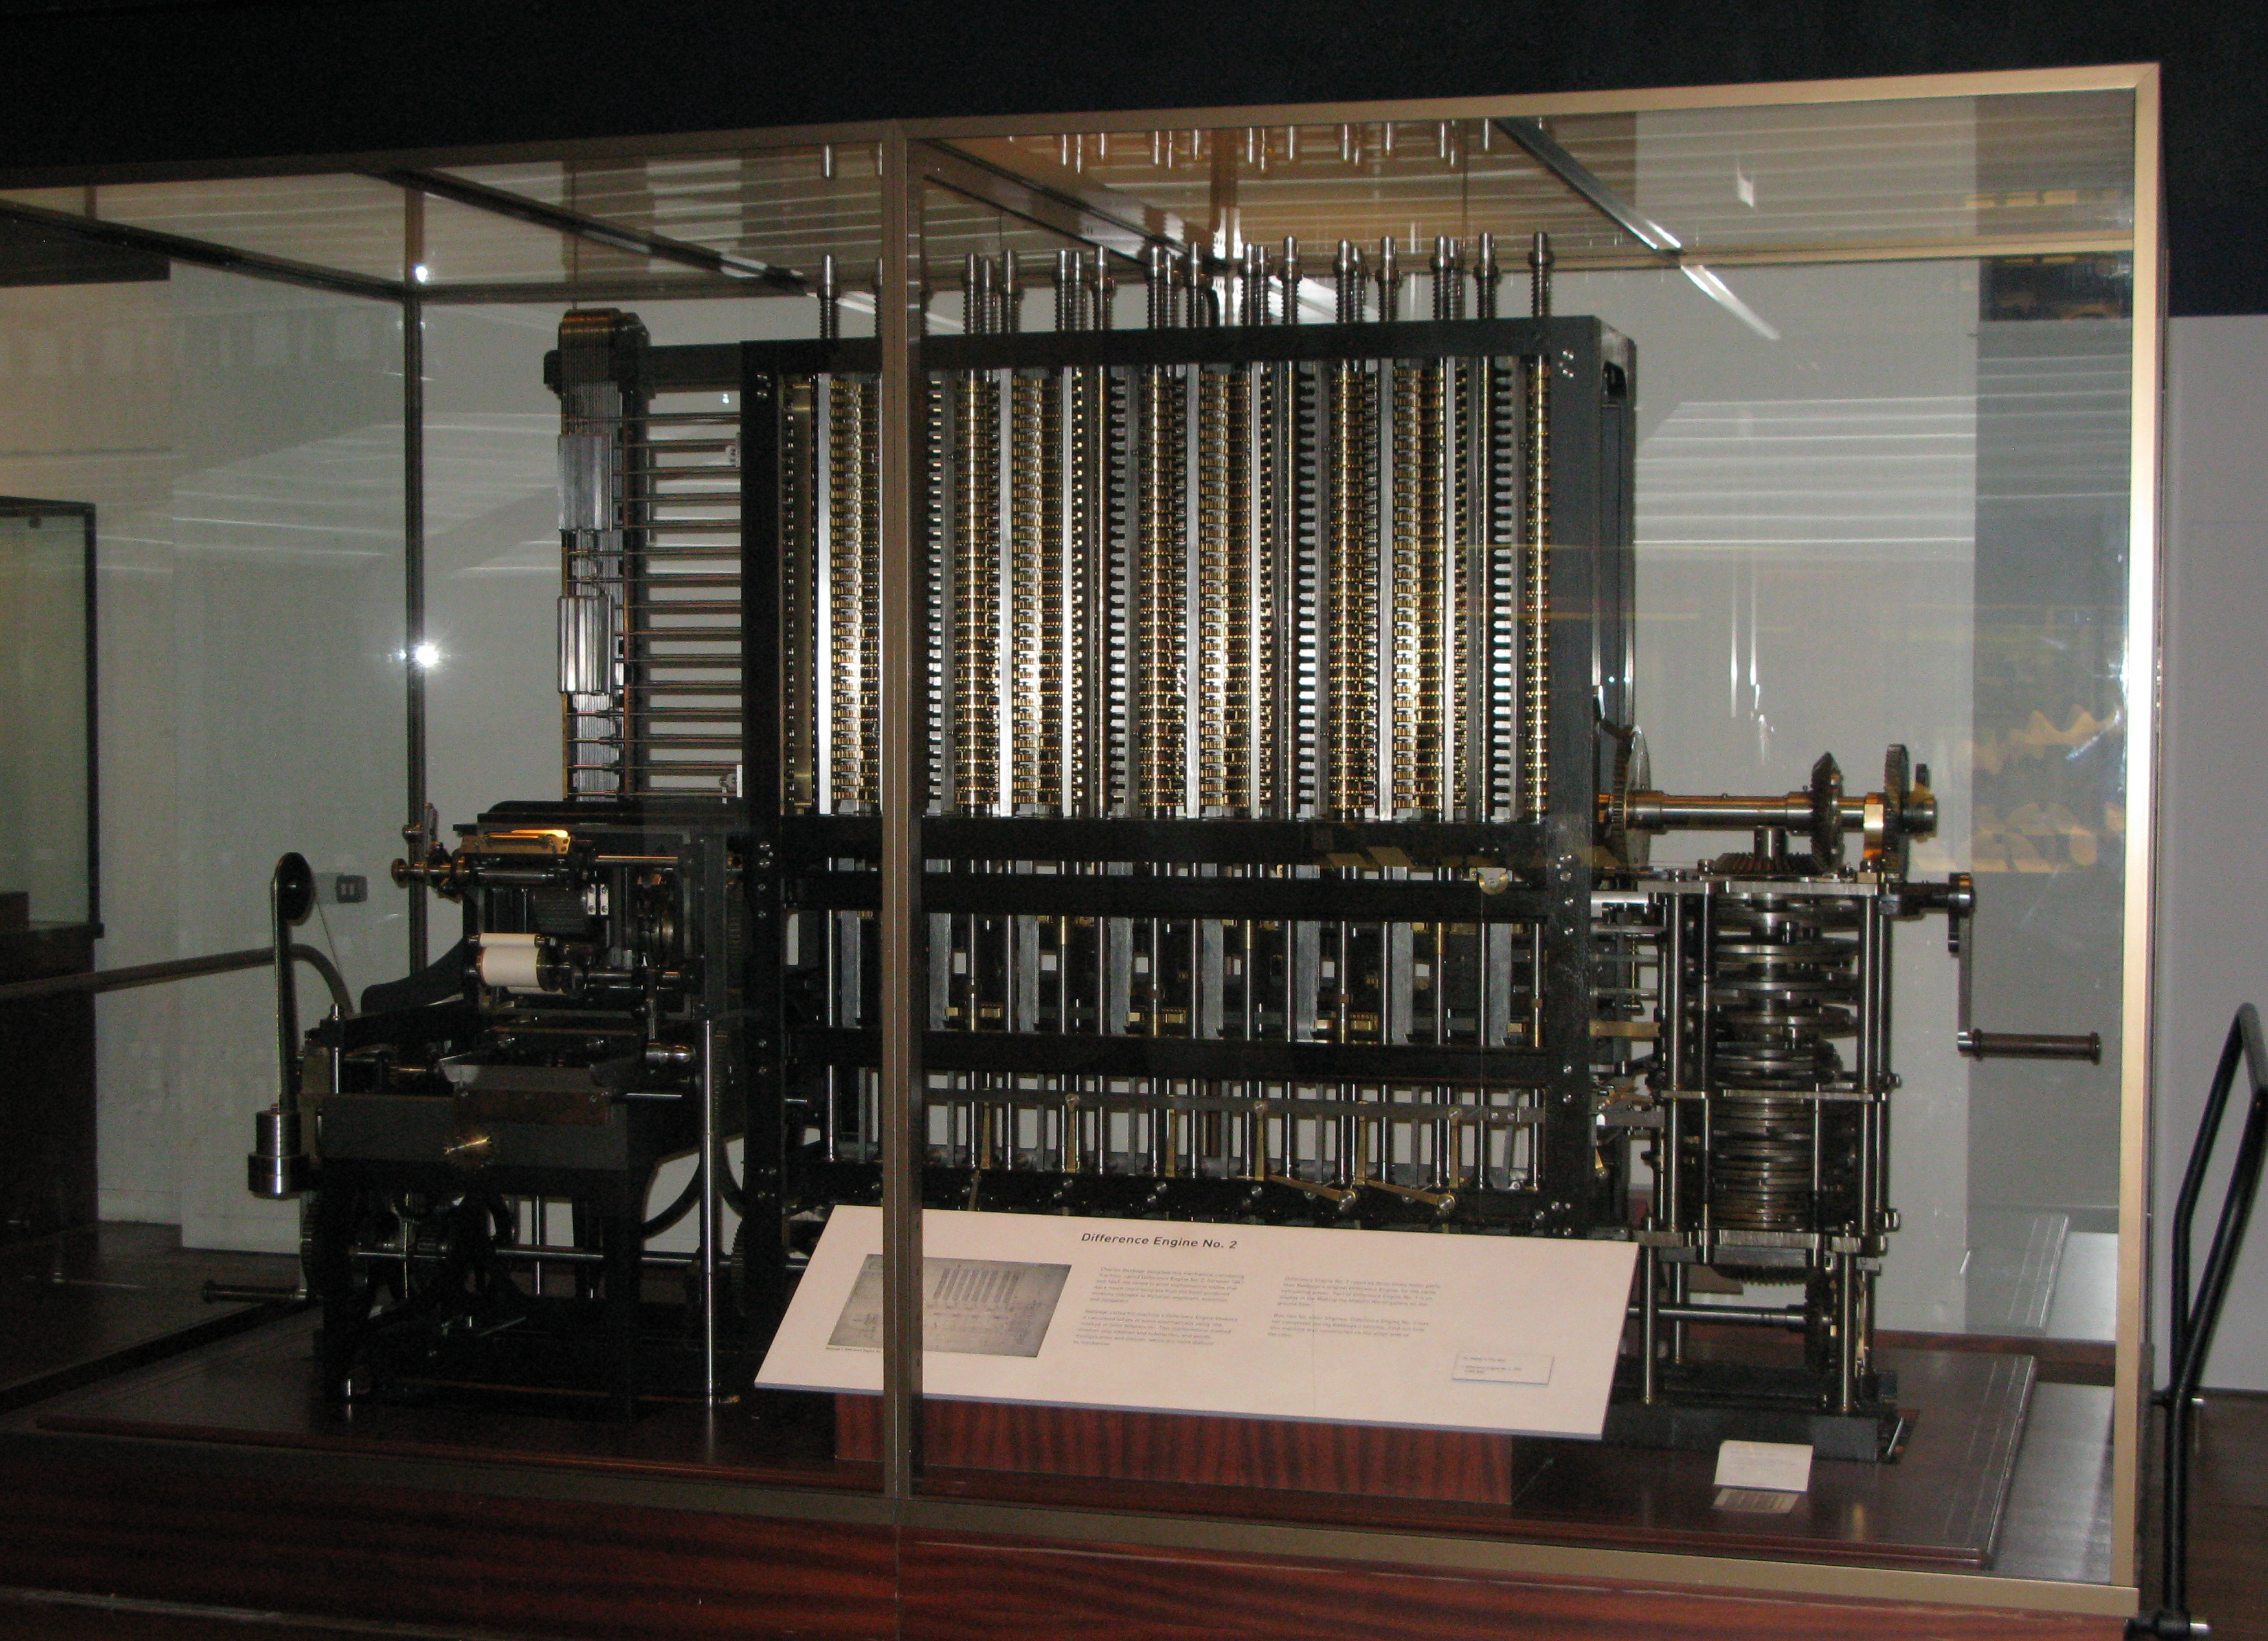
\includegraphics[width=\columnwidth]{../../../img/diferencial_2.jpg}
\caption{\alert{Máquina Diferencial} de Charles Babbage}
\end{figure}
}

\only<7>{
\begin{figure}[htbp]
\centering
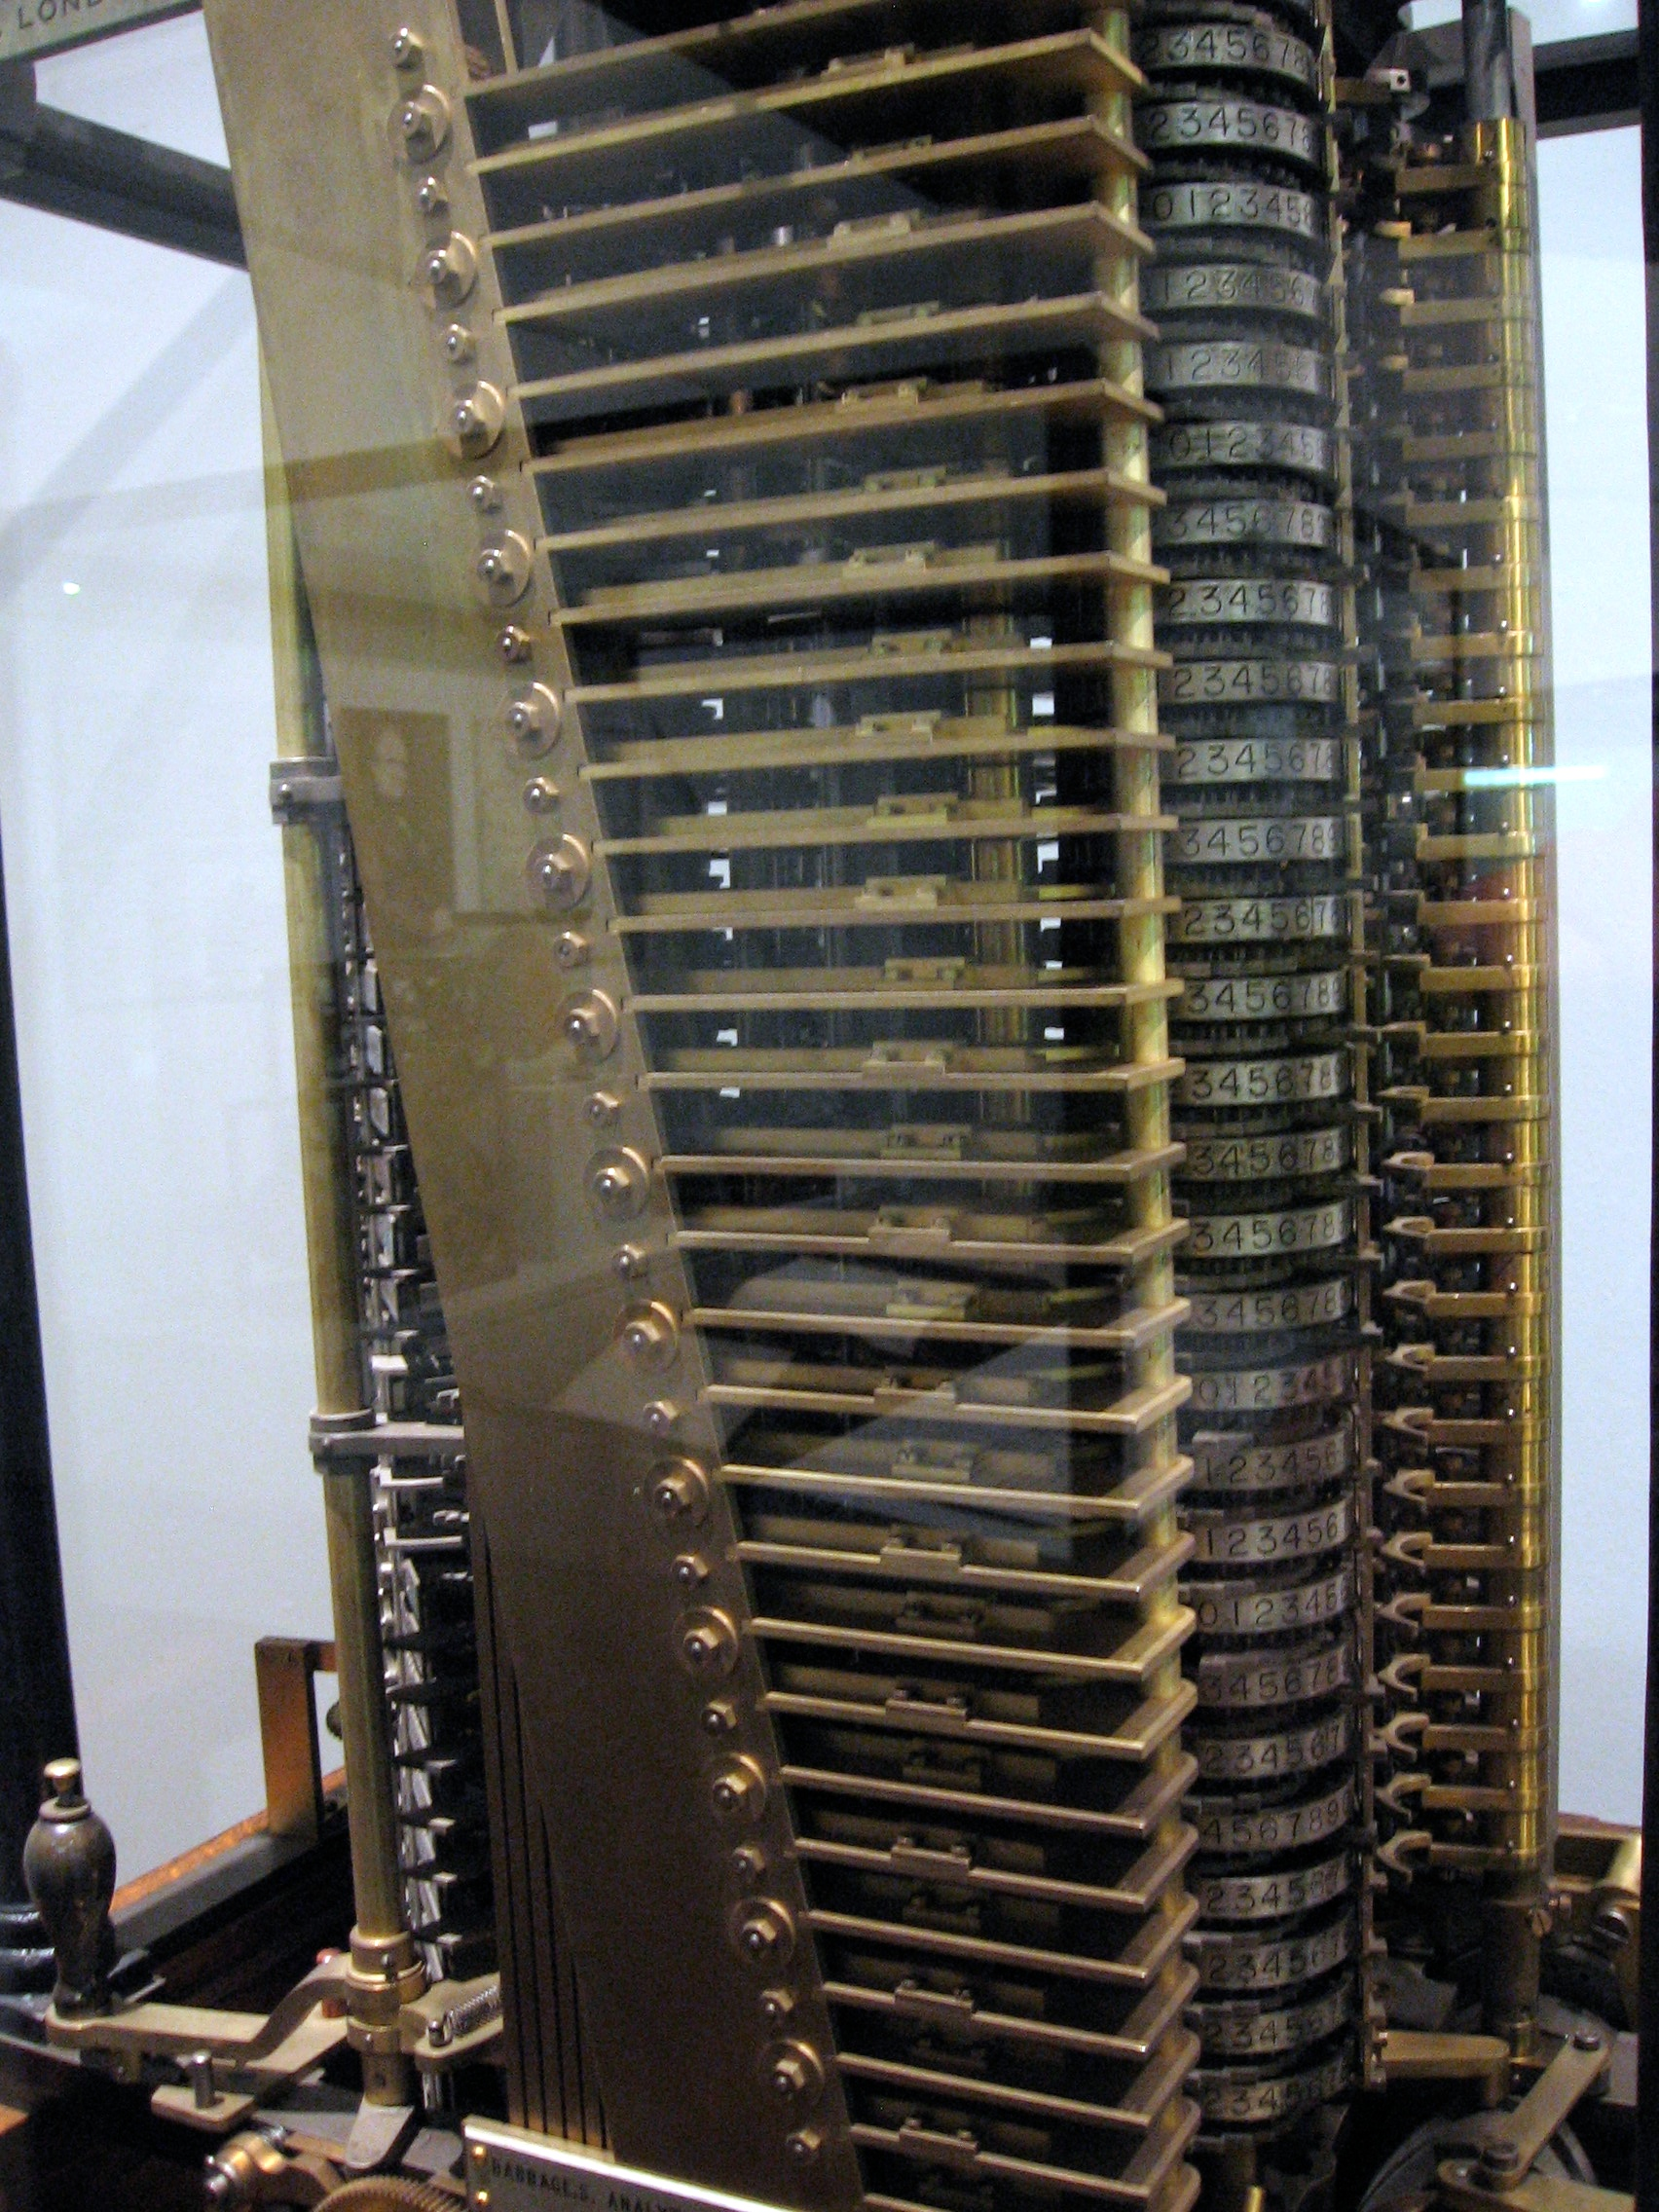
\includegraphics[width=.62\columnwidth]{../../../img/analitica.jpg}
\caption{\alert{Máquina Analítica} de Charles Babbage}
\end{figure}
}

\only<8>{
\begin{figure}[htbp]
\centering
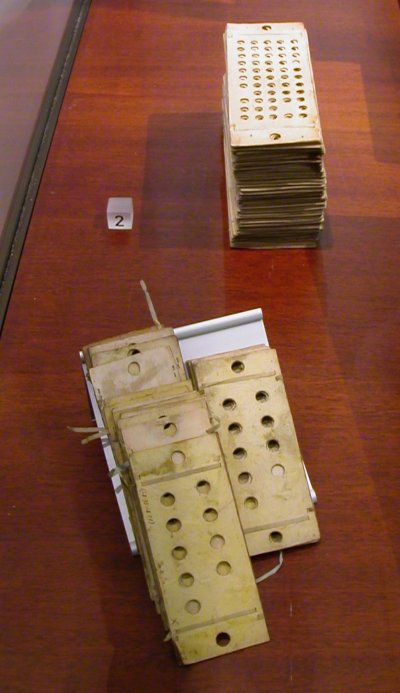
\includegraphics[width=.48\columnwidth]{../../../img/analitica_programas.jpg}
\caption{``\alert{Programas}'' para a Máquina Analítica}
\end{figure}
}

\only<9>{
\begin{figure}[htbp]
\centering
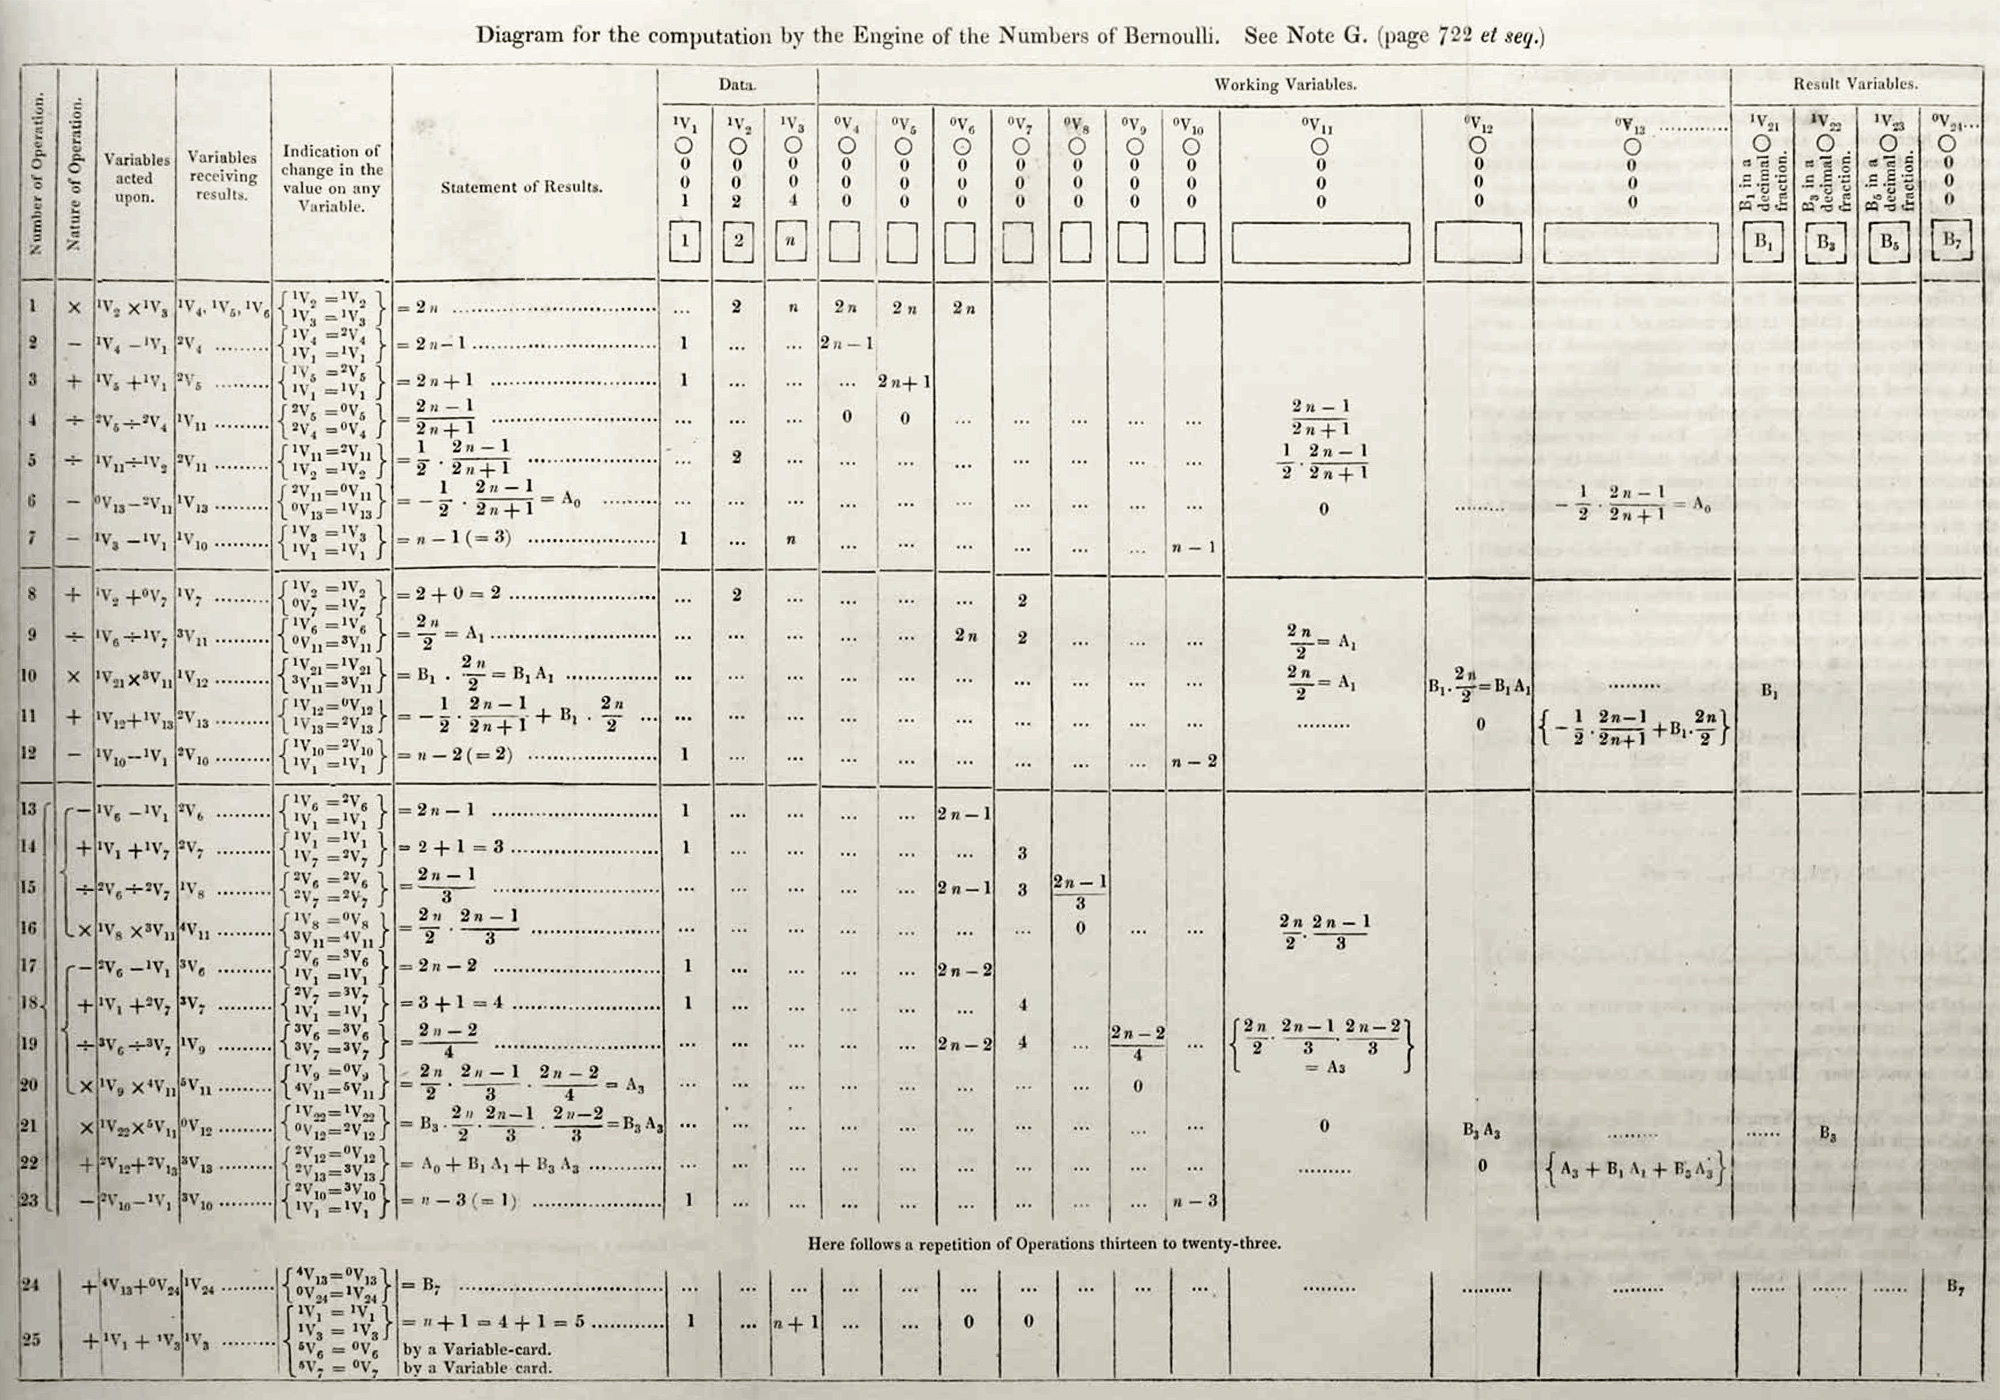
\includegraphics[width=\columnwidth]{../../../img/ada_primeiro_programa_publicado.jpg}
\caption{\alert{Primeiro programa}, por Ada Lovelace}
\end{figure}
}

\only<10>{
\begin{figure}[htbp]
\centering
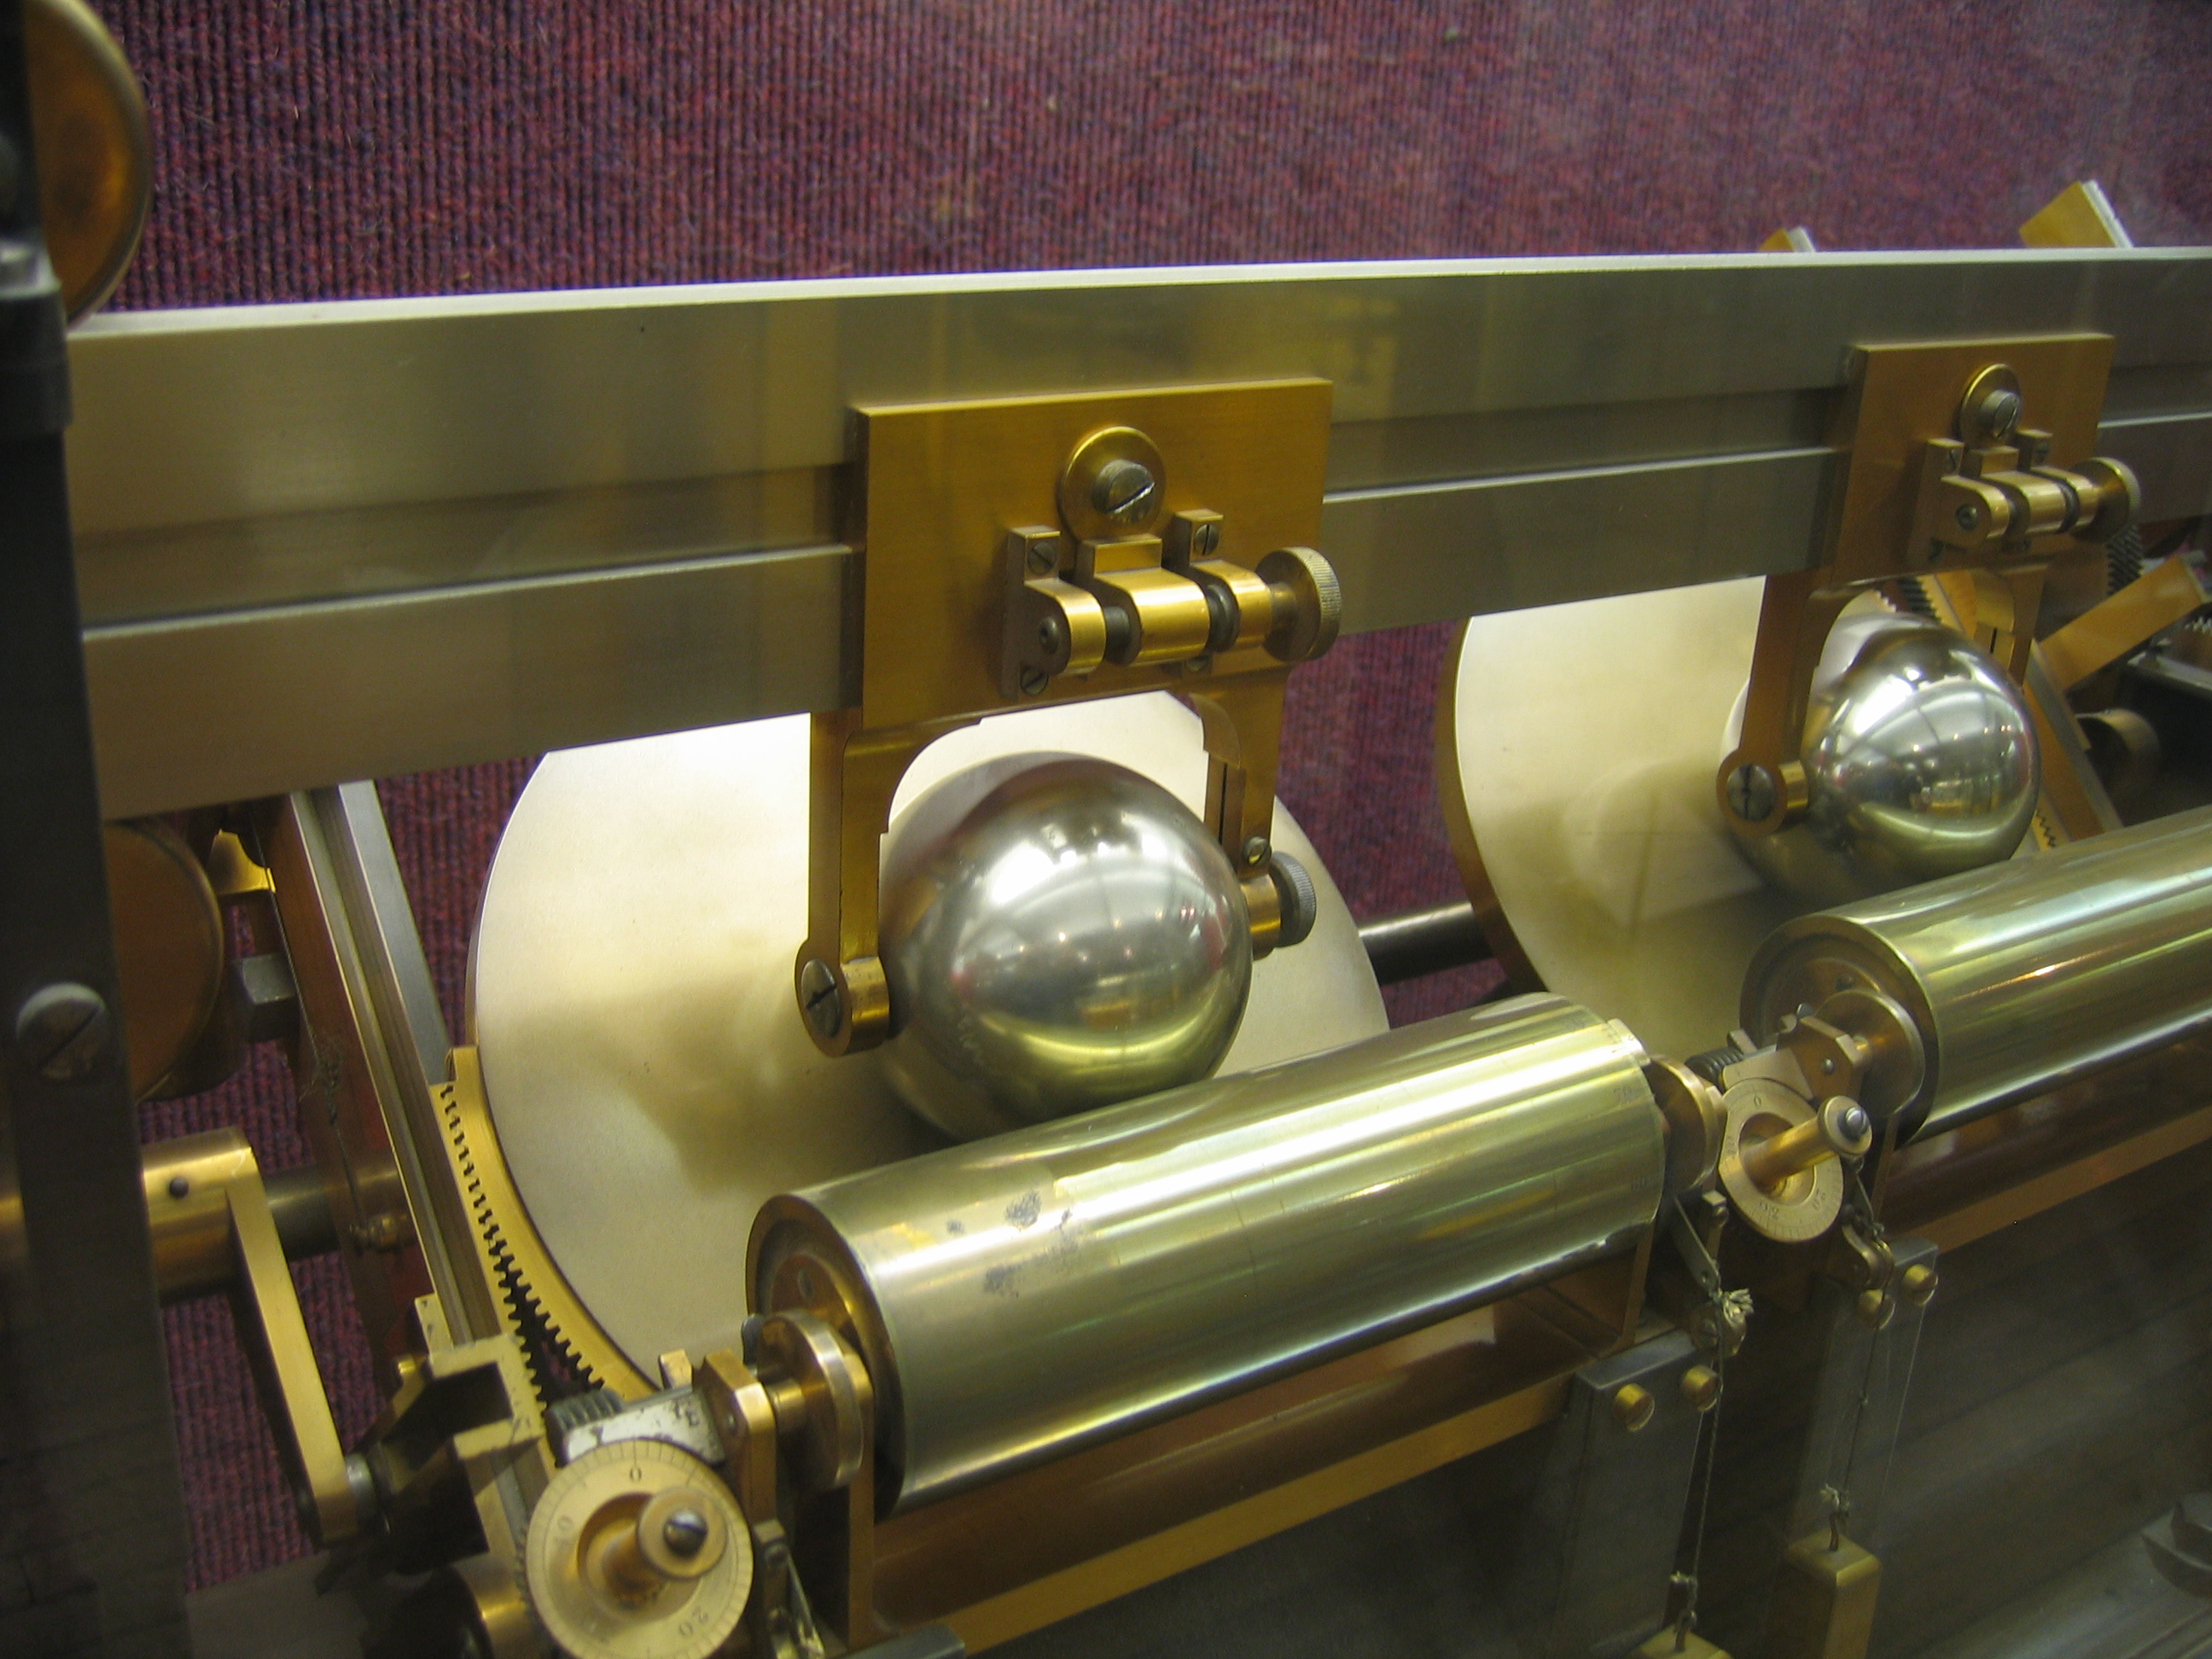
\includegraphics[width=\columnwidth]{../../../img/analisador_diferencial.jpg}
\caption{Analisador Diferencial para \alert{predição de marés}}
\end{figure}
}
\end{column}
\end{columns}
\end{frame}

\begin{frame}[label={sec:org914c0dd}]{Computação no Século 20}
\begin{columns}
\begin{column}{0.5\columnwidth}
\begin{block}{Linha do Tempo}
\begin{itemize}
\item \alert{Tubos de Vácuo}: 1904
\item \visible<2->{Máquina de \alert{Turing}: 1936}
\item \visible<3->{Arquitetura de \alert{Von Neumann}: 1945}
\item \visible<4->{\alert{ENIAC}: 1945}
\item \visible<5->{\alert{Transístor}: 1947}
\item \visible<6->{\alert{Fotolitografia}: 1958}
\item \visible<7->{\alert{Circuito Integrado}: 1958}
\item \visible<8->{\alert{Microprocessador}: 1971}
\item \visible<10->{\alert{Supercomputador}: 1976}
\item \visible<12->{\alert{Laptops}: anos 1990}
\item \visible<13->{\alert{Smartphones}: anos 2000}
\end{itemize}
\end{block}
\end{column}

\begin{column}{0.5\columnwidth}
\only<1>{
\begin{figure}[htbp]
\centering
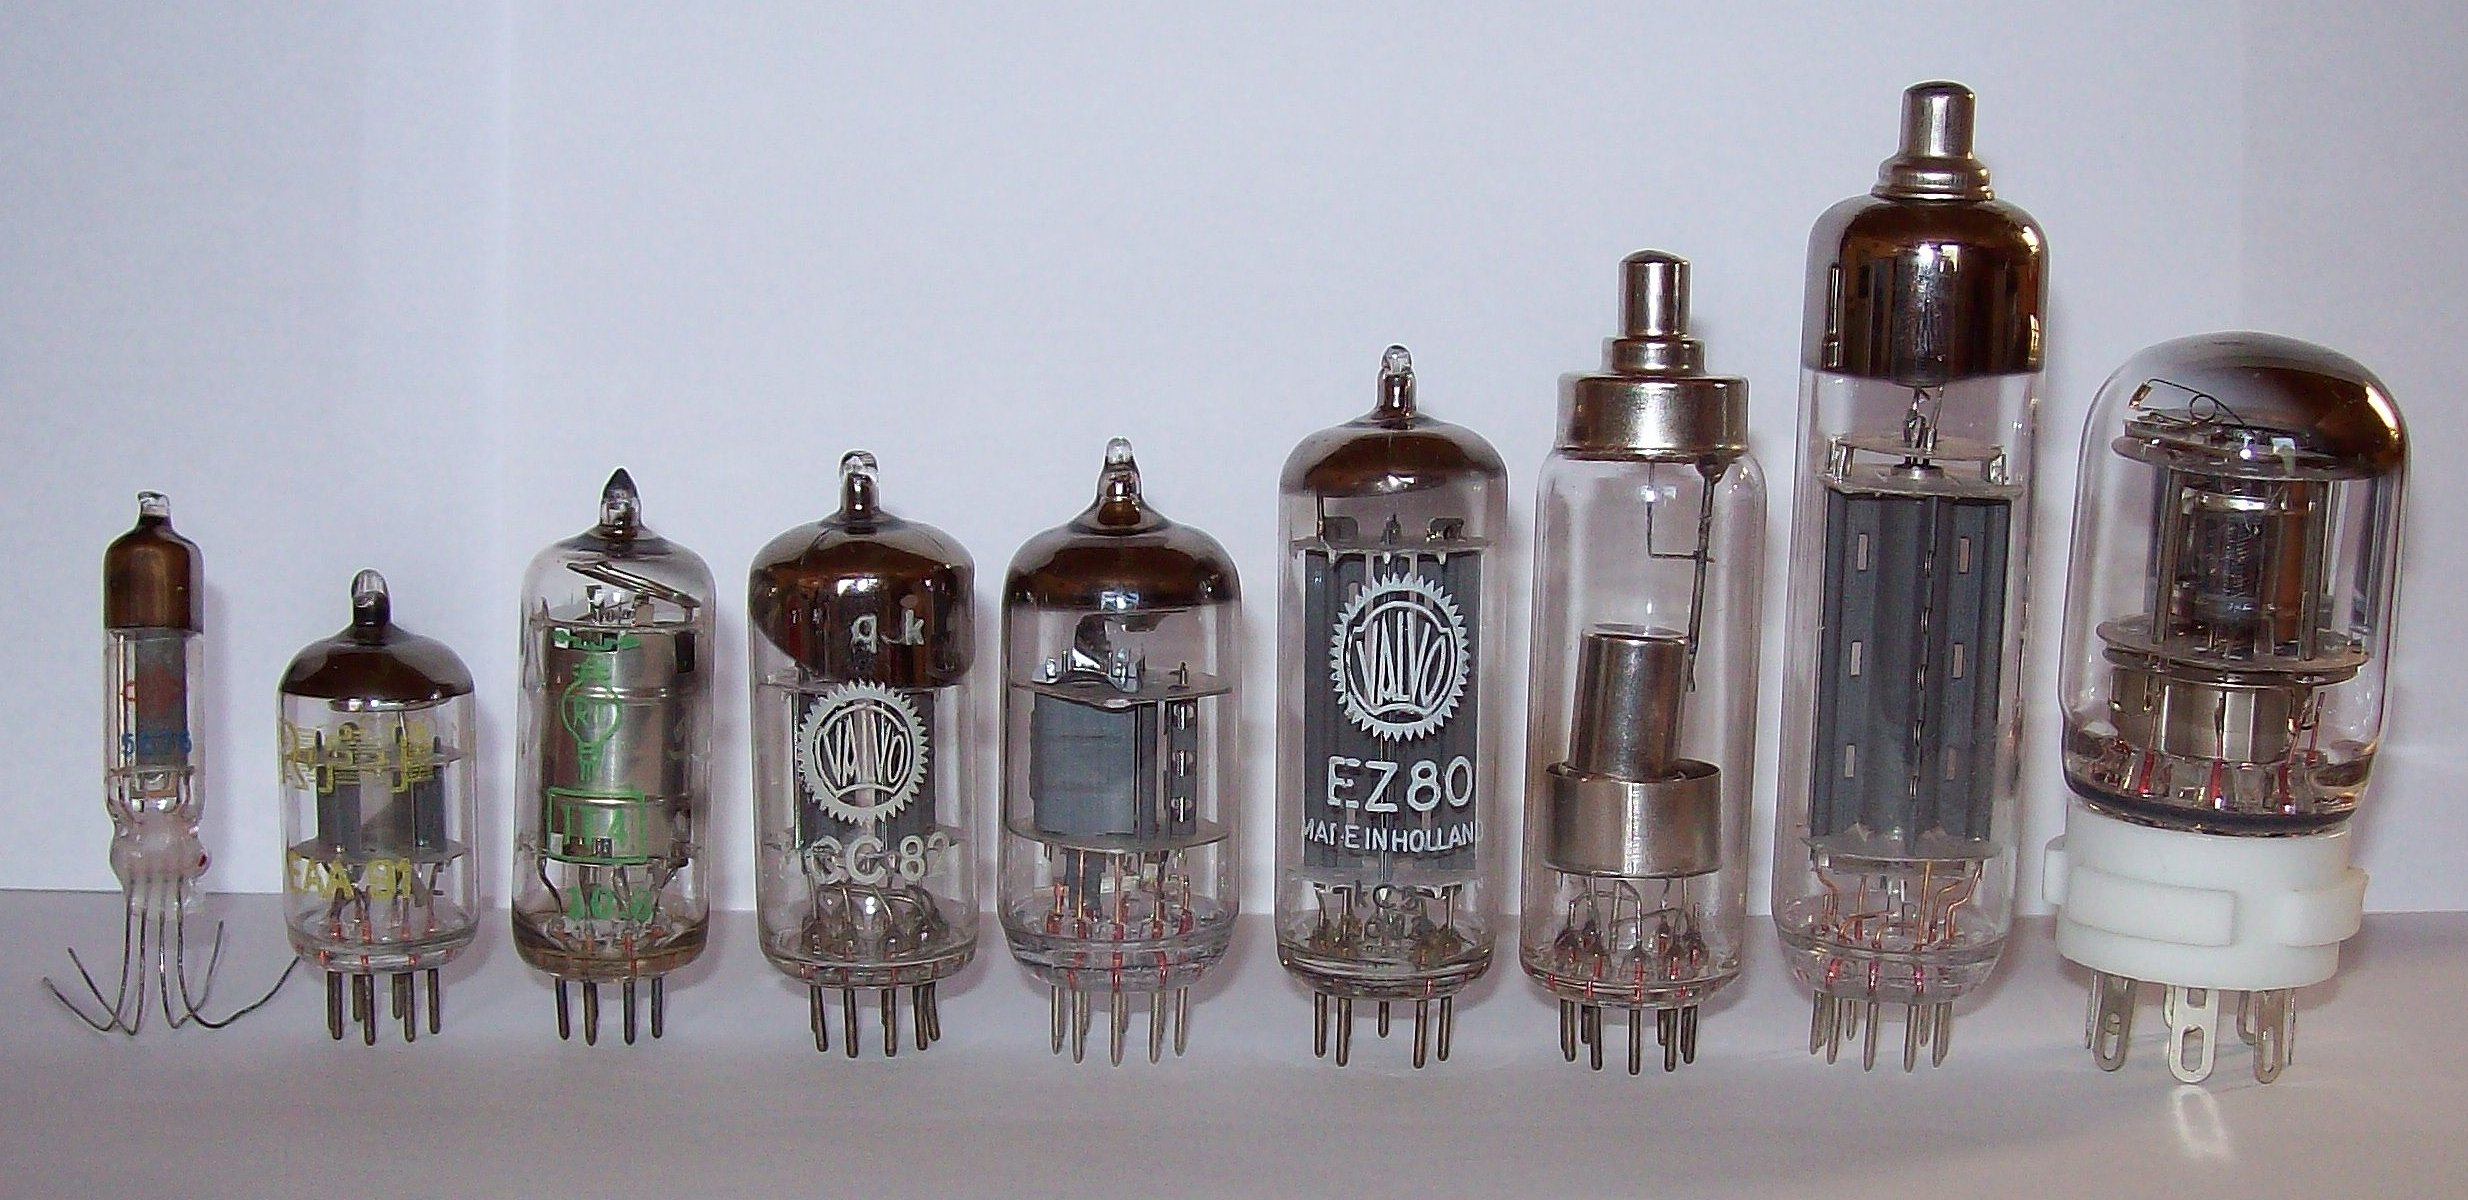
\includegraphics[width=\columnwidth]{../../../img/tubos_vacuo.jpg}
\caption{Tubos de Vácuo, ou \alert{Válvulas}}
\end{figure}
}

\only<2>{
\begin{figure}[htbp]
\centering
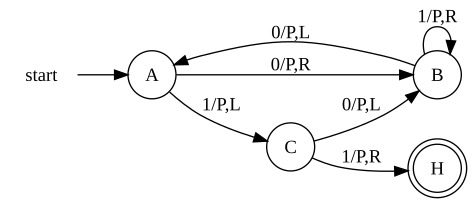
\includegraphics[width=1.0\columnwidth]{../../../img/automato.jpg}
\caption{Representação de uma Máquina de \alert{Turing}}
\end{figure}
}

\only<3>{
\begin{figure}[htbp]
\centering
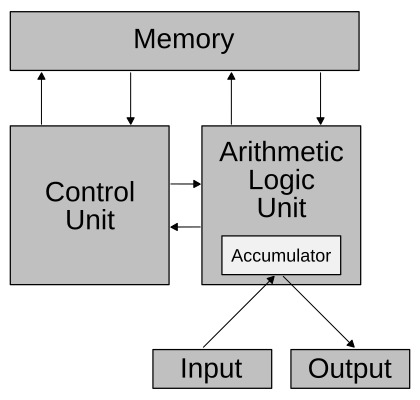
\includegraphics[width=.8\columnwidth]{../../../img/arquitetura_neumann.jpg}
\caption{Arquitetura de \alert{Von Neumann}}
\end{figure}
}

\only<4>{
\begin{figure}[htbp]
\centering
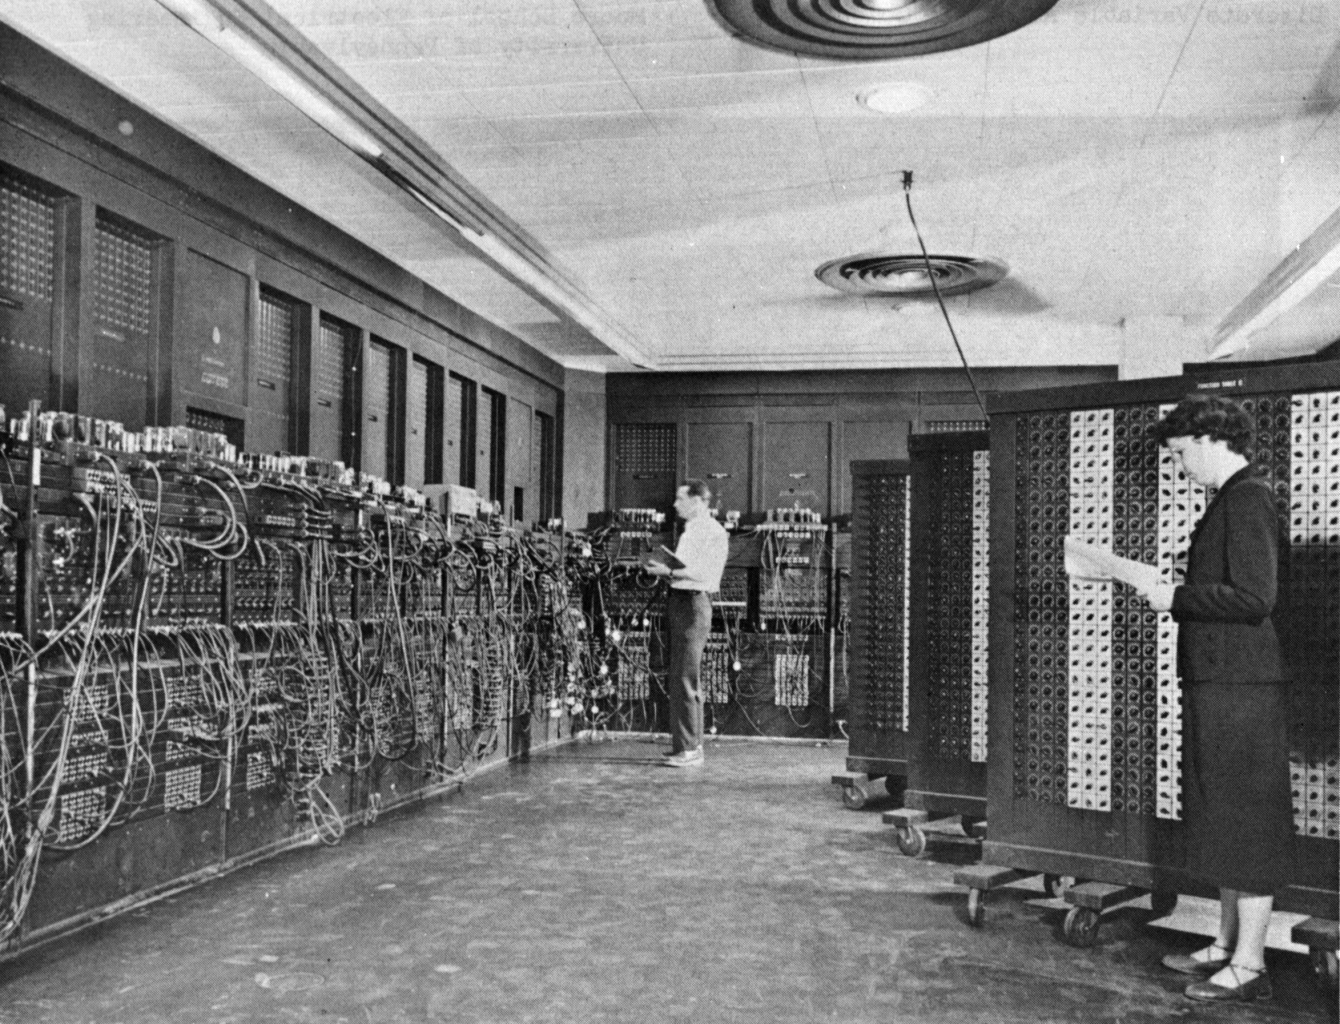
\includegraphics[width=1.0\columnwidth]{../../../img/eniac.jpg}
\caption{Sala do \alert{ENIAC}}
\end{figure}
}

\only<5>{
\begin{figure}[htbp]
\centering
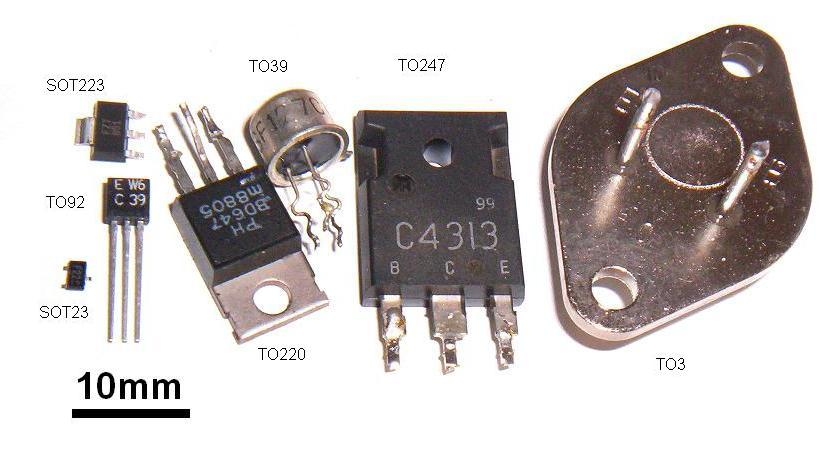
\includegraphics[width=\columnwidth]{../../../img/transistores.jpg}
\caption{Alguns \alert{transistores}}
\end{figure}
}

\only<6>{
\begin{figure}[htbp]
\centering
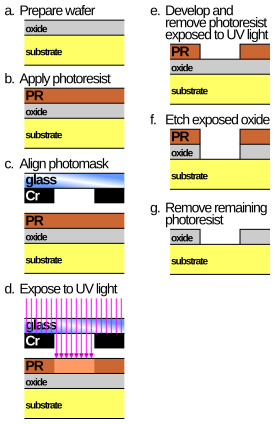
\includegraphics[width=.55\columnwidth]{../../../img/fotolitografia.jpg}
\caption{Processo da \alert{Fotolitografia}}
\end{figure}
}

\only<7>{
\begin{figure}[htbp]
\centering
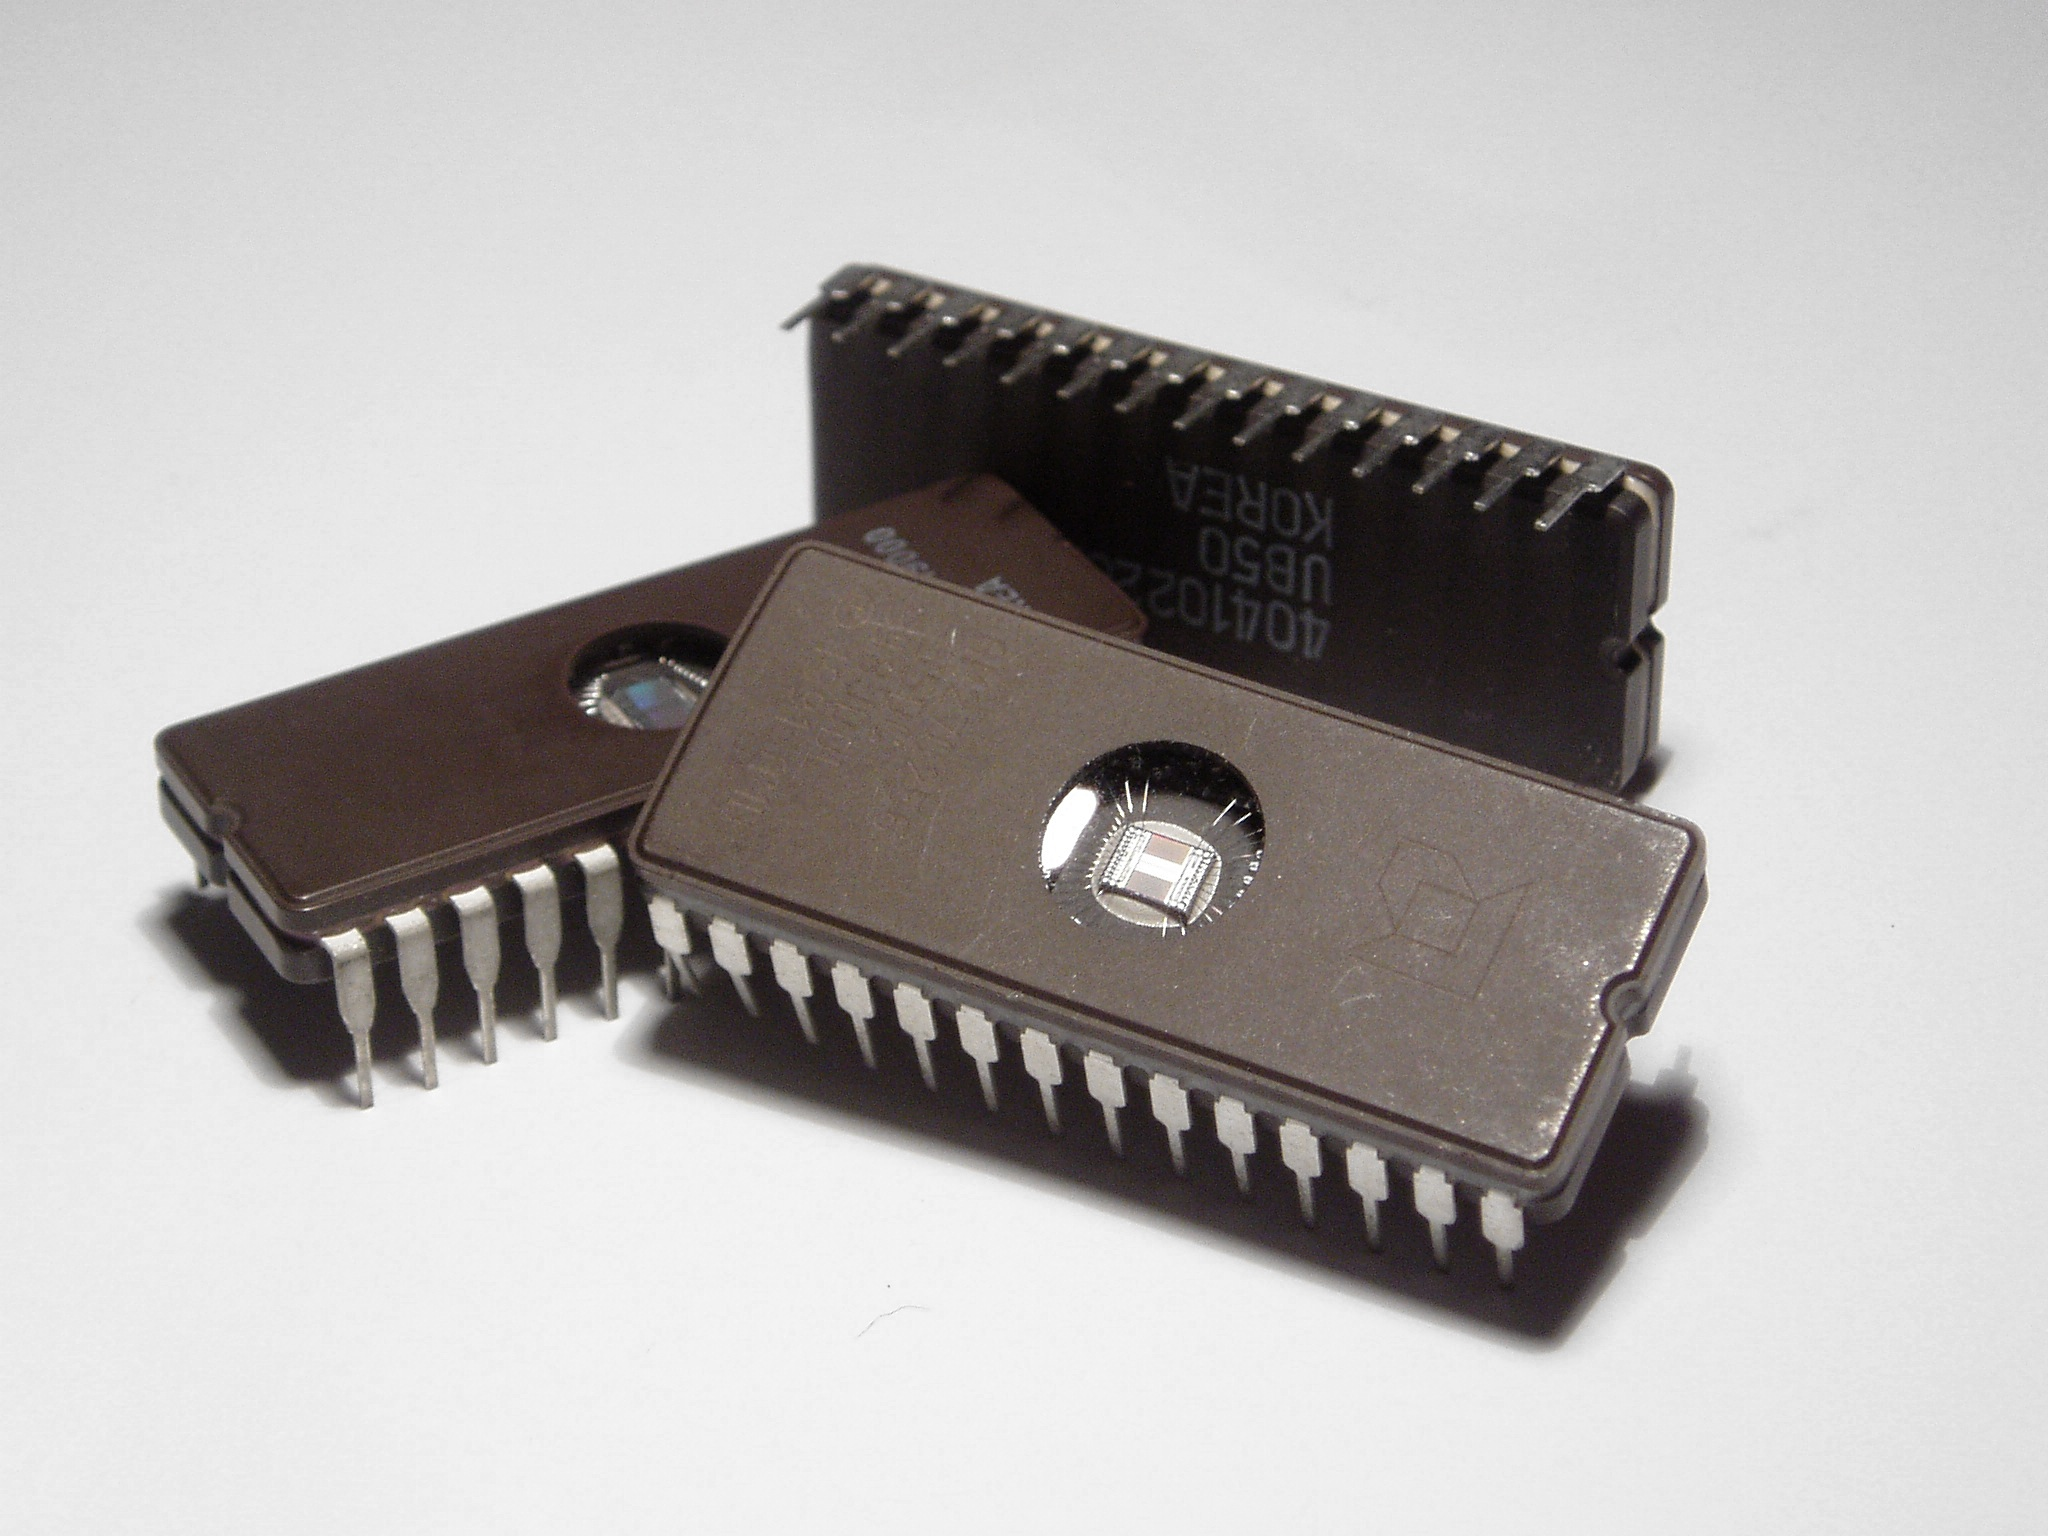
\includegraphics[width=1.0\columnwidth]{../../../img/circuito_integrado.jpg}
\caption{Exemplo de \alert{Circuito Integrado}}
\end{figure}
}

\only<8>{
\begin{figure}[htbp]
\centering
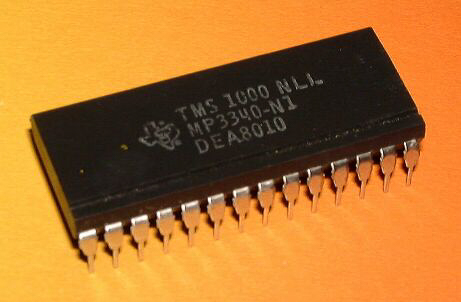
\includegraphics[width=1.0\columnwidth]{../../../img/microprocessador.jpg}
\caption{Exemplo de \alert{Microprocessador}}
\end{figure}
}

\only<9>{
\begin{figure}[htbp]
\centering
\includegraphics[width=.55\columnwidth]{../../../img/eniac_num_chip.jpg}
\caption{\alert{ENIAC} num \alert{único chip}}
\end{figure}
}

\only<10>{
\begin{figure}[htbp]
\centering
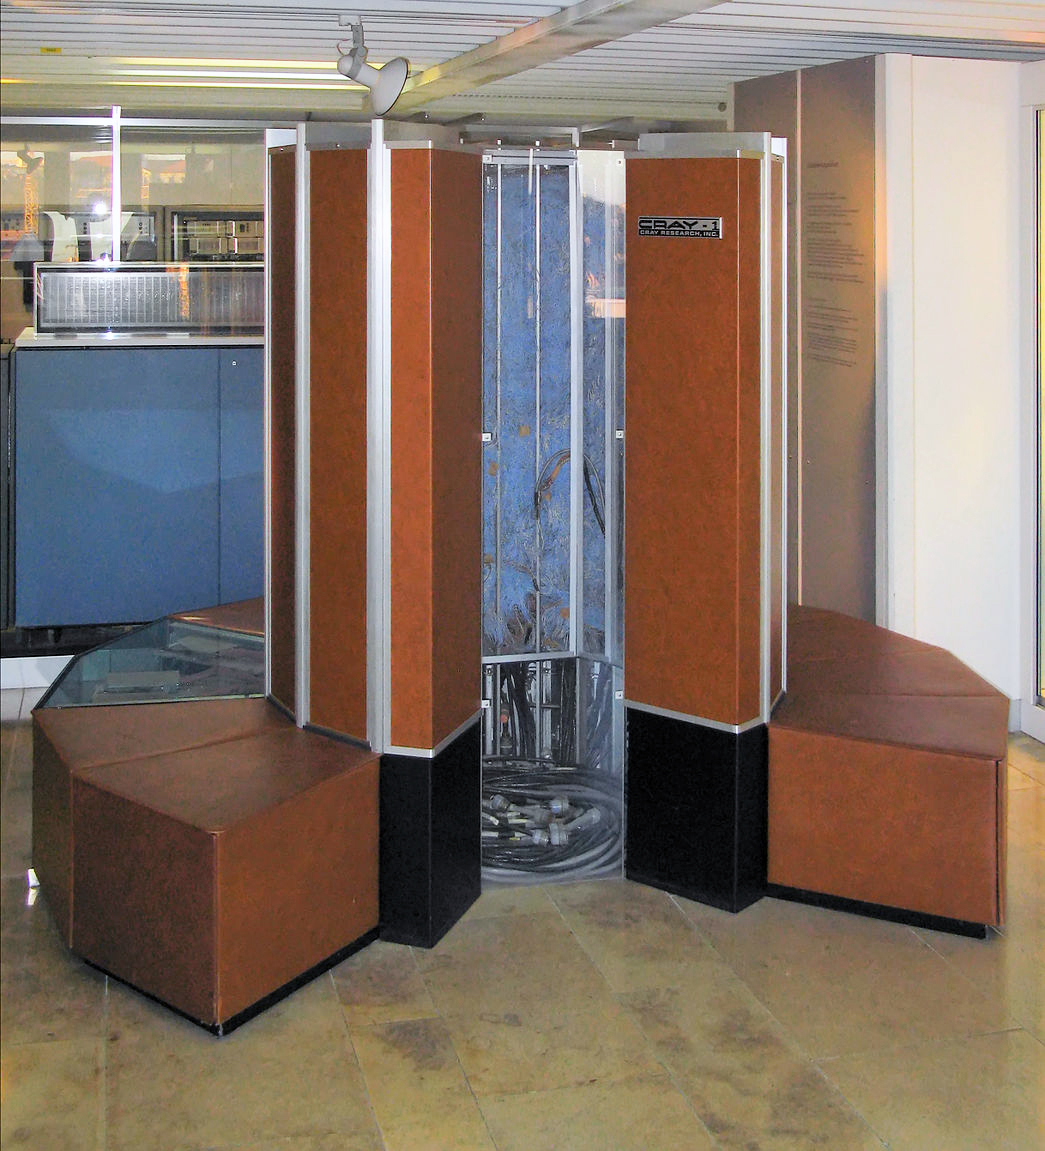
\includegraphics[width=.8\columnwidth]{../../../img/cray1.jpg}
\caption{Supercomputador \alert{Cray-1}, década de 1970}
\end{figure}
}

\only<11>{
\begin{figure}[htbp]
\centering
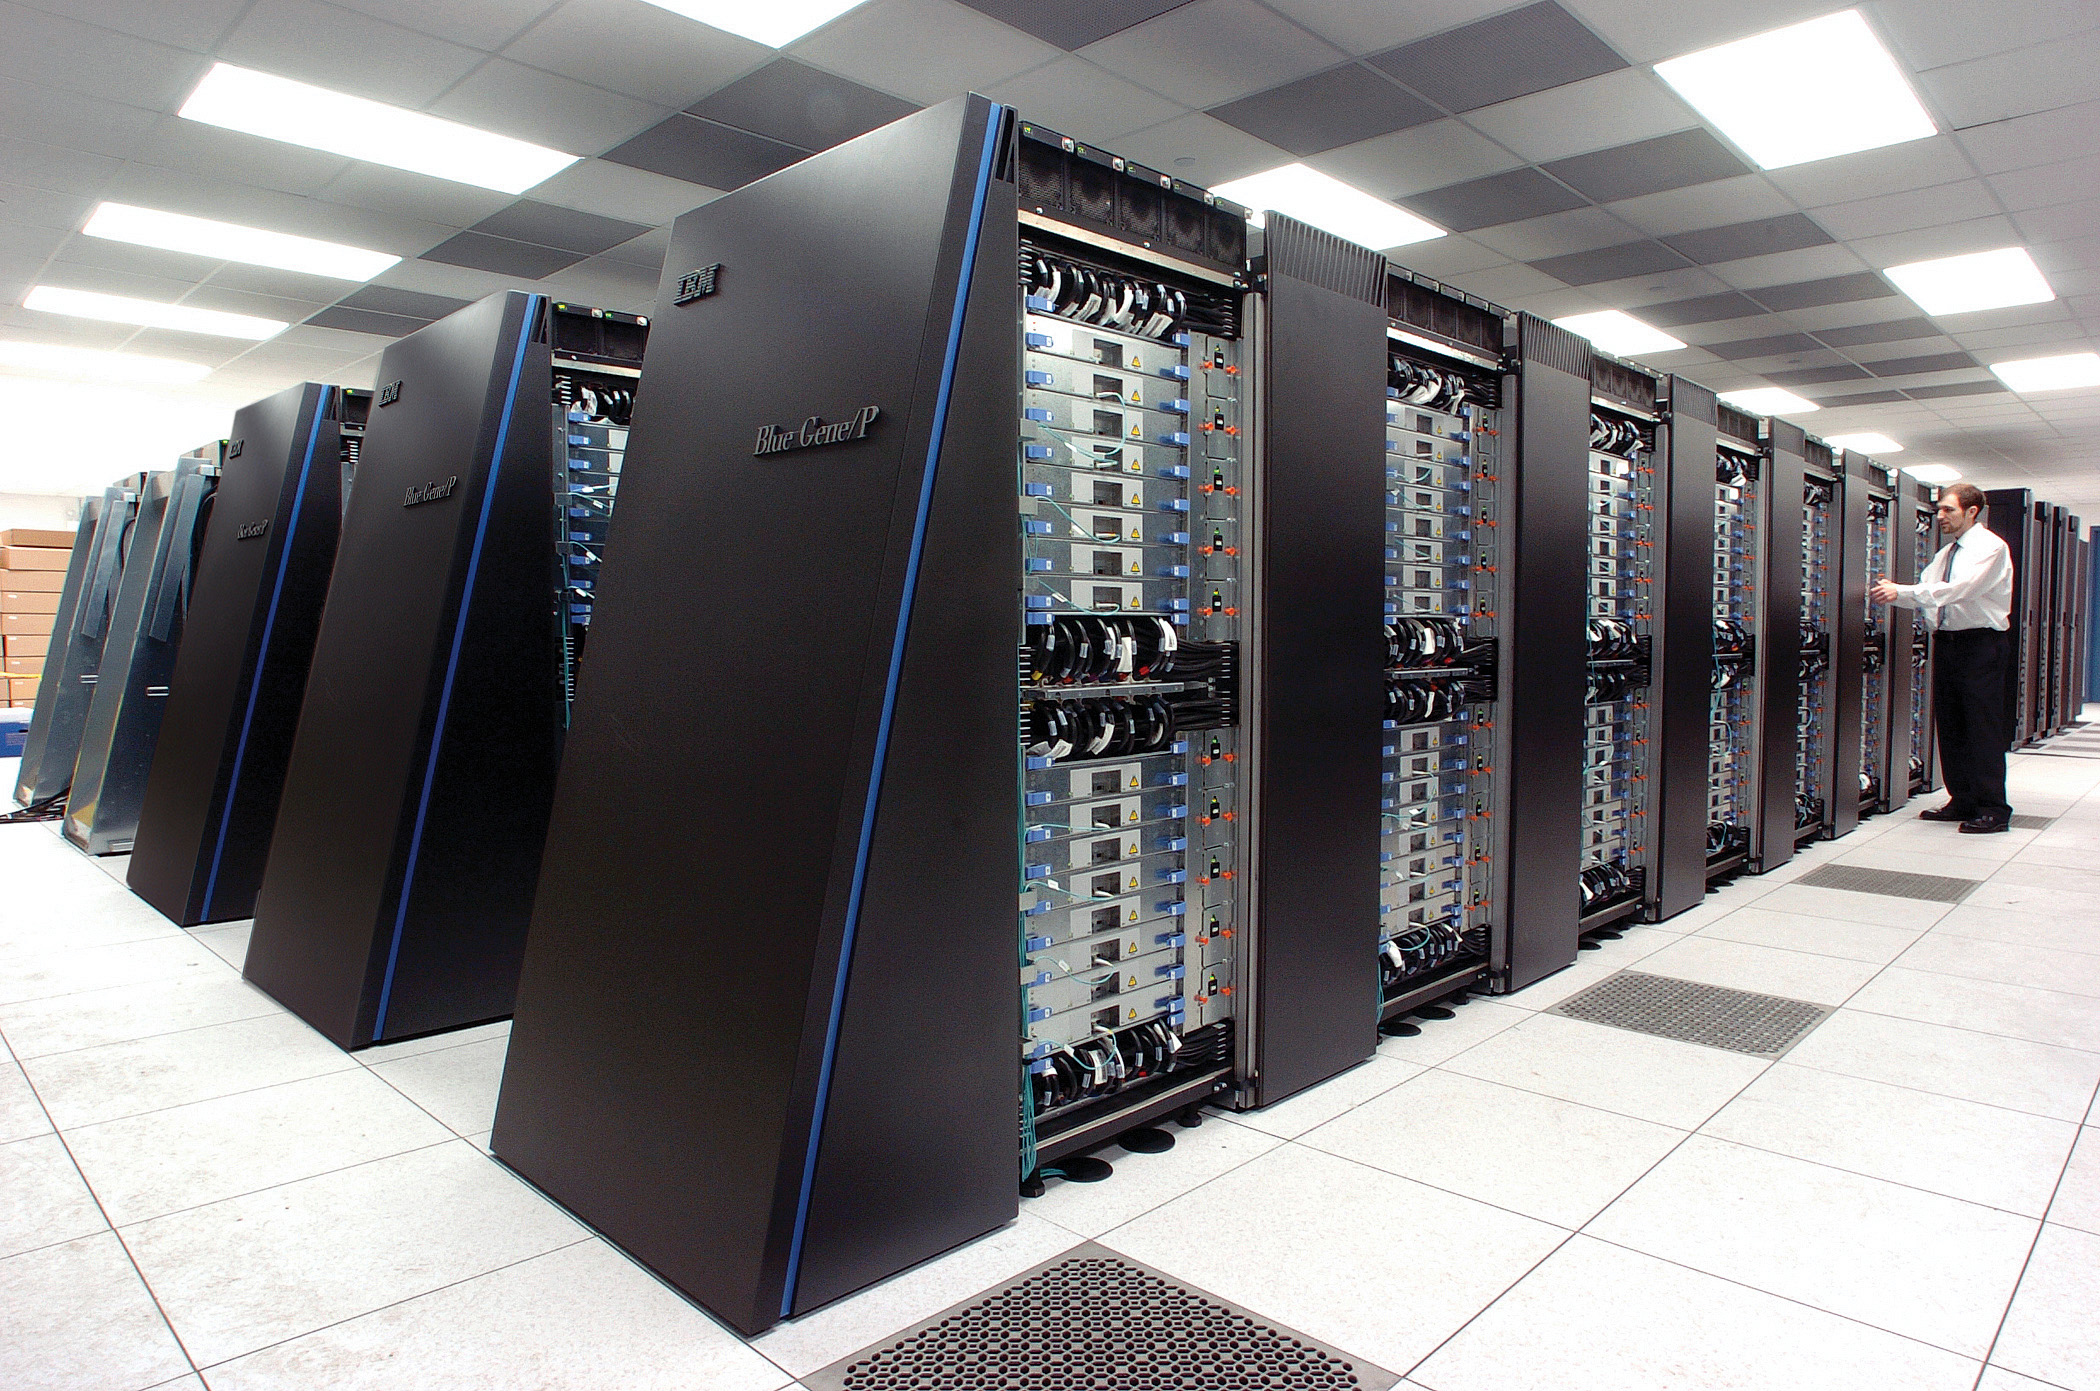
\includegraphics[width=\columnwidth]{../../../img/blue_gene.jpg}
\caption{Supercomputador \alert{Blue Gene P}, 2007}
\end{figure}
}

\only<12>{
\begin{figure}[htbp]
\centering
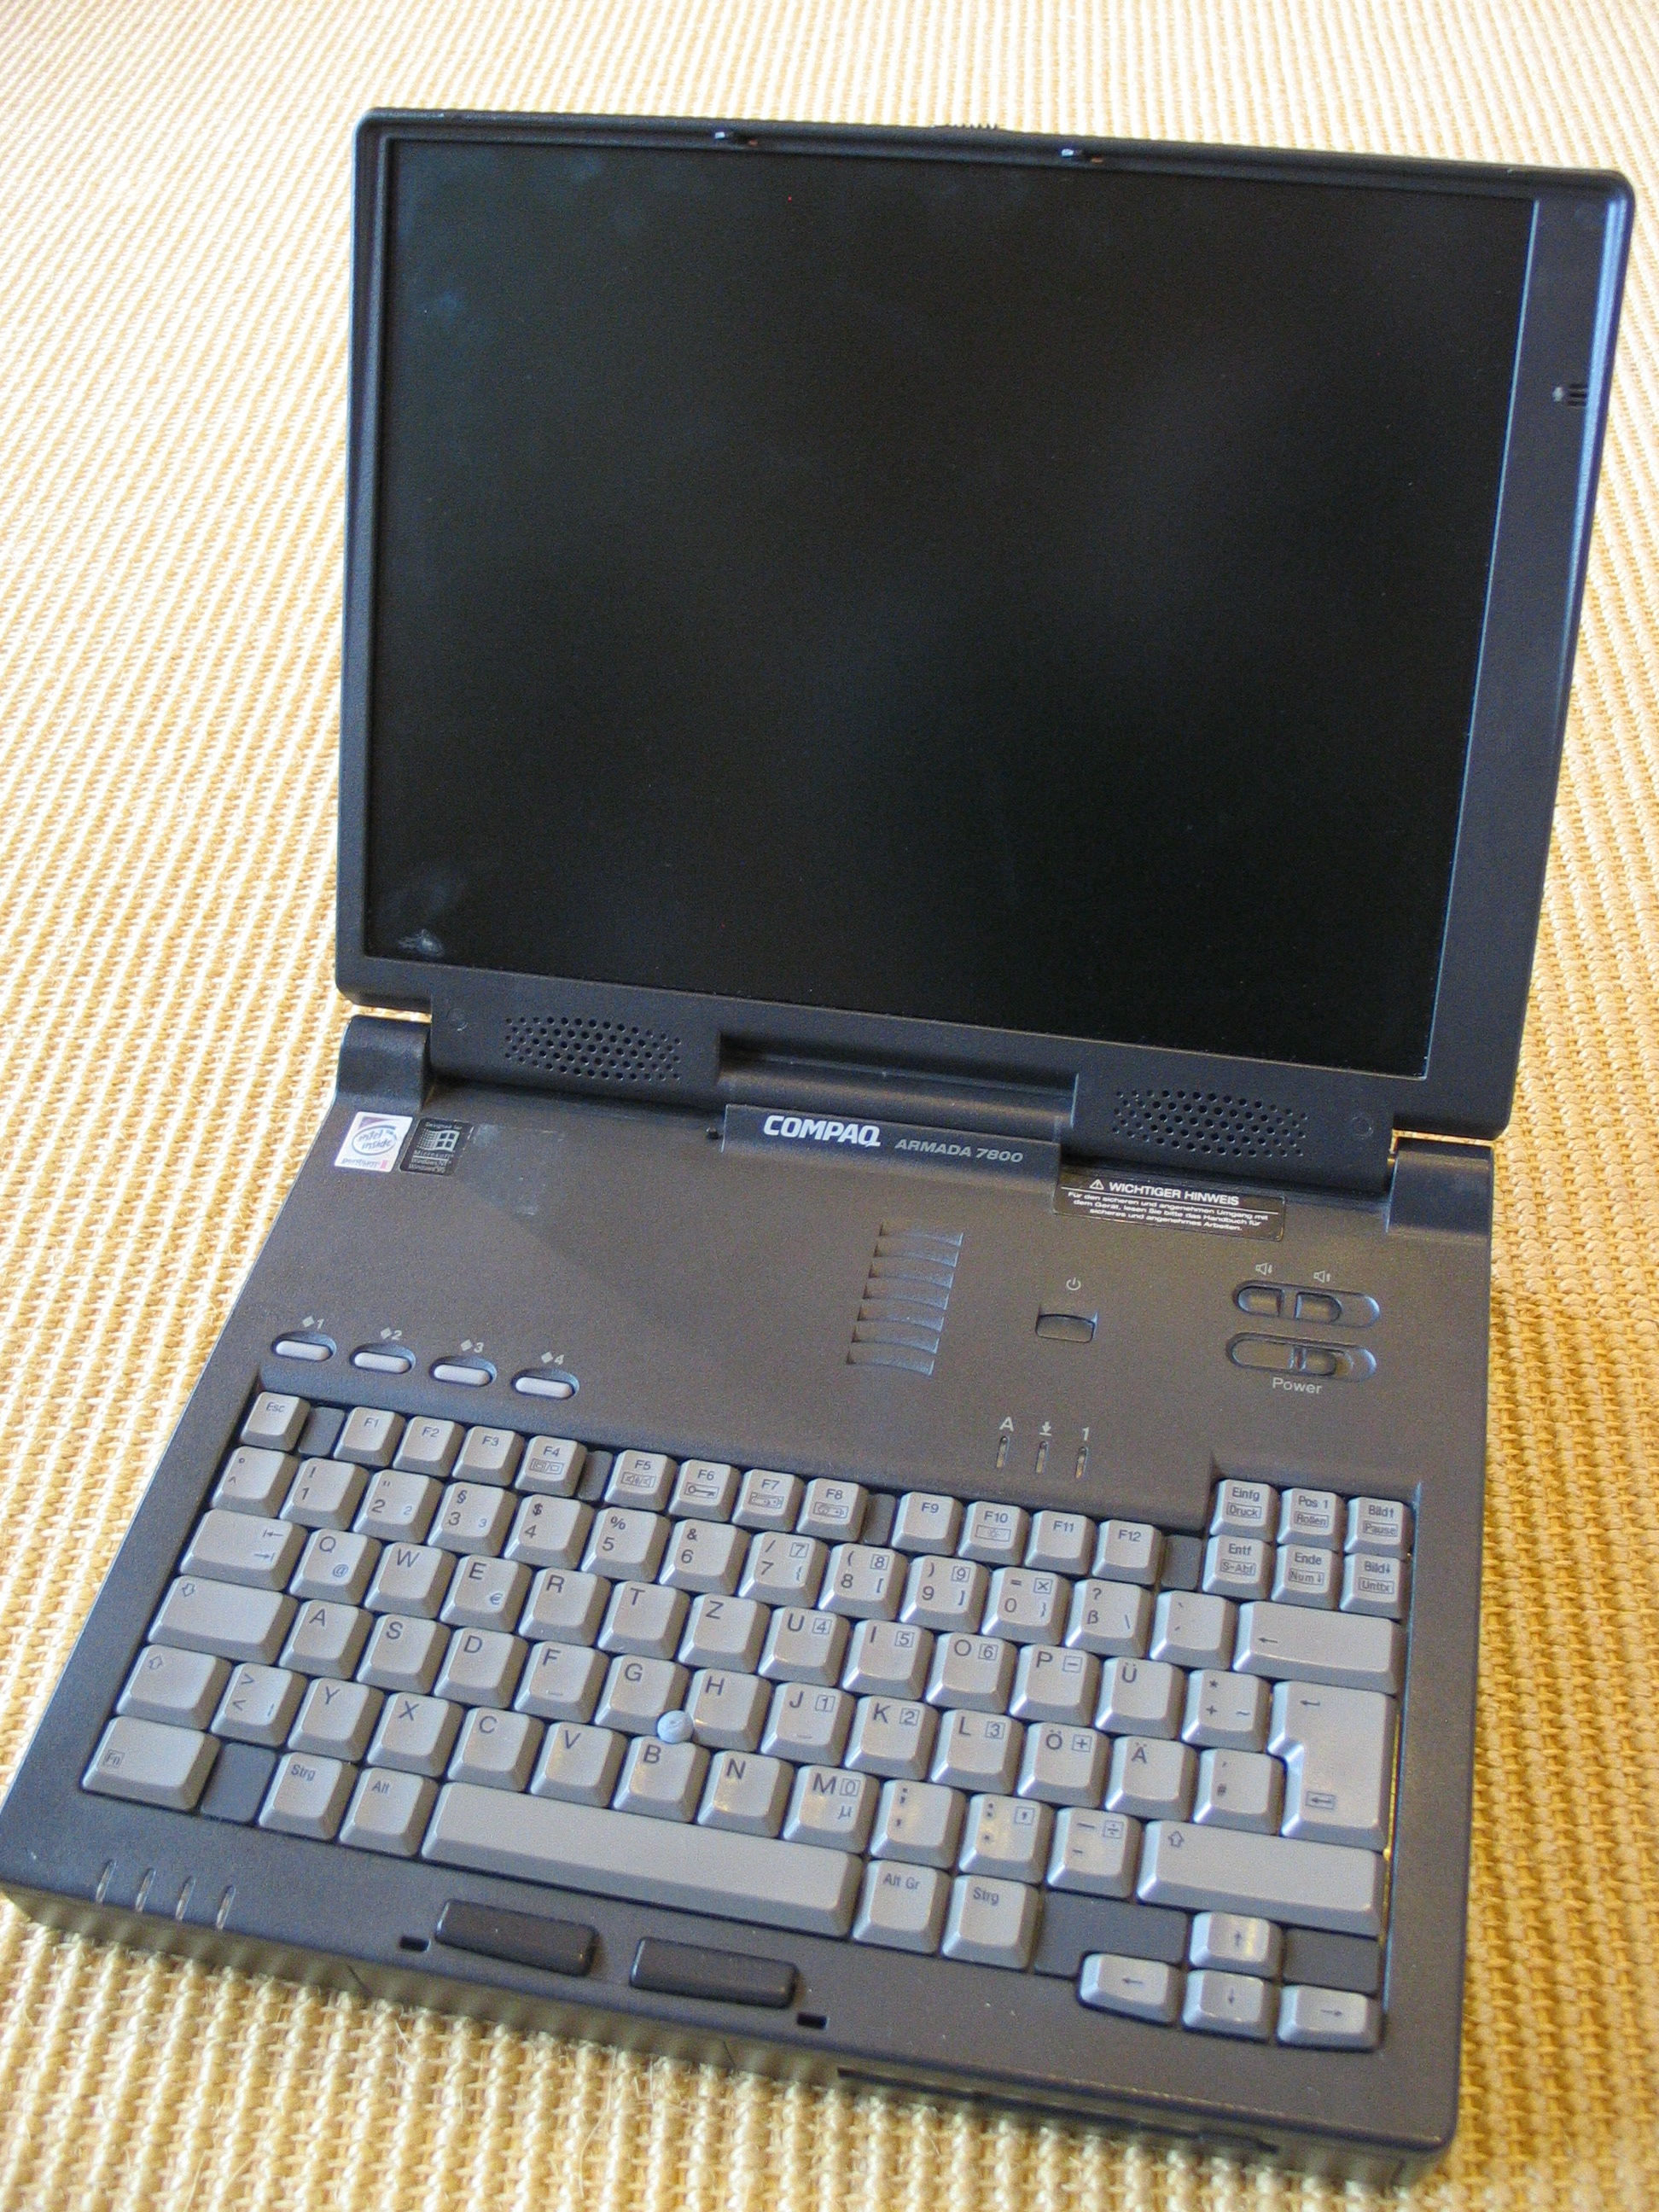
\includegraphics[width=.6\columnwidth]{../../../img/compaq_armada.jpg}
\caption{\alert{Compaq Armada}, década de 1990}
\end{figure}
}

\only<13>{
\begin{figure}[htbp]
\centering

\includegraphics[width=.4\columnwidth]{../../../img/iphone1.jpg}
\caption{Primeiro \alert{iPhone}, década de 2000}
\end{figure}
}
\end{column}
\end{columns}
\end{frame}

\begin{frame}[label={sec:org8666466}]{Linguagens de Programação}
\begin{figure}[htbp]
\centering
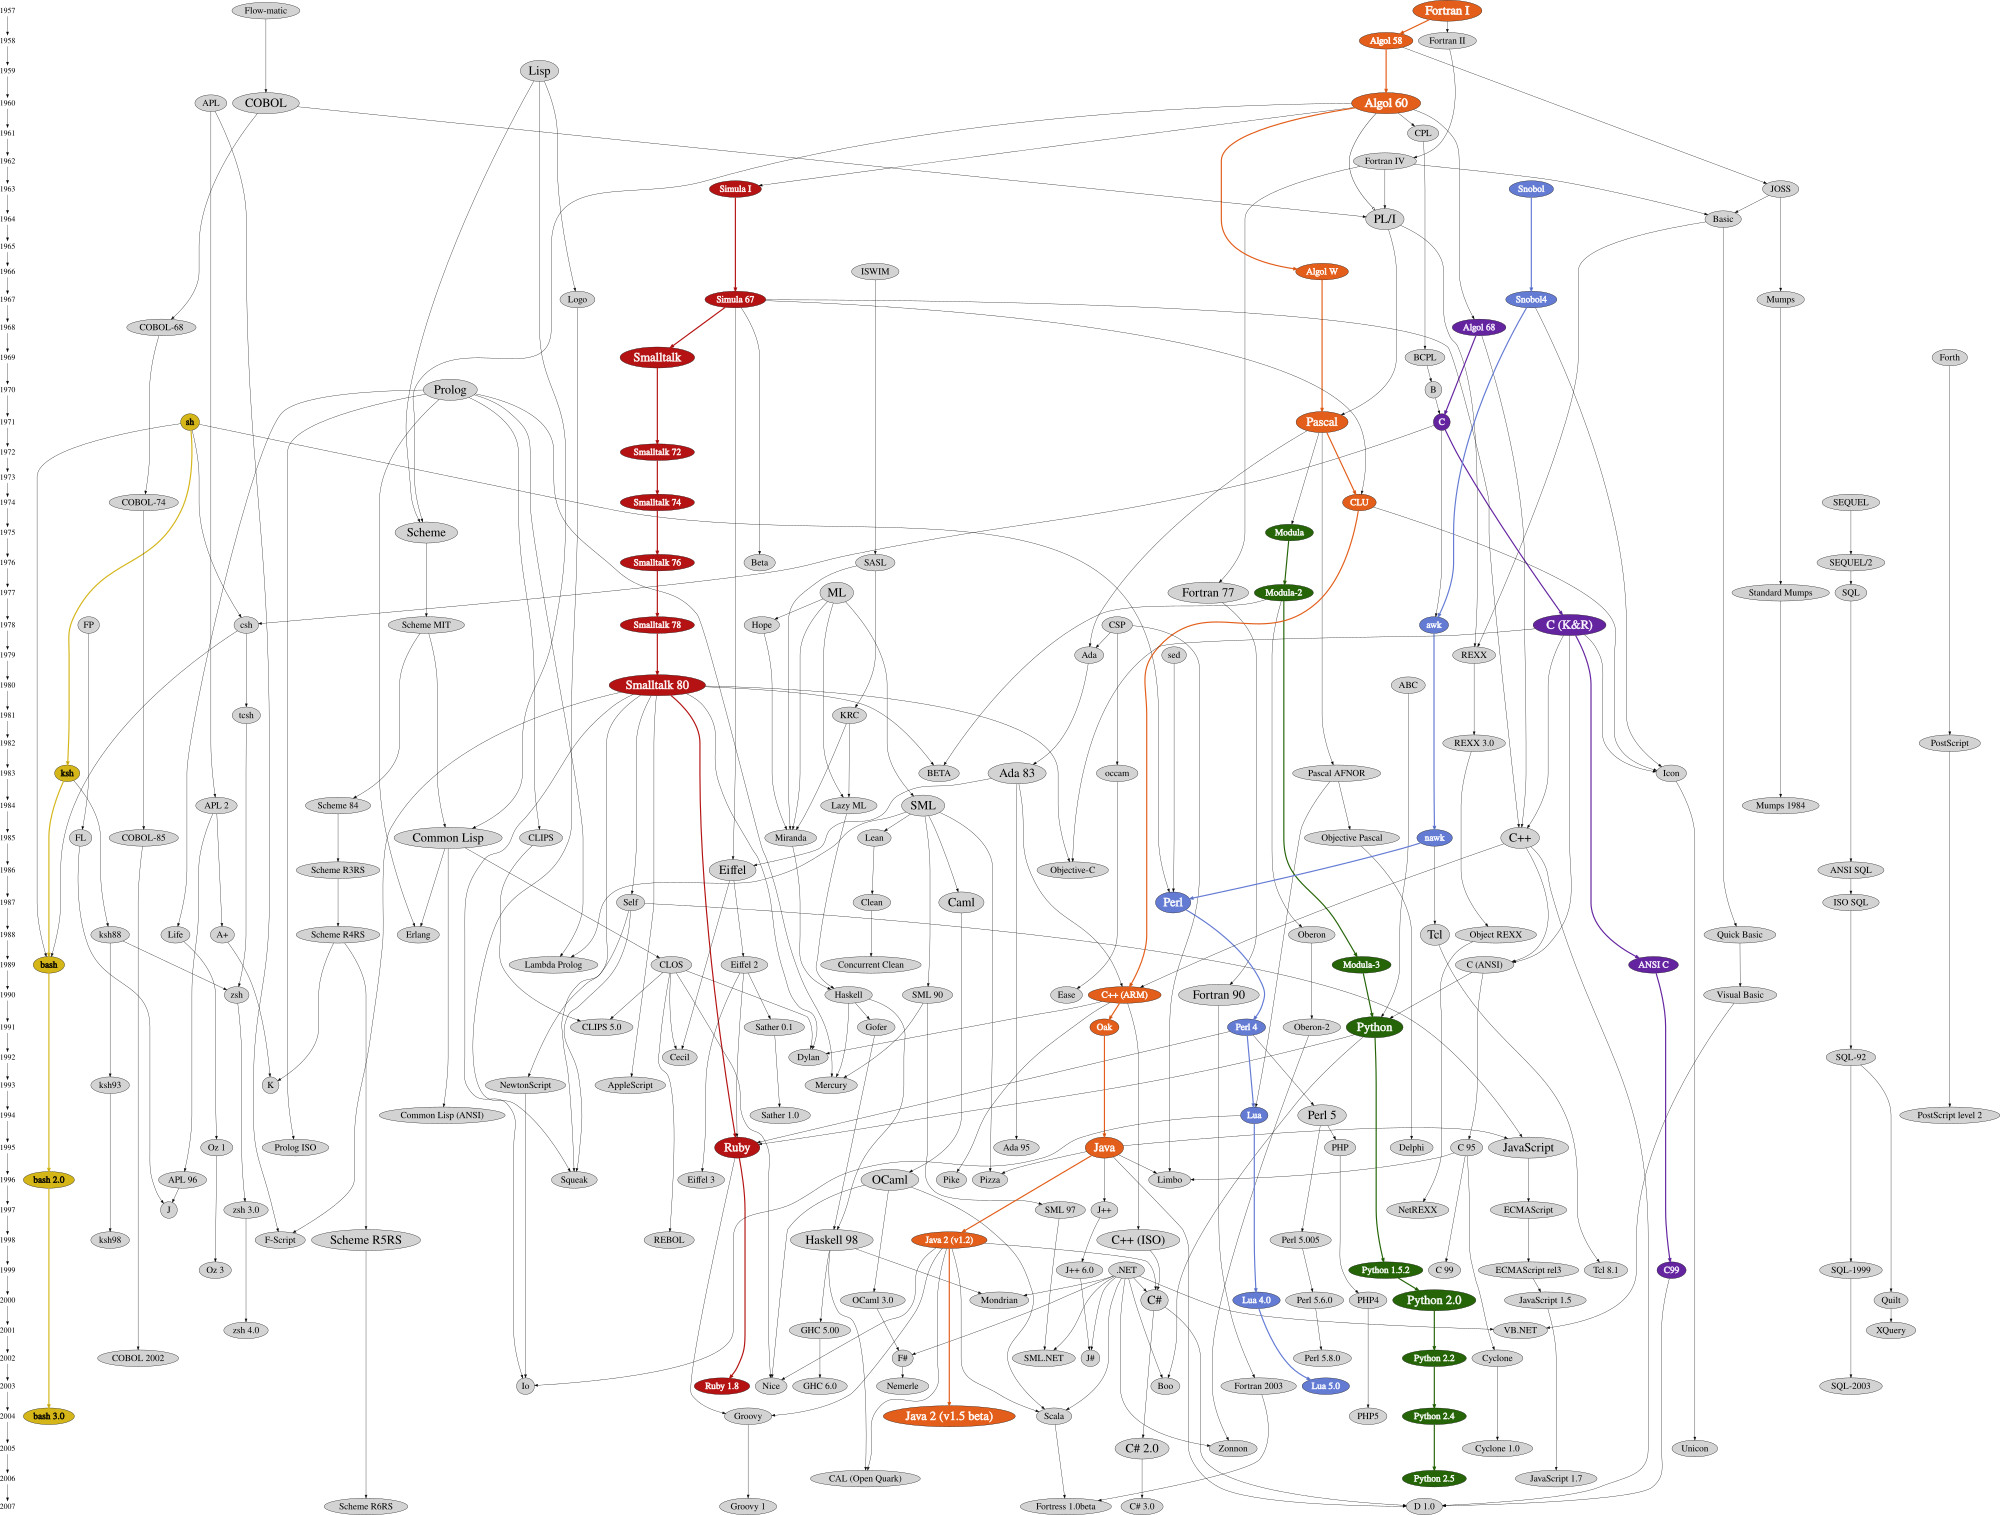
\includegraphics[width=.65\columnwidth]{../../../img/programming_language_tree.png}
\caption{Árvore Genealógica de \alert{Linguagens de Programação} (veja no \alert{site do curso})}
\end{figure}
\end{frame}

\section{Computação \& Ciência}
\label{sec:orga5a871c}
\begin{frame}[label={sec:orgaf6ce67}]{Tecnologia Computacional na Antiguidade: Melhores Usos\dots{}}
\begin{figure}[htbp]
\centering
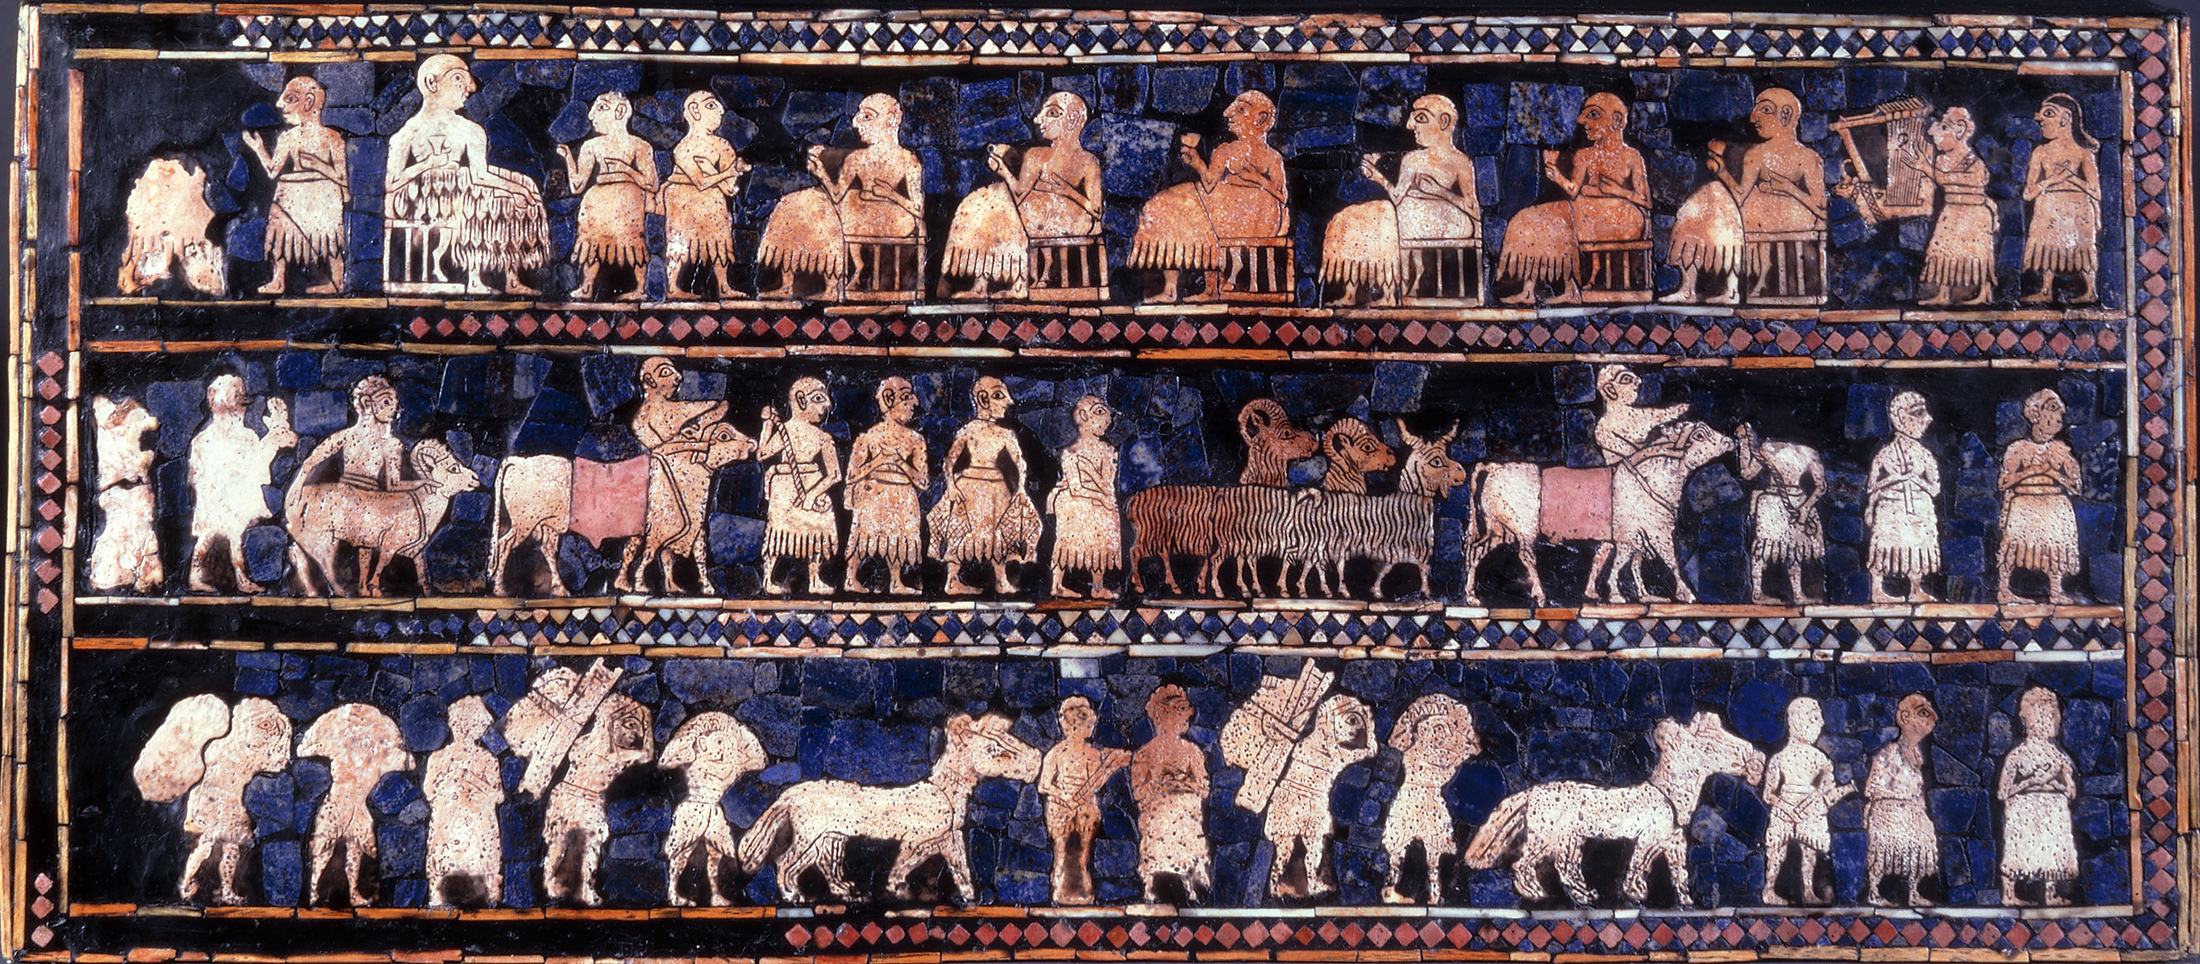
\includegraphics[width=\textwidth]{../../../img/ur_estandarte_paz.jpg}
\caption{Estandarte de Ur, \alert{lado paz}, 2600 AC}
\end{figure}
\end{frame}
\begin{frame}[label={sec:org39b04a1}]{Tecnologia Computacional na Antiguidade: \dots{}Piores Usos}
\begin{figure}[htbp]
\centering
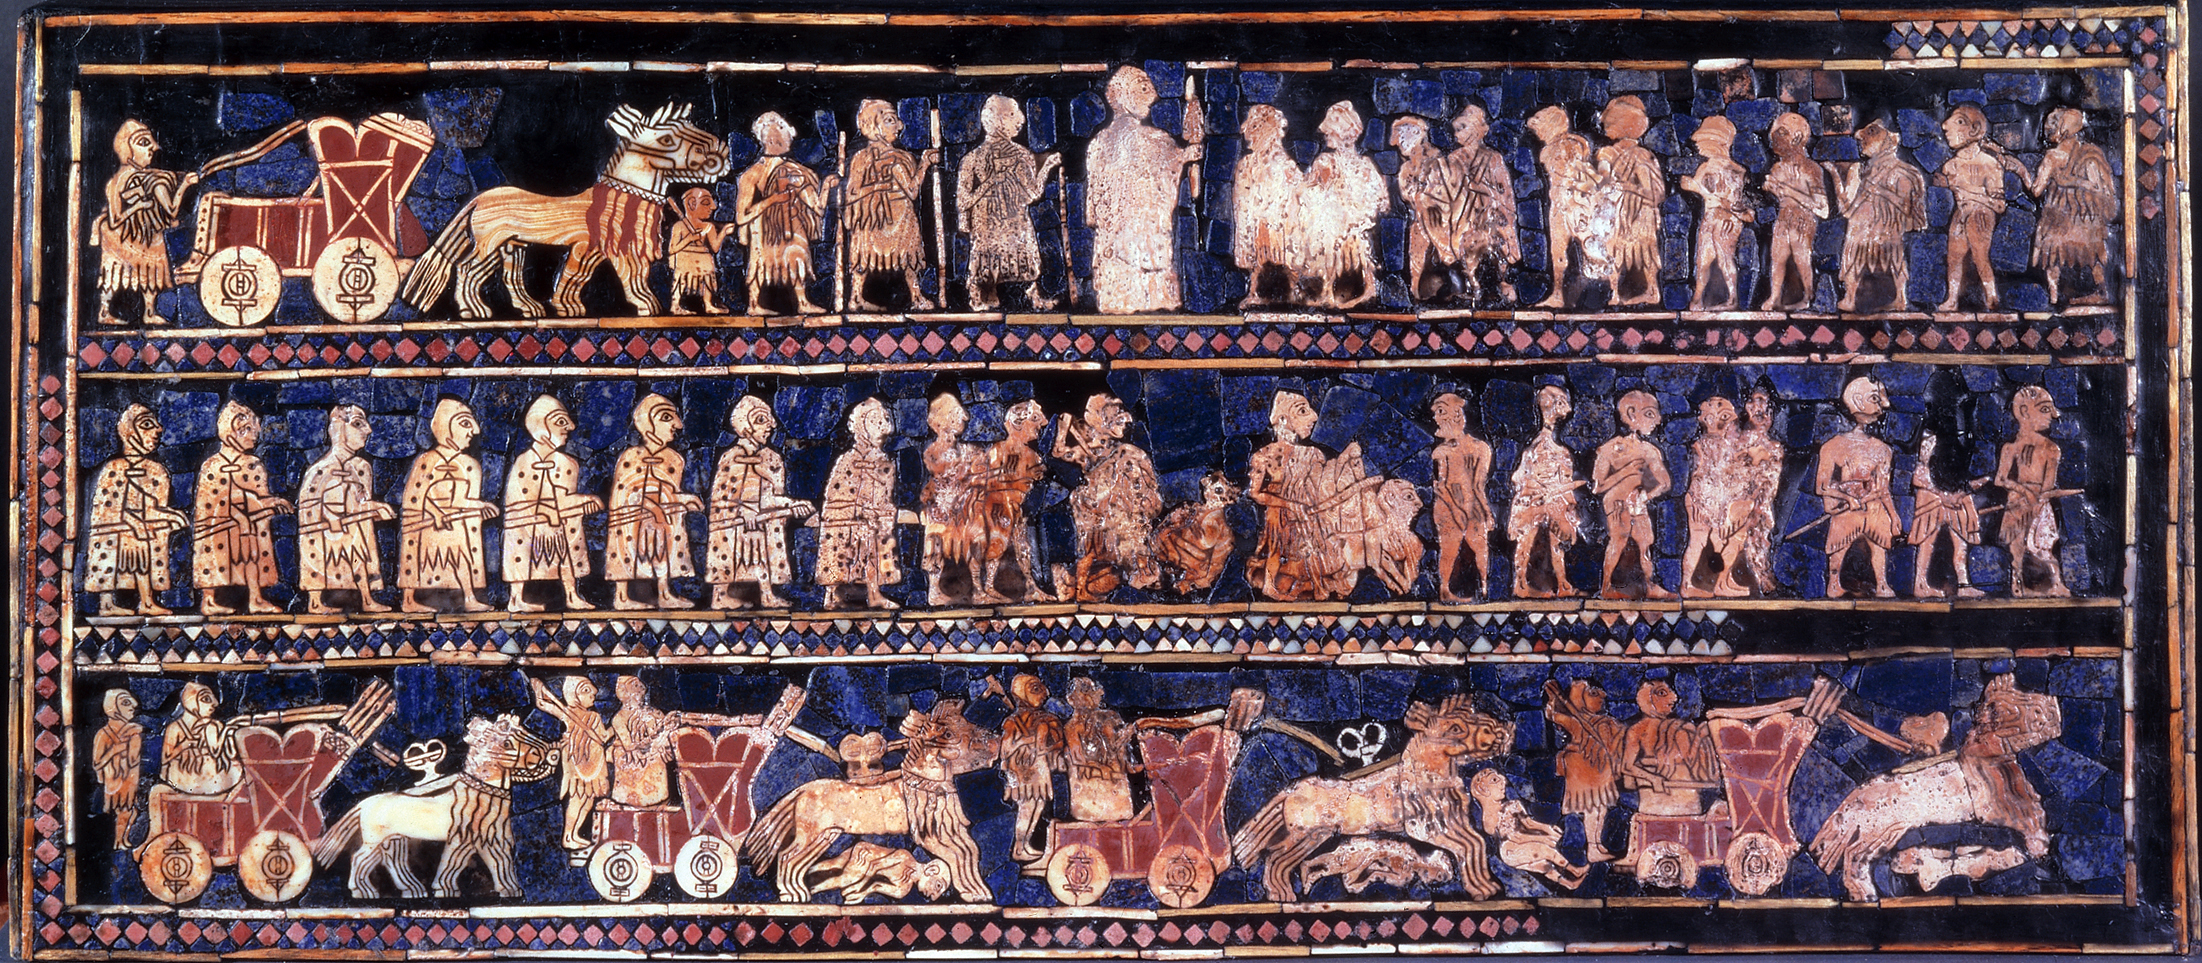
\includegraphics[width=\textwidth]{../../../img/ur_estandarte_guerra.jpg}
\caption{Estandarte de Ur, \alert{lado guerra}, 2600 AC}
\end{figure}
\end{frame}
\begin{frame}[label={sec:org56b1634},fragile]{Computação Hoje: Melhores Usos\dots{}}
 \begin{columns}
\begin{column}{0.5\columnwidth}
\begin{figure}[htbp]
\centering
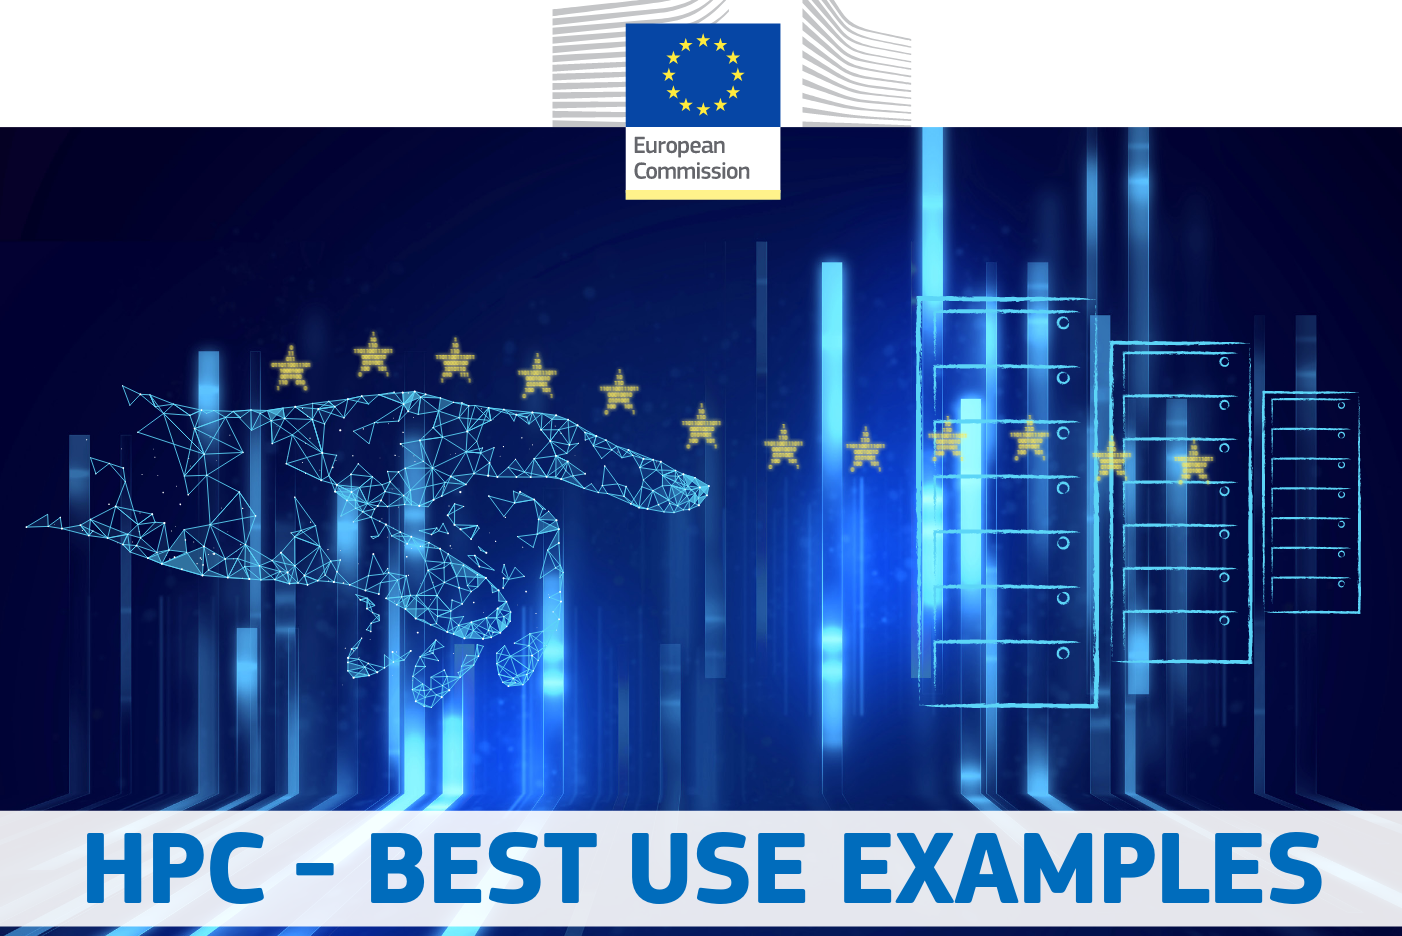
\includegraphics[width=\columnwidth]{../../../img/hpc_european_commission.png}
\caption{Relatório da \alert{Comissão Europeia} sobre os melhores usos da \alert{Computação de Alto-Desempenho}, 2018}
\end{figure}
\end{column}
\begin{column}{0.5\columnwidth}
\alert{Melhores} usos:
\begin{itemize}
\item Desenvolvimento de \alert{fármacos}
\item Mapeamento do \alert{cérebro humano}
\item Simulações \alert{climáticas} e \alert{sísmicas}
\item \alert{Planejamento urbano}
\item \alert{Astrofísica} e \alert{Cosmologia}
\end{itemize}

Você pode baixar o \texttt{pdf} aqui:
\begin{itemize}
\item \scriptsize\href{http://ec.europa.eu/newsroom/dae/document.cfm?doc_id=49301}{ec.europa.eu/newsroom/dae/document.cfm?doc\_id=49301}
\end{itemize}
\end{column}
\end{columns}
\end{frame}
\begin{frame}[label={sec:orge866d75}]{Computação Hoje: \dots{}Piores Usos}
\begin{columns}
\begin{column}{0.5\columnwidth}
\begin{figure}[htbp]
\centering
\includegraphics[height=.8\textheight]{../../../img/wmd_cover.jpg}
\caption{Capa do livro \alert{Armas de Destruição Matemática}, 2017}
\end{figure}
\end{column}
\begin{column}{0.5\columnwidth}
\alert{Piores} usos:
\begin{itemize}
\item \alert{Coleta ubíqua} de dados
\item Seu \alert{comportamento}:
\begin{itemize}
\item \alert{Análise} \(\rightarrow\) \alert{Predição} \(\rightarrow\) \alert{Geração}
\end{itemize}
\end{itemize}

Alguns \alert{livros interessantes}:
\begin{itemize}
\item \alert{The Age of Surveillance Capitalism}, 2018
\item \alert{Weapons of Math Destruction}, 2017
\item \alert{Data and Goliath}, 2015
\end{itemize}
\end{column}
\end{columns}
\end{frame}

\begin{frame}[label={sec:org3757282}]{Computação \& Ciência}
\begin{columns}
\begin{column}{0.5\columnwidth}
\begin{block}{\alert{Ubiquidade} da Computação na Ciência}
\begin{itemize}
\item Enorme \alert{volume de dados}
\item Modelos de \alert{análise} \& \alert{predição}
\item \alert{Comunicação} \& \alert{publicação}
\item Atividades do \alert{dia-a-dia}
\end{itemize}
\end{block}
\end{column}
\begin{column}{0.5\columnwidth}
\only<1>{
\begin{figure}[htbp]
\centering
\includegraphics[width=.8\columnwidth]{../../../img/lhc_mapa.png}
\caption{Mapa do \alert{Large Hadron Collider}}
\end{figure}
}

\only<2>{
\begin{figure}[htbp]
\centering
\includegraphics[width=\columnwidth]{../../../img/lhc_tunel.jpg}
\caption{Um corredor no \alert{Large Hadron Collider}}
\end{figure}
}
\end{column}
\end{columns}
\end{frame}
\begin{frame}[label={sec:orga105e76}]{Computação \& Ciência: Oceanografia}
\begin{columns}
\begin{column}{0.5\columnwidth}
\begin{block}{Computação \& Oceanografia}
\begin{itemize}
\item \href{http://www.cev.washington.edu/index.html}{Center for Environment Visualization}
\item \href{https://faculty.washington.edu/pmacc/LO/LiveOcean.html}{LiveOcean}: Simulações
\item \href{http://www.ncsa.illinois.edu/news/story/the\_fragile\_balance\_of\_the\_most\_productive\_ecosystems}{Simulando transporte de sedimentos}
\item \href{https://www.onepetro.org/conference-paper/ISOPE-I-02-281}{Modelagem de ondas e correntes}
\item \href{https://agupubs.onlinelibrary.wiley.com/doi/full/10.1002/2014GL062577}{Previsão de tsunamis}
\item \dots{}
\end{itemize}
\end{block}
\end{column}
\begin{column}{0.5\columnwidth}
\begin{figure}[htbp]
\centering
\includegraphics[width=\columnwidth]{../../../img/alpha_crucis.jpg}
\caption{\alert{Alpha Crucis}, o navio oceanográfico da USP}
\end{figure}
\end{column}
\end{columns}
\end{frame}
\begin{frame}[label={sec:org92feb23},fragile]{Computação \& Ciência: mini-EP1}
 \begin{block}{Computação \& Ciência: mini-EP1}
\begin{enumerate}
\item \alert{Encontre} um exemplo de \alert{pesquisa científica} que:
\begin{itemize}
\item Desperte o \alert{seu interesse}
\item Tenha sido \alert{facilitado} ou \alert{tornado possível} pela \alert{computação moderna}
\begin{itemize}
\item \alert{Sensores}, \alert{satélites}, \alert{volume de dados}, \alert{simulações}, \dots{}
\end{itemize}
\end{itemize}
\item \alert{Escreva um parágrafo} resumindo a pesquisa
\begin{itemize}
\item Inclua \alert{links} para a pesquisa
\end{itemize}
\item \alert{Entregue} um \alert{arquivo \texttt{pdf}} no \alert{PACA}
\begin{itemize}
\item Até a \alert{próxima Quinta, 08/08}
\end{itemize}
\end{enumerate}
\end{block}
\end{frame}
\maketitle
\end{document}
